% ------------------------------------------------------------------------
% ------------------------------------------------------------------------
% Monografia Peacon
% Trabalho de Conclusão de Curso
% Baseia-se no documento modelo de TCC do abntex2
% Para saber mais, acesse https://github.com/abntex/abntex2
% ------------------------------------------------------------------------
% ------------------------------------------------------------------------

\documentclass[
		% -- opções da classe memoir --
		12pt,				% tamanho da fonte
		openright,			% capítulos começam em pág ímpar (insere página vazia caso preciso)
		oneside,			% para impressão em verso e anverso. Oposto a oneside
		a4paper,			% tamanho do papel. 
		% -- opções da classe abntex2 --
		chapter=TITLE,		% títulos de capítulos convertidos em letras maiúsculas
		%section=TITLE,		% títulos de seções convertidos em letras maiúsculas
		%subsection=TITLE,	% títulos de subseções convertidos em letras maiúsculas
		%subsubsection=TITLE,% títulos de subsubseções convertidos em letras maiúsculas
		% -- opções do pacote babel --
		english,			% idioma adicional para hifenização
		brazil				% o último idioma é o principal do documento
	]{abntex2}


% ----------------------------------------------------------
% Pacotes básicos 
% ----------------------------------------------------------
%\usepackage{helvet}			
\usepackage[scaled]{helvet}
\renewcommand*\familydefault{\sfdefault} 	% Only if the base font of the document is to be sans serif
										% Foi necessário para acertar o documento, continha diversos erros
\usepackage[T1]{fontenc}		% Selecao de codigos de fonte.
\usepackage[utf8]{inputenc}	% Codificacao do documento (conversão automática dos acentos)
\usepackage{lastpage}		% Usado pela Ficha catalográfica
\usepackage{indentfirst}		% Indenta o primeiro parágrafo de cada seção.
\usepackage{color}			% Controle das cores
\usepackage{graphicx}		% Inclusão de gráficos
\usepackage{microtype} 		% para melhorias de justificação
% ----------------------------------------------------------
		

% ----------------------------------------------------------
% Pacotes adicionais, usados apenas no âmbito do Modelo Canônico do abnteX2
%% ----------------------------------------------------------
\usepackage{lipsum}				% para geração de dummy text
\usepackage{customizacoes} 		% customizações feitas pelo autor
% ----------------------------------------------------------


% ----------------------------------------------------------
% Pacotes de citações
% ----------------------------------------------------------
\usepackage[alf]{abntex2cite}				% Citações padrão ABNT

% ----------------------------------------------------------
% CONFIGURAÇÕES DE PACOTES
% ----------------------------------------------------------

% ----------------------------------------------------------
% Configurações do pacote backref
% ----------------------------------------------------------
\definecolor{thered}{rgb}{0.65,0.04,0.07}
\definecolor{thegreen}{rgb}{0.06,0.44,0.08}
\definecolor{thegrey}{gray}{0.5}
\definecolor{theshade}{rgb}{1,1,0.97}
\definecolor{theframe}{gray}{0.6}
% ----------------------------------------------------------


% ----------------------------------------------------------
% Informações de dados para CAPA e FOLHA DE ROSTO
% ----------------------------------------------------------

\titulo{Desenvolvimento de um Protótipo de Rastreador de Beacons utilizando o Raspberry Pi}
\autor{Gabriel Luiz Bastos Oliveira}
\local{Bauru}
\data{2015}
\orientador{Prof. Dr. Eduardo Martins Morgado}
\instituicao{%
  Universidade Estadual Paulista "Júlio de Mesquita Filho"
  \par
  Faculdade de Ciências - Campus Bauru
  \par
  Departamento de Computação
}
\tipotrabalho{Monografia (Trabalho de Conclusão de Curso)}
% O preambulo deve conter o tipo do trabalho, o objetivo, 
% o nome da instituição e a área de concentração 
% foi necessário utilizar \~{a} e etc para os acentos por problemas na geração do PDF
\preambulo{Trabalho de Conclus\~{a}o de Curso apresentado ao Departamento de Computa\c{c}\~{a}o da Faculdade de Ci\^{e}ncias da Universidade Estadual Paulista “J\'{ú}lio de Mesquita Filho” – UNESP, C\^{a}mpus de Bauru.}

% ----------------------------------------------------------


% ----------------------------------------------------------
% Configurações de aparência do PDF final
% ----------------------------------------------------------

% alterando o aspecto da cor azul
\definecolor{blue}{RGB}{0,0,0}

% informações do PDF
\makeatletter
\hypersetup{
     	%pagebackref=true,
		pdftitle={\@title}, 
		pdfauthor={\@author},
    	pdfsubject={\imprimirpreambulo},
	    pdfcreator={LaTeX with abnTeX2},
		pdfkeywords={beacon}{raspberry pi}{internet das coisas}{abntex2}{trabalho acadêmico}, 
		colorlinks=true,       		% false: boxed links; true: colored links
    	linkcolor=blue,          	% color of internal links
    	citecolor=blue,        		% color of links to bibliography
    	filecolor=magenta,      		% color of file links
		urlcolor=blue,
		bookmarksdepth=4
}
\makeatother
% ----------------------------------------------------------


% ----------------------------------------------------------
% Espaçamentos entre linhas e parágrafos 
% ----------------------------------------------------------

% O tamanho do parágrafo é dado por:
\setlength{\parindent}{1.3cm}

% Controle do espaçamento entre um parágrafo e outro:
\setlength{\parskip}{0.2cm}  % tente também \onelineskip

% ----------------------------------------------------------
% compila o indice
% ----------------------------------------------------------
\makeindex
% ----------------------------------------------------------


% ----------------------------------------------------------
% Configurações de projeto
% ----------------------------------------------------------
\newif\iffinal
\finaltrue % define se é um arquivo final, se for não for retira umas partes. 

\newif\ifrelatorio
\relatoriofalse % define se é um arquivo final, se for não for retira umas partes. 

\newif\ifabstract
\abstractfalse % define se mostra o abstract em inglês ou não.

\newif\ifresumo
\resumotrue % define se mostra o resumo ou não.

\newif\ifficha
\fichafalse % define se mostra a ficha catalográfica ou não
% ----------------------------------------------------------


% ----------------------------------------------------------
% Início do documento
% ----------------------------------------------------------
\begin{document}

% Seleciona o idioma do documento (conforme pacotes do babel)
%\selectlanguage{english}
\selectlanguage{brazil}

% Retira espaço extra obsoleto entre as frases.
\frenchspacing 

% ----------------------------------------------------------
% ELEMENTOS PRÉ-TEXTUAIS
% ----------------------------------------------------------
\pretextual


% ----------------------------------------------------------
% Capa
% ----------------------------------------------------------
\imprimircapa
% ----------------------------------------------------------


% ----------------------------------------------------------
% Folha de rosto
% (o * indica que haverá a ficha bibliográfica)
% ----------------------------------------------------------
\imprimirfolhaderosto
% ----------------------------------------------------------


% ----------------------------------------------------------
% Inserir a ficha catalográfica
% ----------------------------------------------------------

% Isto é um exemplo de Ficha Catalográfica, ou "Dados internacionais de
% catalogação-na-publicação''. Você pode utilizar este modelo como referência. 
% Porém, provavelmente a biblioteca da sua universidade lhe fornecerá um PDF
% com a ficha catalográfica definitiva após a defesa do trabalho. Quando estiver
% com o documento, salve-o como PDF no diretório do seu projeto e substitua todo
% o conteúdo de implementação deste arquivo pelo comando abaixo:
%
% \begin{fichacatalografica}
%     \includepdf{fig_ficha_catalografica.pdf}
% \end{fichacatalografica}

\ifficha
  \begin{fichacatalografica}
	\sffamily
	\vspace*{\fill}					% Posição vertical
	\begin{center}					% Minipage Centralizado
	\fbox{\begin{minipage}[c][8cm]{13.5cm}		% Largura
	\small
	\imprimirautor
	%Sobrenome, Nome do autor
	
	\hspace{0.5cm} \imprimirtitulo  / \imprimirautor. --
	\imprimirlocal, \imprimirdata-
	
	\hspace{0.5cm} \pageref{LastPage} p. : il. (algumas color.) ; 30 cm.\\
	
	\hspace{0.5cm} \imprimirorientadorRotulo~\imprimirorientador\\
	
	\hspace{0.5cm}
	\parbox[t]{\textwidth}{\imprimirtipotrabalho~--~\\ \imprimirinstituicao,
	\imprimirdata.}\\
	
	\hspace{0.5cm}
		1. Beacon.
		2. Raspberry Pi.
		3. Internet das Coisas.
		I. \imprimirorientador.
		II. Universidade Estadual Paulista "Júlio de Mesquita Filho".
		III. Faculdade de Ciências.
		IV. Título
	\end{minipage}}
	\end{center}
  \end{fichacatalografica}
\fi
% ----------------------------------------------------------


% ----------------------------------------------------------
% Inserir errata
% ----------------------------------------------------------
%\begin{errata}
%Elemento opcional da \citeonline[4.2.1.2]{NBR14724:2011}. Exemplo:

%\vspace{\onelineskip}

%FERRIGNO, C. R. A. \textbf{Tratamento de neoplasias ósseas apendiculares com
%reimplantação de enxerto ósseo autólogo autoclavado associado ao plasma
%rico em plaquetas}: estudo crítico na cirurgia de preservação de membro em
%cães. 2011. 128 f. Tese (Livre-Docência) - Faculdade de Medicina Veterinária e
%Zootecnia, Universidade de São Paulo, São Paulo, 2011.

%\begin{table}[htb]
%\center
%\footnotesize
%\begin{tabular}{|p{1.4cm}|p{1cm}|p{3cm}|p{3cm}|}
%  \hline
%   \textbf{Folha} & \textbf{Linha}  & \textbf{Onde se lê}  & \textbf{Leia-se}  \\
%    \hline
%    1 & 10 & auto-conclavo & autoconclavo\\
%   \hline
%\end{tabular}
%\end{table}

%\end{errata}
% ----------------------------------------------------------


% ----------------------------------------------------------
% Inserir folha de aprovação
% ----------------------------------------------------------

% Isto é um exemplo de Folha de aprovação, elemento obrigatório da NBR
% 14724/2011 (seção 4.2.1.3). Você pode utilizar este modelo até a aprovação
% do trabalho. Após isso, substitua todo o conteúdo deste arquivo por uma
% imagem da página assinada pela banca com o comando abaixo:
%
% \includepdf{folhadeaprovacao_final.pdf}
%
\begin{folhadeaprovacao}
	\begin{center}
		{\ImprimirAutor}
		
		\vspace*{\fill}\vspace*{\fill}
		\begin{center}
			\bfseries\large\ImprimirTitulo
		\end{center}
		\vspace*{\fill}
   
		\hspace{.45\textwidth}
		\begin{minipage}{.5\textwidth}
			\imprimirpreambulo
		\end{minipage}%
		\vspace*{\fill}
     
		%Trabalho aprovado. \imprimirlocal, 24 de novembro de 2012:
   
		\uppercase{Banca examinadora}
	\end{center}
	
	Aprovado em \detokenize{___/___/___}.

	\assinatura{\textbf{\imprimirorientador} \\ Orientador} 
	\assinatura{\textbf{Prof. Dr. Aparecido Nilceu Marana}}
	\assinatura{\textbf{Profa. Dra. Márcia A. Z. Meira e Silva}}
	%\assinatura{\textbf{Professor} \\ Convidado 3}
	%\assinatura{\textbf{Professor} \\ Convidado 4}
	
	\vspace*{0.5cm}
	\hspace{.5\textwidth}
	\begin{center} 
		{ \ImprimirLocal \\ \imprimirdata }
	\end{center}
\end{folhadeaprovacao}
% ----------------------------------------------------------


% ----------------------------------------------------------
% Dedicatória
% ----------------------------------------------------------
\ifrelatorio
	\begin{dedicatoria} 
		\vspace*{\fill}
		\centering
		\noindent
		\textit{ Este trabalho é dedicado às crianças adultas que,\\
				quando pequenas, sonharam em se tornar cientistas.} 
		\vspace*{\fill}
	\end{dedicatoria}
\fi
% ----------------------------------------------------------


% ----------------------------------------------------------
% Agradecimentos
% ----------------------------------------------------------
\iffinal
	\begin{agradecimentos}

Agradeço ao meu orientador Prof. Dr. Eduardo Morgado, por todo o tempo e trajetória no LTIA\footnote{Laboratório de Tecnologia da Informação Aplicada}, pela confiança, apoio e incentivo. Agradeço também pelo auxílio em todas as etapas desse projeto, desde a definição do tema até a apresentação final.

A Henrique Lopes Santos, pela ajuda na realização das fotos e também criação do logotipo para o protótipo.

A Elisa Castro, pelo apoio na correção e melhorias na digitação do texto contido nesse documento.

A Giovanna Aguirre, pelo apoio, incentivo, paciência e companhia nos momentos mais importantes de minha vida.

A todos os colegas do laboratório, pela incrível parceria, trabalho em equipe e organização de projetos. Os quatro anos percorridos com eles foram essenciais para meu crescimento profissional e pessoal.

A todos os professores, pois com muito esforço diário passaram não somente as informações técnicas e práticas de cada disciplina, mas lições que servirão para toda vida.

A todos os colegas de curso, que de alguma forma auxiliaram a chegar ao último semestre da melhor maneira possível.

Aos meus amigos e familiares, pelo apoio e incentivo na escolha e decorrer do curso, com muita compreensão e encorajamento.

	\end{agradecimentos}
\fi
% ----------------------------------------------------------


% ----------------------------------------------------------
% Epígrafe
% ----------------------------------------------------------
\iffinal
	\begin{epigrafe}
		\vspace*{\fill}
			\begin{flushright}
			%\textit{"Sonhos não morrem, apenas \\ 
			%	 adormecem na alma da gente."\\
			%(Francisco Cândido Xavier)}
			\textit{"Que eu não perca a vontade de ajudar as pessoas, \\
				mesmo sabendo que muitas delas são incapazes \\
				de ver, reconhecer e retribuir esta ajuda."\\
				(Francisco Cândido Xavier)}
		\end{flushright}
	\end{epigrafe}
\fi
% ----------------------------------------------------------


% ----------------------------------------------------------
% RESUMOS
% ----------------------------------------------------------
\ifresumo
	% resumo em português
	\setlength{\absparsep}{18pt} % ajusta o espaçamento dos parágrafos do resumo
	\begin{resumo}

	 		FALTA ACERTAR!!!!!! Atualmente a área da internet das coisas tem recebido um foco enorme. Um dos motivos é devido a ser bem nova e também facilitar a integração das pessoas com o mundo real. Essa área tem motivado várias pessoas pela possibilidade de ter um produto concreto após pouco tempo de trabalho. Por conta disso, alguns dispositivos foram criados para auxiliar essas áreas, entre eles o \textit{Arduino} e \textit{Raspberry Pi}. Os \textit{beacons} também são uma criação nova, comunicando com outros dispositivos maiores como o \textit{RPi} para auxiliar a micro-localização dentro de um pequeno espaço, com um baixo custo. O seu foco de uso é pequeno, somente com leituras via \textit{smartphones}. Esse projeto tem como objetivo criar um rastreador de \textit{beacons} utilizando o \textit{Raspberry Pi} para expandir essa capacidade, não necessitando de um celular para que os \textit{beacons} possam ser encontrados.

 			\textbf{Palavras-chave}: \textit{Beacon}. Raspberry Pi. Internet das Coisas.
 			
	\end{resumo}
	
	% resumo em inglês
	\begin{resumo}[Abstract]
	 	\begin{otherlanguage*}{english}
			This is the english abstract.

			\textbf{Keywords}: Beacon. Raspberry Pi. Internet of Things.
		\end{otherlanguage*}
	\end{resumo}
	
\fi
% ----------------------------------------------------------


% ----------------------------------------------------------
% inserir lista de ilustrações
% ----------------------------------------------------------
\iffinal
	\pdfbookmark[0]{\listfigurename}{lof}
	\listoffigures*
	\cleardoublepage
\fi
% ----------------------------------------------------------


% ----------------------------------------------------------
% inserir lista de tabelas
% ----------------------------------------------------------
\iffinal
	\pdfbookmark[0]{\listtablename}{lot}
	\listoftables*
	\cleardoublepage
\fi
% ----------------------------------------------------------


% ----------------------------------------------------------
% inserir lista de abreviaturas e siglas
% ----------------------------------------------------------
\iffinal
	\begin{siglas}
			\item[IoT] \textit{Internet of Things} - Internet das Coisas
			\item[DIY] \textit{Do It Yourself} - Faça Você Mesmo
			\item[RPi] \textit{Raspberry Pi}
			\item[GPIO] \textit{General Input and Output}
			\item[BLE] \textit{Bluetooth Low Energy}
			\item[LTIA] Laboratório de Tecnologia da Informação Aplicada
	\end{siglas}
\fi
% ----------------------------------------------------------


% ----------------------------------------------------------
% inserir lista de símbolos
% ----------------------------------------------------------
%\iffinal
%	\begin{simbolos}
%			\item[$ \Gamma $] Letra grega Gama
%			\item[$ \Lambda $] Lambda
%			\item[$ \zeta $] Letra grega minúscula zeta
%			\item[$ \in $] Pertence
%	\end{simbolos}
%\fi
% ----------------------------------------------------------


% ----------------------------------------------------------
% inserir o sumario
% ----------------------------------------------------------
\pdfbookmark[0]{\contentsname}{toc}
\tableofcontents*
\cleardoublepage
% ----------------------------------------------------------



% ----------------------------------------------------------------------------------------------------------------------------------



% ----------------------------------------------------------------------------------------------------------------------------------
% ELEMENTOS TEXTUAIS
% ----------------------------------------------------------------------------------------------------------------------------------
\textual


% ----------------------------------------------------------
% Introdução
% ----------------------------------------------------------

% ----------------------------------------------------------
% Introdução
% ----------------------------------------------------------
\chapter{Introdução}\label{cap:introducao}
%\addcontentsline{toc}{chapter}{Introdução}
% ----------------------------------------------------------

A internet cresce dia após dia e cada vez mais diferentes tipos de dispositivos são conectados a essa imensa rede. Há uma estimativa de 26 bilhões de ''coisas'' conectadas a internet até 2020, comparado a 6 bilhões na década de 2000. Isso foi possível graças ao custo do acesso a internet e banda larga terem diminuído 40 vezes nos últimos 10 anos. Esse \textit{boom} de crescimento também é influenciado pela IoT (\textit{Internet of Things} - Internet das Coisas). \cite{goldmansachs-iot}. 

Segundo \citeonline{ashton-iot} o termo IoT surgiu como título de sua apresentação à Procter \& Gamble (P\&G) em 1999. Esse termo advém do uso de internet em diferentes tipos de dispositivos. 

\begin{citacao}
''(...) a Internet das Coisas é um conceito no qual dispositivos de nosso dia a dia são equipados com sensores capazes de captar aspectos do mundo real, como por exemplo, temperatura, umidade, presença, etc, e envia-los a centrais que recebem estas informações e as utilizam de forma inteligente.'' \cite{nascimento-iot}.
\end{citacao}

Como exemplo podemos citar: geladeira ligada a internet informando a falta de condimentos, caixa de remédio conectada a internet prevendo o término de remédio para avisar ao consumidor, entre diversos outros. Um bom exemplo é interligar uma casa por meio de sensores, como termostatos, sistemas de segurança, iluminação, sistemas de entretenimento com uma inteligência por trás para diversas aplicações. \cite{goldmansachs-iot}

Diversas áreas tiveram o seu crescimento alavancado por conta da IoT. O mais marcante é o ramo do DIY (\textit{Do It Yourself}, ou faça você mesmo), em que pessoas criam ou adaptam coisas para suas necessidades. Isso se dá por conta de ter aparecido no mercado dispositivos e componentes que auxiliam a criação e adaptação de eletrônicos e outros. Um ótimo exemplo é o Arduino, um dispositivo que ajuda a criar os projetos de eletrônica e que é composto de duas partes: o hardware e o software. Com eles é possível construir praticamente de tudo, desde um LED piscante a um robô que envia um \textit{tweet} quando sua planta está sem água. \cite{ben-arduino}. \cite{sorrel-arduino}.

Além do Arduino existem diversos outros \textit{devices} com funcionalidades similares ou até complementares. Podemos citar o \textit{Raspberry Pi}, um computador do tamanho de um cartão de crédito e de baixo custo. \cite{raspberrypi-rpi}. Por ser um computador é possível executar um sistema operacional (como Linux, \textit{RISC OS}, \textit{Windows 10 for IoT}). Dependendo do modelo possui portas USB (1 a 4) para conexão com periféricos (como mouse, teclado, adaptador WiFi, Bluetooth), e também porta Ethernet para conexão a internet cabeada (exceto modelo A e A+). Também possui de 26 (modelo A e B) a 40 pinos (modelo A+, B+ e 2) para conexões gerais de entrada e saída digitais (GPIO - \textit{General Input and Output}). 

Através desses pinos pode-se conectar uma diversidade de componentes eletrônicos como sensores, atuadores, outros dispositivos para comunicação. Dessa forma, suas funcionalidades são expandidas de uma forma absurda, ficando a cargo de cada pessoa montar uma nova aplicação. Uma boa aplicação é a conexão de um adaptador bluetooth pela USB para comunicação com smartphones, tablets, PCs e outros dispositivos tipo sensores sem fio.

Um exemplo desses sensores externos são os \textit{beacons}, pequenos modelos sem fio que se comunicam por meio do Bluetooth 4.0 ou BLE (\textit{Bluetooth Low Energy} - Bluetooth de Baixa Energia). Como o próprio nome diz, esse padrão de comunicação utiliza pouca energia. Desta forma, um \textit{beacon} pode funcionar por anos. ''Na prática, ela permite localizar objetos (ou pessoas que carregam esses objetos) com muito mais precisão dentro de ambientes fechados.'' \cite{teixeira-beacon}.

Os \textit{beacons} foram pouco explorados até o momento, seu uso está sendo mais notado na área de grandes lojas do varejo.

\begin{citacao}
''A Apple (...) já está utilizando a tecnologia em 254 lojas nos EUA. As funcionalidades já estão embutidas na versão oficial do aplicativo da Apple Store para iOS [, sistema operacional de seus smartphones e tablets]. (...) Quando o usuário se aproxima de uma loja física, o aplicativo oferece toda uma camada extra de informações e serviços que são específicos para aquela unidade – como por exemplo ofertas locais, tamanho da fila para ser atendido no Genius Bar, eventos e treinamentos que estão agendados ali na loja etc.'' \cite{teixeira-beacon}.
\end{citacao}

A Macy's (grande rede norte americana de loja de departamentos) realizou testes em algumas de suas lojas para enviar alertas a pessoas que entrarem em suas lojas, com promoções e melhores indicações, utilizando o padrão \textit{iBeacon} da Apple. Os testes foram limitados a usuários de iPhone, e somente quando entraram na loja. Em um futuro teste espera-se que seja possível separar por departamentos, para que quando um usuário percorra a loja apareça as notícias relativas ao local da loja que ela está. \cite{kastrenakes-macys-beacon}


% ---
% Objetivos
% ---
\section{Objetivos}\label{cap:objetivos-justificativa}
% ---

% ---
% Objetivos Gerais
% ---
\subsection{Objetivos Gerais}\label{sec:objetivos-gerais}
% ---

O objetivo geral desse projeto é projetar e desenvolver um dispositivo rastreador de \textit{iBeacons} utilizando o \textit{Raspberry Pi}.

% ---

% ---
\subsection{Objetivos Específicos}\label{sec:objetivos-especificos}
% ---

\begin{alineas}
	\item Estudar o funcionamento de \textit{beacons}, comunicação via \textit{bluetooth low energy} e \textit{Raspberry Pi}, assim como suas aplicações;
	\item Identificar os requerimentos básicos de funcionamento de \textit{beacons} e \textit{Raspberry Pi};
	\item Definir os elementos para desenvolvimento do protótipo;
	\item Planejar a estrutura do sistema;
	\item Implementar o protótipo de acordo com a estrutura e elementos planejados.
\end{alineas}

% ---


% ---
\section{Logotipo e Nome para o Dispositivo}\label{sec:logotipo-prototipo}
% ---

Por ser um produto, decidiu-se que o dispositivo deveria ter um nome e logotipo. Durante algumas reuniões de \textit{brainstorm}, o nome \textit{Peacon} surgiu e foi o escolhido. Esse nome deriva das palavras \textit{Pi}  + \textit{beacon}. Nos próximos capítulos o dispositivo rastreador será referido conforme seu nome.

Juntando todos os atributos do Peacon, criou-se um logotipo\footnote{O logotipo foi criado por Henrique Lopes Silva Santos, aluno do curso de Design da Faculdade de Arquitetura, Artes e Comunicação da UNESP de Bauru.} que identificasse muito bem todas as suas funcionalidades (\autoref{fig:logo-peacon}). Adesivos foram criados para colar no protótipo e identificar o produto.

\begin{figure}[htb]
	\caption{\label{fig:logo-peacon}Logotipo criado para o protótipo}
	\begin{center}
		
\includegraphics[width=0.5\textwidth]{img/logo-peacon.png}
	\end{center}
	\legend{Fonte: elaborado pelo autor}
\end{figure}

% ----------------------------------------------------------

% ----------------------------------------------------------


% ----------------------------------------------------------
% Objetivos
% ----------------------------------------------------------

% ----------------------------------------------------------
% Objetivos
% ----------------------------------------------------------
\chapter{Objetivos}\label{cap:objetivos-justificativa}
% ----------------------------------------------------------

% ---
% Objetivos Gerais
% ---
\section{Objetivos Gerais}\label{sec:objetivos-gerais}
% ---

O objetivo geral desse projeto é planejar e desenvolver um protótipo de rastreador de \textit{iBeacons} utilizando o \textit{Raspberry Pi}.

% ---

% ---
\section{Objetivos Específicos}\label{sec:objetivos-especificos}
% ---

\begin{alineas}
	\item Estudar o funcionamento de \textit{beacons}, comunicação via \textit{bluetooth low energy} e \textit{Raspberry Pi}, assim como suas aplicações.
	\item Identificar os requerimentos básicos de funcionamento de \textit{beacons} e \textit{Raspberry Pi}.
	\item Definir os elementos para desenvolvimento do protótipo.
	\item Planejar a estrutura do sistema.
	\item Implementar o protótipo de acordo com a estrutura e elementos planejados.
\end{alineas}

% ----------------------------------------------------------

% ----------------------------------------------------------


% ----------------------------------------------------------
% Fundamentação Teórica
% ----------------------------------------------------------

% ----------------------------------------------------------
% Fundamentação Teórica
% ----------------------------------------------------------
\chapter{Fundamentação Teórica}\label{cap:fundamentacao-teorica}
% ----------------------------------------------------------

% ---
\section{Internet das Coisas}\label{sec:internet-das-coisas}
% ---

A área de IoT está em uma onda crescente, com um grande número de pessoas investindo nesse mercado, e um bom número de profissionais migrando para essa área. Há uma estimativa de que existem 19 milhões de profissionais trabalhando na indústria de desenvolvimento de software, e desses, 19\% trabalham em algum projeto relacionado a IoT. \cite{cw-iot}.

\begin{citacao}
''A próxima onda na era da computação será fora do domínio do ambiente de trabalho tradicional. No paradigma da IoT, muitos dos objetos que nos rodeiam estarão na rede de uma forma ou de outra. RFID (Radio Frequency Identification - Identificadores via Rádio Frequência) e as tecnologias de redes de sensores crescerão para enfrentar este novo desafio, em que os sistemas de informação e comunicação estão embutidos nos ambientes que nos rodeiam, de forma invisível.''. \cite{iot-article}. 
\end{citacao}

É notável o crescimento dessa área. Há uma expectativa de que, em 2020, o número de carros conectados a internet supere o número de carros não conectados, sendo esses carros possíveis de se comunicar com outros veículos e a infraestrutura das ruas, como os semáforos. \cite{goldmansachs-iot}. Segundo \citeonline{press-iot}, em 2014 a IoT substituiu a área da \textit{Big Data} como a tecnologia mais empolgante, ou seja, a tecnologia que mais pessoas iriam migrar e se interessar. 


% ---
\section{Raspberry Pi}\label{sec:raspberry-pi}
% ---

Quando se pesquisa algo sobre IoT é praticamente impossível não achar relação e links para \textit{Raspberry Pi}, Arduinos, e toda a área de \textit{DIY}. Atualmente existem três modelos, conforme a \autoref{table:comparativo-rpi} e \autoref{fig:todos-rpi}. 

\begin{figure}[htb]
	\caption{\label{fig:todos-rpi}\textit{RPi} A+ (esquerda), B+ (centro) e 2 Modelo B (direita).}
	\begin{center}
		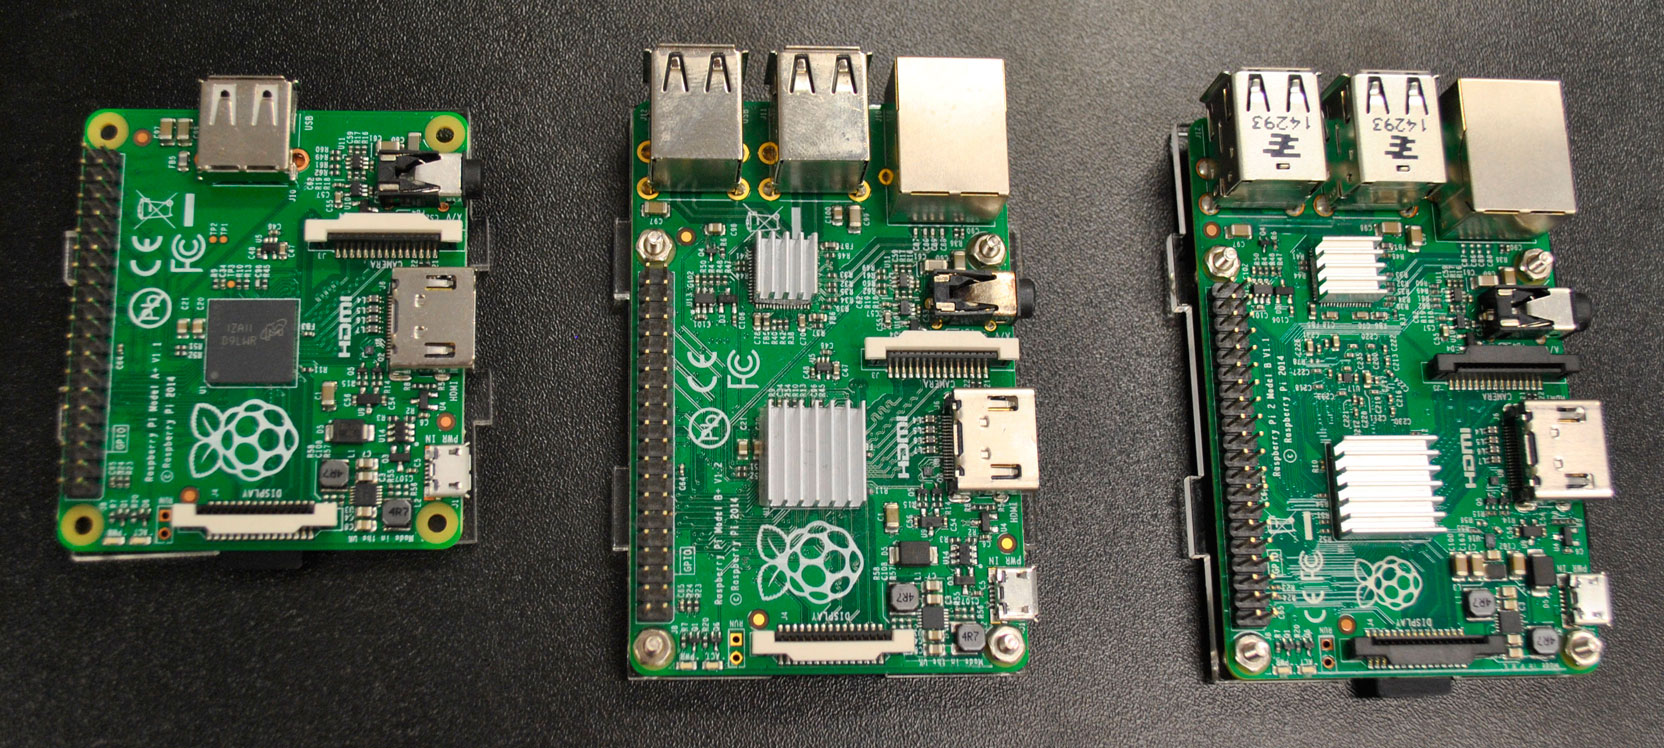
\includegraphics[width=0.8\textwidth]{img/rpi-modelos.jpg}
	\end{center}
	\legend{Fonte: elaborado pelo autor}
\end{figure}

\begin{table}[htb]
	\IBGEtab{%
  		\caption{Comparativo entre os modelos de \textit{Raspberry Pi}}%
  		\label{table:comparativo-rpi}
	}{%
  		\begin{tabular}{cccc}
	  		\toprule
	 			Versão & A+ & B+ & 2 Modelo B \\
  			\midrule \midrule
				Processador & ARMv6 single core & ARMv6 single core & ARMv7 quad core \\
			\midrule
				Velocidade CPU & 700 MHz single-core & 700 MHz single-core & 900 MHz quad-core \\
			\midrule 
				Memória RAM & 256 MB & 512 MB & 1 GB \\
  			\midrule 
				Portas USB & 1  & 4  & 4 \\
			\midrule 
				\textit{Ethernet} & Não & Sim  & Sim \\
  			\bottomrule
		\end{tabular}%
	}{%
  		\fonte{\cite{rpiversion-table}}%
  	}
\end{table}

Segundo \citeonline{raspberrypi-rpi}, esse pequeno dispositivo foi criado com intuito de ser utilizado por crianças e pessoas carentes do mundo todo para aprender programação e computação. É facilmente configurável, utilizando um cartão de memória como HD para o sistema operacional e dados.

Por meio de suas portas de entrada e saída digitais é possível conectar uma gama ampla de sensores, atuadores, componentes eletrônicos, ficando a cargo do programador e criador do projeto escolher como esses pinos serão conectados e aproveitados. Atualmente existem diversos módulos para expandir os meios de comunicação entre diferentes \textit{devices}, e um deles é via \textit{bluetooth}.

Atualmente existem diferentes sistemas operacionais portados para o \textit{RPi}.

\begin{alineas}
	\item \textbf{Raspbian}: baseado na distribuição \textit{Linux} chamada \textit{Debian}. Atualmente é a suportada oficialmente pela \textit{RPi Foundation}. \cite{rpi-download}.
	\item \textbf{Ubuntu Mate}: baseado na distribuição \textit{Linux} chamada \textit{Ubuntu}, juntamente com o software \textit{MATE Desktop} para gerenciamento de janelas. \cite{ubuntu-mate}.
	\item \textbf{Snappy Ubuntu Core}: distribuição \textit{Linux} voltada a \textit{cloud} e dispositivos. \cite{snappy-ubuntu}.
	\item \textbf{Windows 10 for IOT Core}: versão do \textit{Windows} 10 da \textit{Microsoft} para dispositivos voltados a internet das coisas. \cite{windows10-iot}.
\end{alineas}

% ---
\section{Bluetooth Low Energy}\label{sec:ble}
% ---

A tecnologia do \textit{bluetooth} vem sendo amplamente utilizada, principalmente após a criação da versão 4.0, ou \textit{BLE} (\textit{Bluetooth Low Energy} - Bluetooth de Baixa Energia), por conta de ter um baixíssimo gasto energético, podendo preservar a bateria do dispositivo que a utiliza. O \textit{BLE} faz parte da tecnologia nomeada \textit{Bluetooth Smart} inteligente e eficiente energeticamente, voltada para \textit{devices} que usam pequenas fontes de energia. \cite{bluetooth-smart}.

O \textit{BLE} possui similaridades com a versão clássica do \textit{bluetooth}. Ambos utilizam o espectro de frequências de 2.4 GHz (mesmo utilizado pelas redes \textit{WiFi}), mesma modulação GFSK e velocidade de 1 Mbps, porém a indexação de ambos é diferente. A versão clássica possui 79 canais, e a \textit{BLE} possui 40 canais. Além disso, os canais são espaçados de forma diferente, conforme \autoref{table:ble-physical}. \cite{ble-packets}.

\begin{table}[htb]
	\IBGEtab{%
  		\caption{\textit{BLE Physical Layer}}%
  		\label{table:ble-physical}
	}{%
  		\begin{tabular}{ccc}
	  		\toprule
	 			  & BLE & Classic \\
  			\midrule \midrule
				Modulação & GFSK 0.45 a 0.55 & GFSK 0.28 a 0.35 \\
			\midrule
				Velocidade de Transferência & 1 Mbit/s & 1 Mbit/s \\
			\midrule 
				Canais & 40 & 79 \\
  			\midrule 
				Espaçamento & 2 MHz & 1 MHz \\
  			\bottomrule
		\end{tabular}%
	}{%
  		\fonte{\cite{ble-packets}}%
  	}
\end{table}

O espectro de 2.4 GHz para \textit{bluetooth} se extende de 2402 MHz a 2480 MHz, e os canais 37, 38 e 39 (últimos três) são específicos para anúncio (\textit{advertisement}), conforme \autoref{fig:banda-channels}.  \cite{ble-packets}. 

\begin{figure}[htb]
	\caption{\label{fig:banda-channels}Separação da banda 2.4 GHz para bluetooth e WiFi.}
	\begin{center}
		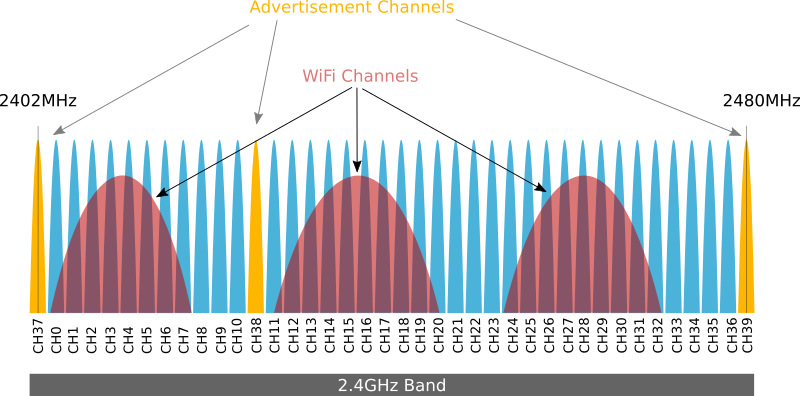
\includegraphics[width=0.7\textwidth]{img/banda-2-4.png}
	\end{center}
	\legend{Fonte: \cite{ble-packets}}
\end{figure}

Interessante notar que esses canais estão posicionados em forma bastante estratégica, no começo, final e meio da banda de 2.4 GHz, com a finalidade de aumentar a eficácia, evitando todos os canais ficarem lotados ou com muita interferência. \cite{ble-packets}. 

Os \textit{BLE Advertisement Packets}, ou pacotes de anúncio \textit{BLE} é uma das formas de conexão do \textit{Bluetooth Smart}. Por meio dos anúncios, um \textit{device} transmite pacotes para todos que estão a sua volta, sem necessariamente necessitar de uma conexão direta entre somente outro dispositivo.

Um \textit{BLE Advertisement Packet} é formado conforme \autoref{fig:ble-adv-packet}. O preâmbulo, \textit{access address} e CRC são informações para formação do pacote. Os dados estão de fato dentro do PDU (\textit{Packet Data Unit}). O cabeçalho de 2 bytes informa o tamanho do \textit{payload} (carga de dados), além de informações relevantes como tipo do pacote, tipo de mensagem enviada, entre outros. \cite{ble-packets}.

\begin{figure}[htb]
	\caption{\label{fig:ble-adv-packet}Modelo de \textit{BLE Advertising Packet}.}
	\begin{center}
		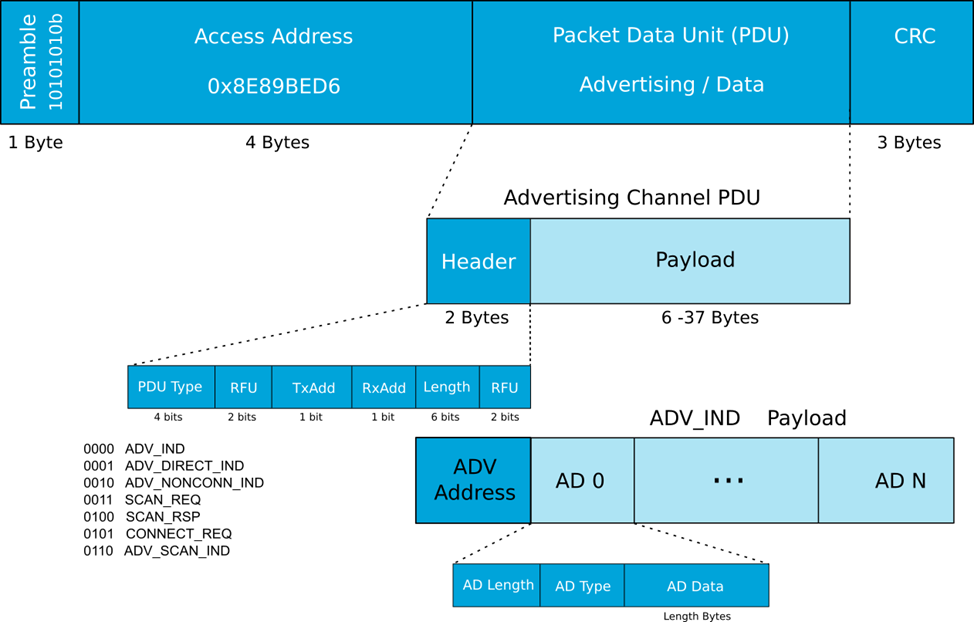
\includegraphics[width=0.8\textwidth]{img/ble-adv-packet.png}
	\end{center}
	\legend{Fonte: \cite{ble-packets}}
\end{figure}

O importante do \textit{BLE Advertising Packet} é o tipo de anúncio feito, ou quais são as informações do pacote. \citeonline{gap-ble} apresenta uma tabela com os possíveis valores e também o significado de cada uma. Por exemplo, o valor 0xFF significa que o pacote contém dados específicos do fabricante, ou seja, existe a flexibilidade de manipular o pacote da forma que for precisa, contanto que mantenha a estrutura original de 6 a 37 bytes de \textit{payload}, conforme \autoref{fig:ble-adv-packet}. \cite{ble-packets}.

% ---
\section{Beacon}\label{sec:beacon}
% ---

Os \textit{beacons} são pequenos sensores que são capazes de identificar objetos com precisão dentro de ambientes fechados. \cite{teixeira-beacon}.

\begin{citacao}
Como muitos espaços fechados (restaurantes, museus, shopping centers, casas de show) possuem estrutura metálica ou utilizam algum tipo de metal em sua construção, é comum que o sinal de GPS fique enfraquecido quando os usuários estão dentro daquele local. Nesse caso, os \textit{Beacons} são uma ótima solução: um hardware relativamente barato, e pequeno o suficiente para ser plugado na parede ou instalado sobre um balcão. \cite{teixeira-beacon}.
\end{citacao}

\begin{figure}[htb]
	\caption{\label{fig:beacon-mpact}Modelo de \textit{beacon} proprietário: MPact, da Zebra Technologies Corporation.}
	\begin{center}
		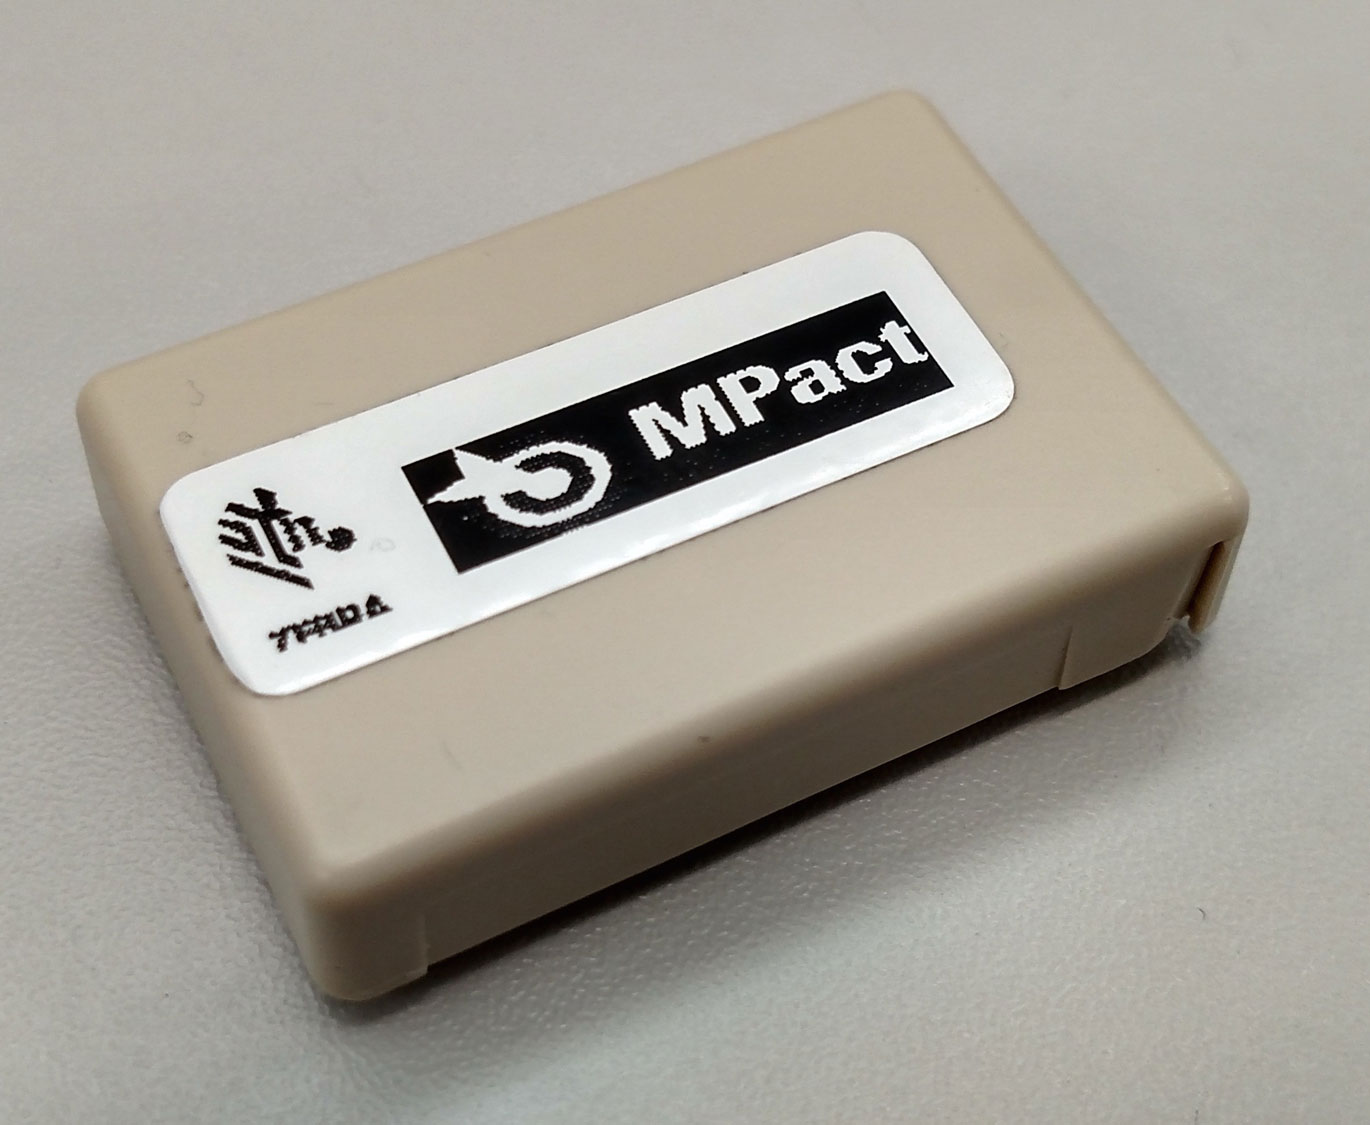
\includegraphics[width=0.6\textwidth]{img/beacon-mpact.jpg}
	\end{center}
	\legend{Fonte: elaborado pelo autor}
\end{figure}

Segundo \citeonline{teixeira-beacon}, os \textit{beacons} utilizam o \textit{BLE} para detectar um dispositivo próximo e transmitir seu identificador único e avisar que está ali presente. \citeonline{teixeira-beacon} também diz que os \textit{beacons} não são inteligentes, toda a interação deve depender do dispositivo que recebe a informação do identificador único.

Atualmente os usos de \textit{beacons} estão restritos a aplicativos em smartphones realizando a leitura e interagindo com o usuário, porém existem ainda diversas áreas a serem exploradas, e um bom exemplo são as casas inteligentes. Segundo \citeonline{grothaus-smarthomes}, a \textit{Apple} está apostando em um kit de desenvolvimento (\textit{HomeKit}) que permita aos desenvolvedores interagirem com \textit{smart devices} presentes no ambiente.

% ---
\subsection{\textit{iBeacon}}\label{sec:ibeacon}
% ---

O protocolo \textit{iBeacon} foi apresentado pela Apple juntamente com o iOS 7, versão de seu sistema operacional para dispositivos móveis. É uma tecnologia baseada nos \textit{beacons}, porém adaptada para as necessidades e aplicações de seu sistema móvel.

A Apple adaptou o pacote genérico de \textit{beacon} para transmitir três dados:

\begin{alineas}
	\item \textbf{UUID}: Identificador único formado de 16 bytes (128 bits). Focado em ser único para cada aplicação. Cada aplicação deve ter um único UUID.
	\item \textbf{\textit{Major}}: Identificador de 2 bytes que identifica uma sub-região grande. Usado, por exemplo, para dividir as lojas de um grande varejista.
	\item \textbf{\textit{Minor}}: Identificador de 2 bytes que identifica uma sub-divisão de região, ou seja, uma região menor que o Major.
\end{alineas}

Um exemplo de aplicação é citado na \autoref{table:stores-apple}. Utiliza-se um único UUID para todas as lojas, um número \textit{Major} por loja e um \textit{Minor} por departamento, podendo este último ser repetido entre as lojas.

\begin{table}[htb]
	\IBGEtab{%
  		\caption{Exemplo de aplicação}%
  		\label{table:stores-apple}
	}{%
  		\begin{tabular}{cccc}
	  		\toprule
	 			Localização da Loja & São Francisco & Paris & Londres \\
  			\midrule
				UUID & \multicolumn{3}{c}{D9B9EC1F-3925-43D0-80A9-1E39D4CEA95C} \\
			\midrule
				\textit{Major} & 1 & 2 & 3 \\
			\midrule 
				\textit{Minor} (Roupas) & 10 & 10 & 10 \\
  			\midrule 
				\textit{Minor} (Utilidades Domésticas) & 20 & 20 & 20 \\
			\midrule 
				\textit{Minor} (Automotivo) & 30 & 30 & 30 \\
  			\bottomrule
		\end{tabular}%
	}{%
  		\fonte{\cite{ibeacon-apple}}%
  	}
\end{table}

O pacote \textit{BLE} utilizado pela tecnologia iBeacon pode ser visto na \autoref{fig:ibeacon-packet}. Segundo \citeonline{arm-beacons}, o prefixo determinado para o protocolo \textit{iBeacon} é:

\begin{alineas}
	\item \textit{\textbf{Adv Flags}}: determinam que é um pacote \textit{BLE} de descobrimento geral, e que somente transmite e não permite conexões.
	\item \textit{\textbf{Adv Header}}: determinam que os próximos 26 bytes serão a carga de dados (\textit{payload} de fato). Sempre será 0x1AFF.
	\item \textit{\textbf{Company ID}}: indica que é o ID da Apple junto com a Bluetooth SIG. Essa informação que faz ser dependente da Apple. Sempre será 0x004C.
	\item\textit{\textbf{iBeacon Type}}: ID secundário utilizado por todos iBeacons que identificam ser um \textit{beacon} de proximidade. Sempre será 0x02.
	\item\textit{\textbf{iBeacon Length}}: identifica quantos bytes terão em seguida. Sempre será 0x15, ou 21 bytes.
\end{alineas}

\begin{figure}[htb]
	\caption{\label{fig:ibeacon-packet}\textit{Payload} do pacote iBeacon.}
	\begin{center}
		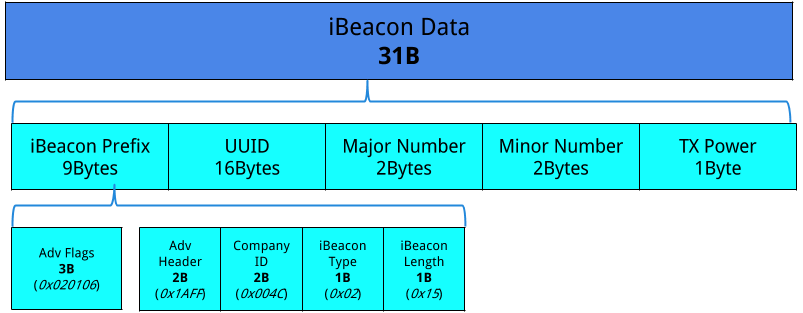
\includegraphics[width=0.9\textwidth]{img/ibeacon-packet.png}
	\end{center}
	\legend{Fonte: \cite{arm-beacons}}
\end{figure}

Os \textit{iBeacons} foram criados com intuito de serem descobertos por smartphones. Um exemplo de aplicação é uma cafeteria com um \textit{iBeacon} no balcão próximo ao caixa. Quando um consumidor entra na loja e chega próximo ao caixa, um aplicativo em seu celular identifica o \textit{iBeacon} pela sua UUID, identifica pelo \textit{Major} que se trata da cafeteria número 12 e encontra uma promoção com o \textit{Minor} de número 26. Em seguida, apresenta uma notificação ao usuário uma promoção e também um cupom válido de desconto para usar no caixa. \cite{arm-beacons}.

Uma outra aplicação interessante citada por \citeonline{arm-beacons} é a possibilidade do smartphone transmitir pacotes \textit{iBeacon}, sem necessidade de um hardware externo. Dessa forma, pode-se por exemplo automatizar o check-in em um evento e rastrear o movimento dos usuários entre os estabelecimentos.

% ---
\subsection{Outros Protocolos}\label{sec:outros-protocolos}
% ---

Existem mais protocolos baseados na tecnologia \textit{beacon}. Dois se destacam por ser abertos e passíveis de alterações: \textit{AltBeacon} e \textit{Eddystone}, este último criado pela Google. O \textit{AltBeacon} possui um modelo bastante parecido com o \textit{iBeacon}, porém com possibilidade de alterar o número do fabricante, ter possibilidade de código de \textit{beacons} diferentes, e também a possibilidade do fabricante colocar sua informação ao final do pacote, conforme \autoref{fig:altbeacon-packet} \cite{arm-beacons}.

\begin{figure}[htb]
	\caption{\label{fig:altbeacon-packet}Pacote do \textit{AltBeacon}.}
	\begin{center}
		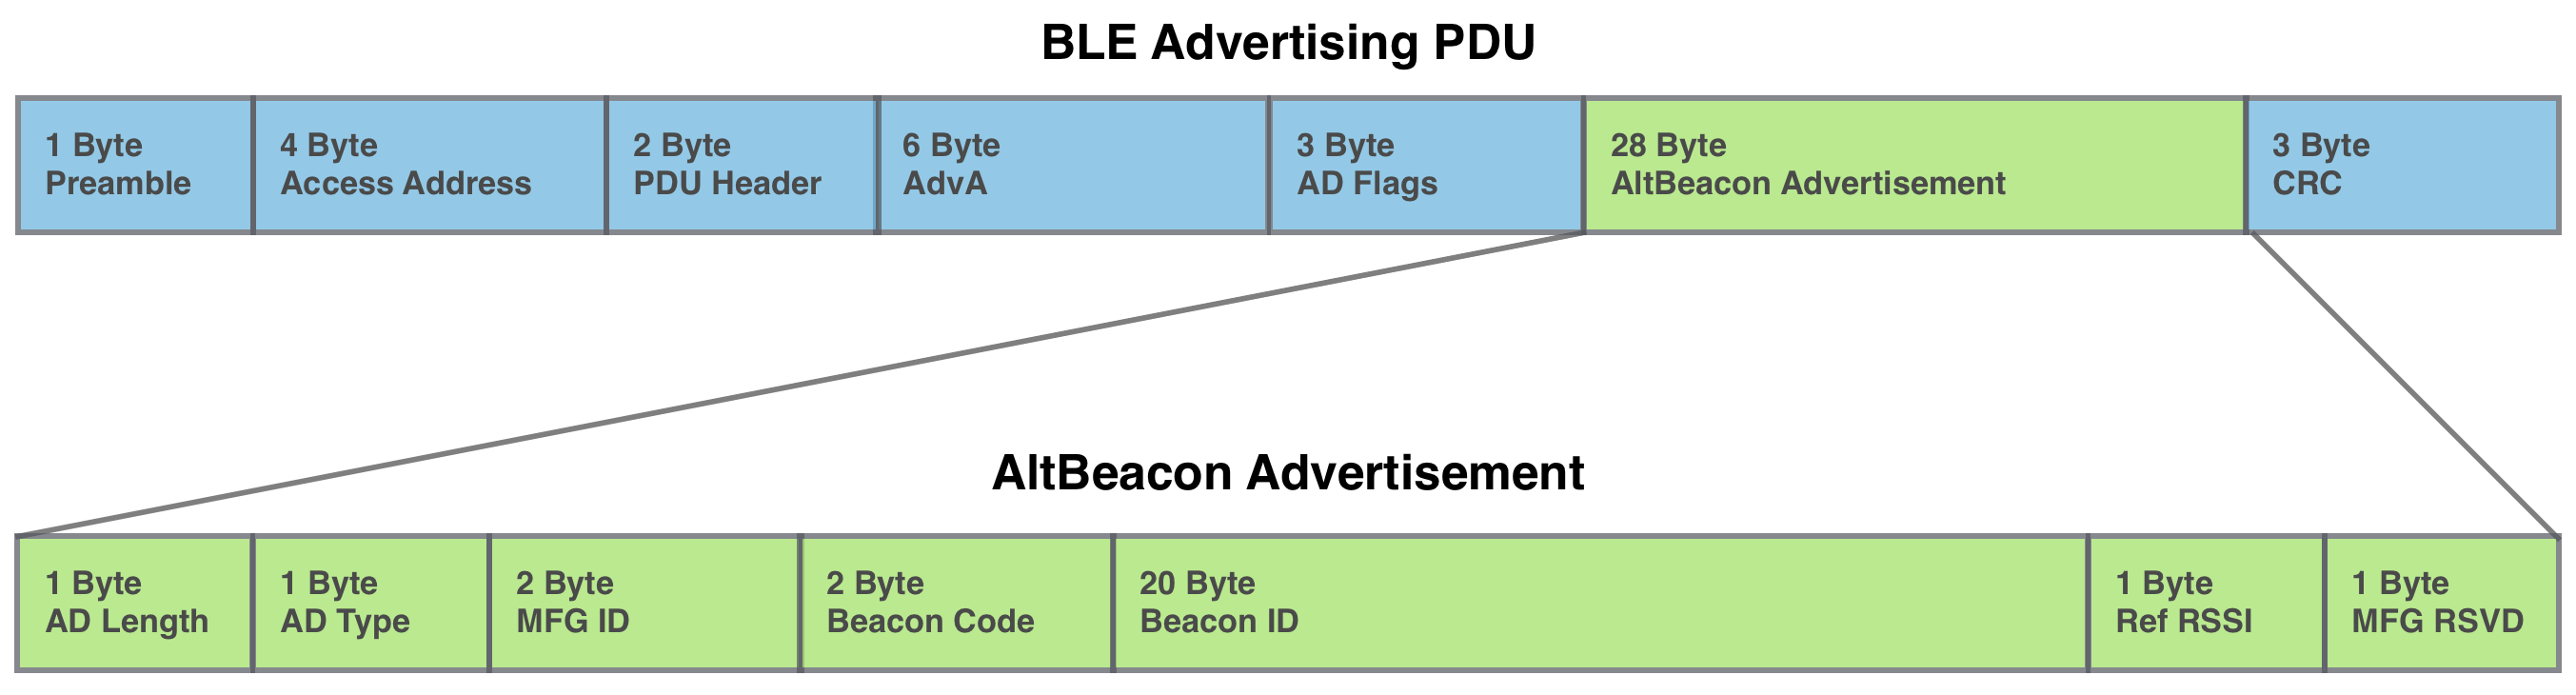
\includegraphics[width=1\textwidth]{img/altbeacon-packet.png}
	\end{center}
	\legend{Fonte: \cite{arm-beacons}}
\end{figure}

Segundo \citeonline{eddystone-google}, o protocolo \textit{Eddystone} possui três modos de funcionamento:
\begin{alineas}
	\item \textit{Eddystone}-UID: transmite um \textit{beacon} ID, composto de 10 bytes identificando um grupo de \textit{beacons} e  6 bytes identificando um único \textit{beacon}.
	\item \textit{Eddystone}-URL: transmite um link comprimido, para que o cliente possa acessar um site na internet.
	\item \textit{Eddystone}-TLM: transmite informações de telemetria sobre o \textit{beacon}, como por exemplo voltagem da bateria, temperatura e quantos pacotes foram enviados.
\end{alineas}

% ----------------------------------------------------------

% ----------------------------------------------------------


% ----------------------------------------------------------
% Materiais e Métodos
% ----------------------------------------------------------
\chapter{Metodologia}\label{cap:metodologia}
% ----------------------------------------------------------

% ----------------------------------------------------------
\section{Métodos e Etapas}\label{sec:metodos-etapas}
% ----------------------------------------------------------

O projeto foi dividido em três etapas para facilitar o desenvolvimento completo. A primeira etapa foi o levantamento bibliográfico relacionado ao tema, realizadas buscas relacionadas aos assuntos: \textit{Raspberry Pi}, comunicação via \textit{Bluetooth Low Energy}, \textit{beacons}. Concomitantemente foi realizado o estudo prático das tecnologias, levando em conta suas capacidades, limitações, e aplicações.

A segunda etapa foi planejar o projeto baseado na análise do levantamento bibliográfico, assim como a definição de sua estrutura. Essa etapa foi necessária para facilitar e agilizar a implementação e testes dos componentes nas próximas etapas, definindo assim um escopo inicial de funcionalidades que o sistema terá, assim como outras tarefas a serem realizadas. O processo está detalhado no \autoref{cap:desenvolvimento} - \nameref{cap:desenvolvimento}.

A terceira etapa foi a implementação e testes do protótipo. As funcionalidades foram divididas em módulos para facilitar os testes e detectar possíveis erros e \textit{bugs}.

Todo o projeto foi desenvolvido no espaço do LTIA\footnote{Laboratório de Tecnologia da Informação Aplicada - \url{http://www.ltia.fc.unesp.br/}}, da Universidade Estadual Paulista "Júlio de Mesquita Filho"\ - Campus Bauru.


% ----------------------------------------------------------
\section{Materiais Utilizados}\label{sec:materiais-utilizados}
% ----------------------------------------------------------

% ---
\subsection{Raspberry Pi e Acessórios}\label{sec:rpi-acessorios}
% ---

A versão do Raspberry Pi escolhida para o projeto foi a 2 Modelo B, por ter mais processamento e mais memória RAM (\autoref{fig:rpi2-utilizado}), conforme informado na \autoref{sec:raspberry-pi}.

É necessário o uso de um adaptador \textit{WiFi} para conexão a internet sem necessidade de cabo \textit{Ethernet} e também um adaptador Bluetooth 4.0 com suporte a \textit{BLE} para fazer a busca dos pacotes \textit{beacon}. Os modelos de adaptadores usados foram Orico BTA-406 (bluetooth) e EDUP N8508GS (\textit{WiFi}), conforme \autoref{fig:adaptadores}. O \textit{RPi} e os adaptadores são de propriedade do autor.

O sistema operacional executado no RPi foi instalado em um cartão microSD, com no mínimo 4 GB de espaço. O cartão utilizado nesse projeto foi um SanDisk Ultra Class 10 de 8 GB. 

O sistema utilizado foi o Raspbian Wheezy. Durante o desenvolvimento do projeto, a versão Raspbian Jessie foi lançada, com inúmeras melhorias, porém preferiu-se por permanecer na versão Wheezy para evitar possíveis incompatibilidades com os softwares utilizados.

\begin{figure}[htb]
	\caption{\label{fig:rpi2-utilizado}\textit{RPi} 2 modelo B utilizado nesse projeto.}
	\begin{center}
		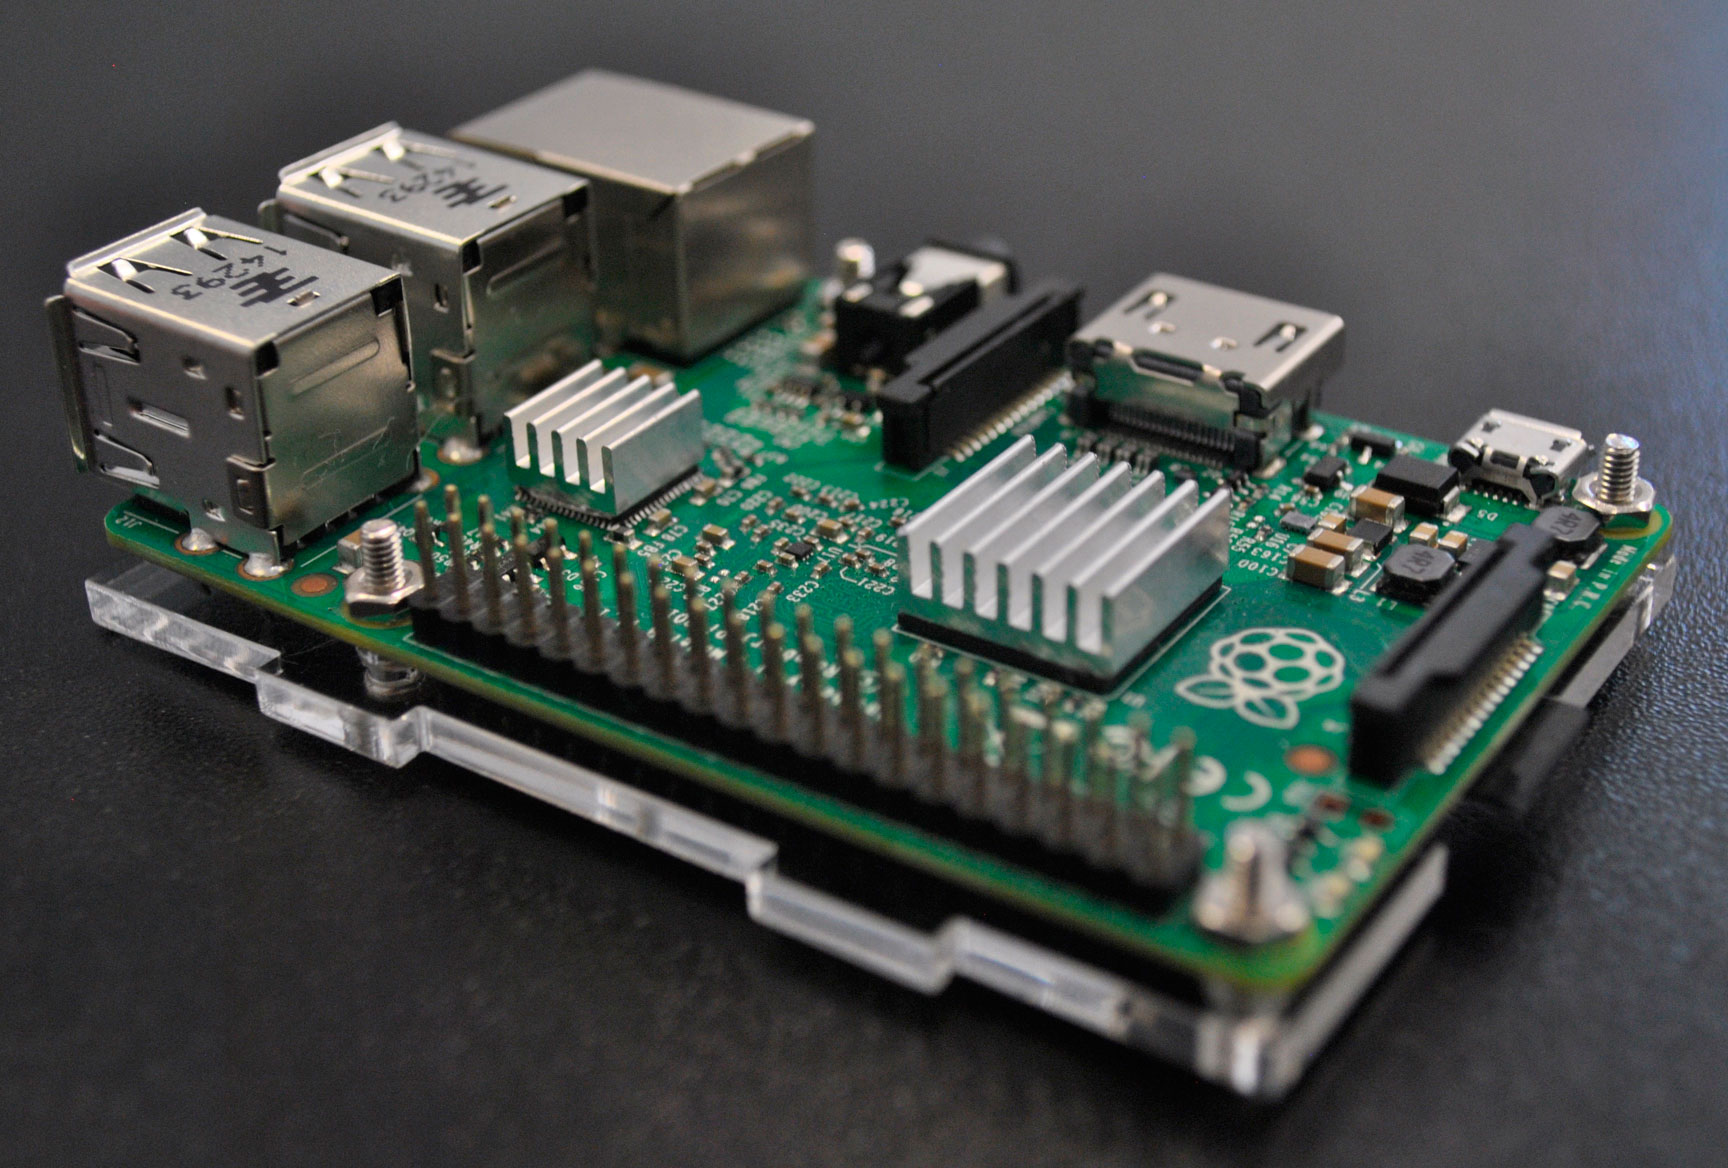
\includegraphics[width=0.7\textwidth]{img/rpi2.jpg}
	\end{center}
	\legend{Fonte: elaborado pelo autor}
\end{figure}

\begin{figure}[htb]
	\caption{\label{fig:adaptadores}Orico BTA-406 a esquerda e EDUP N8508GS a direita.}
	\begin{center}
		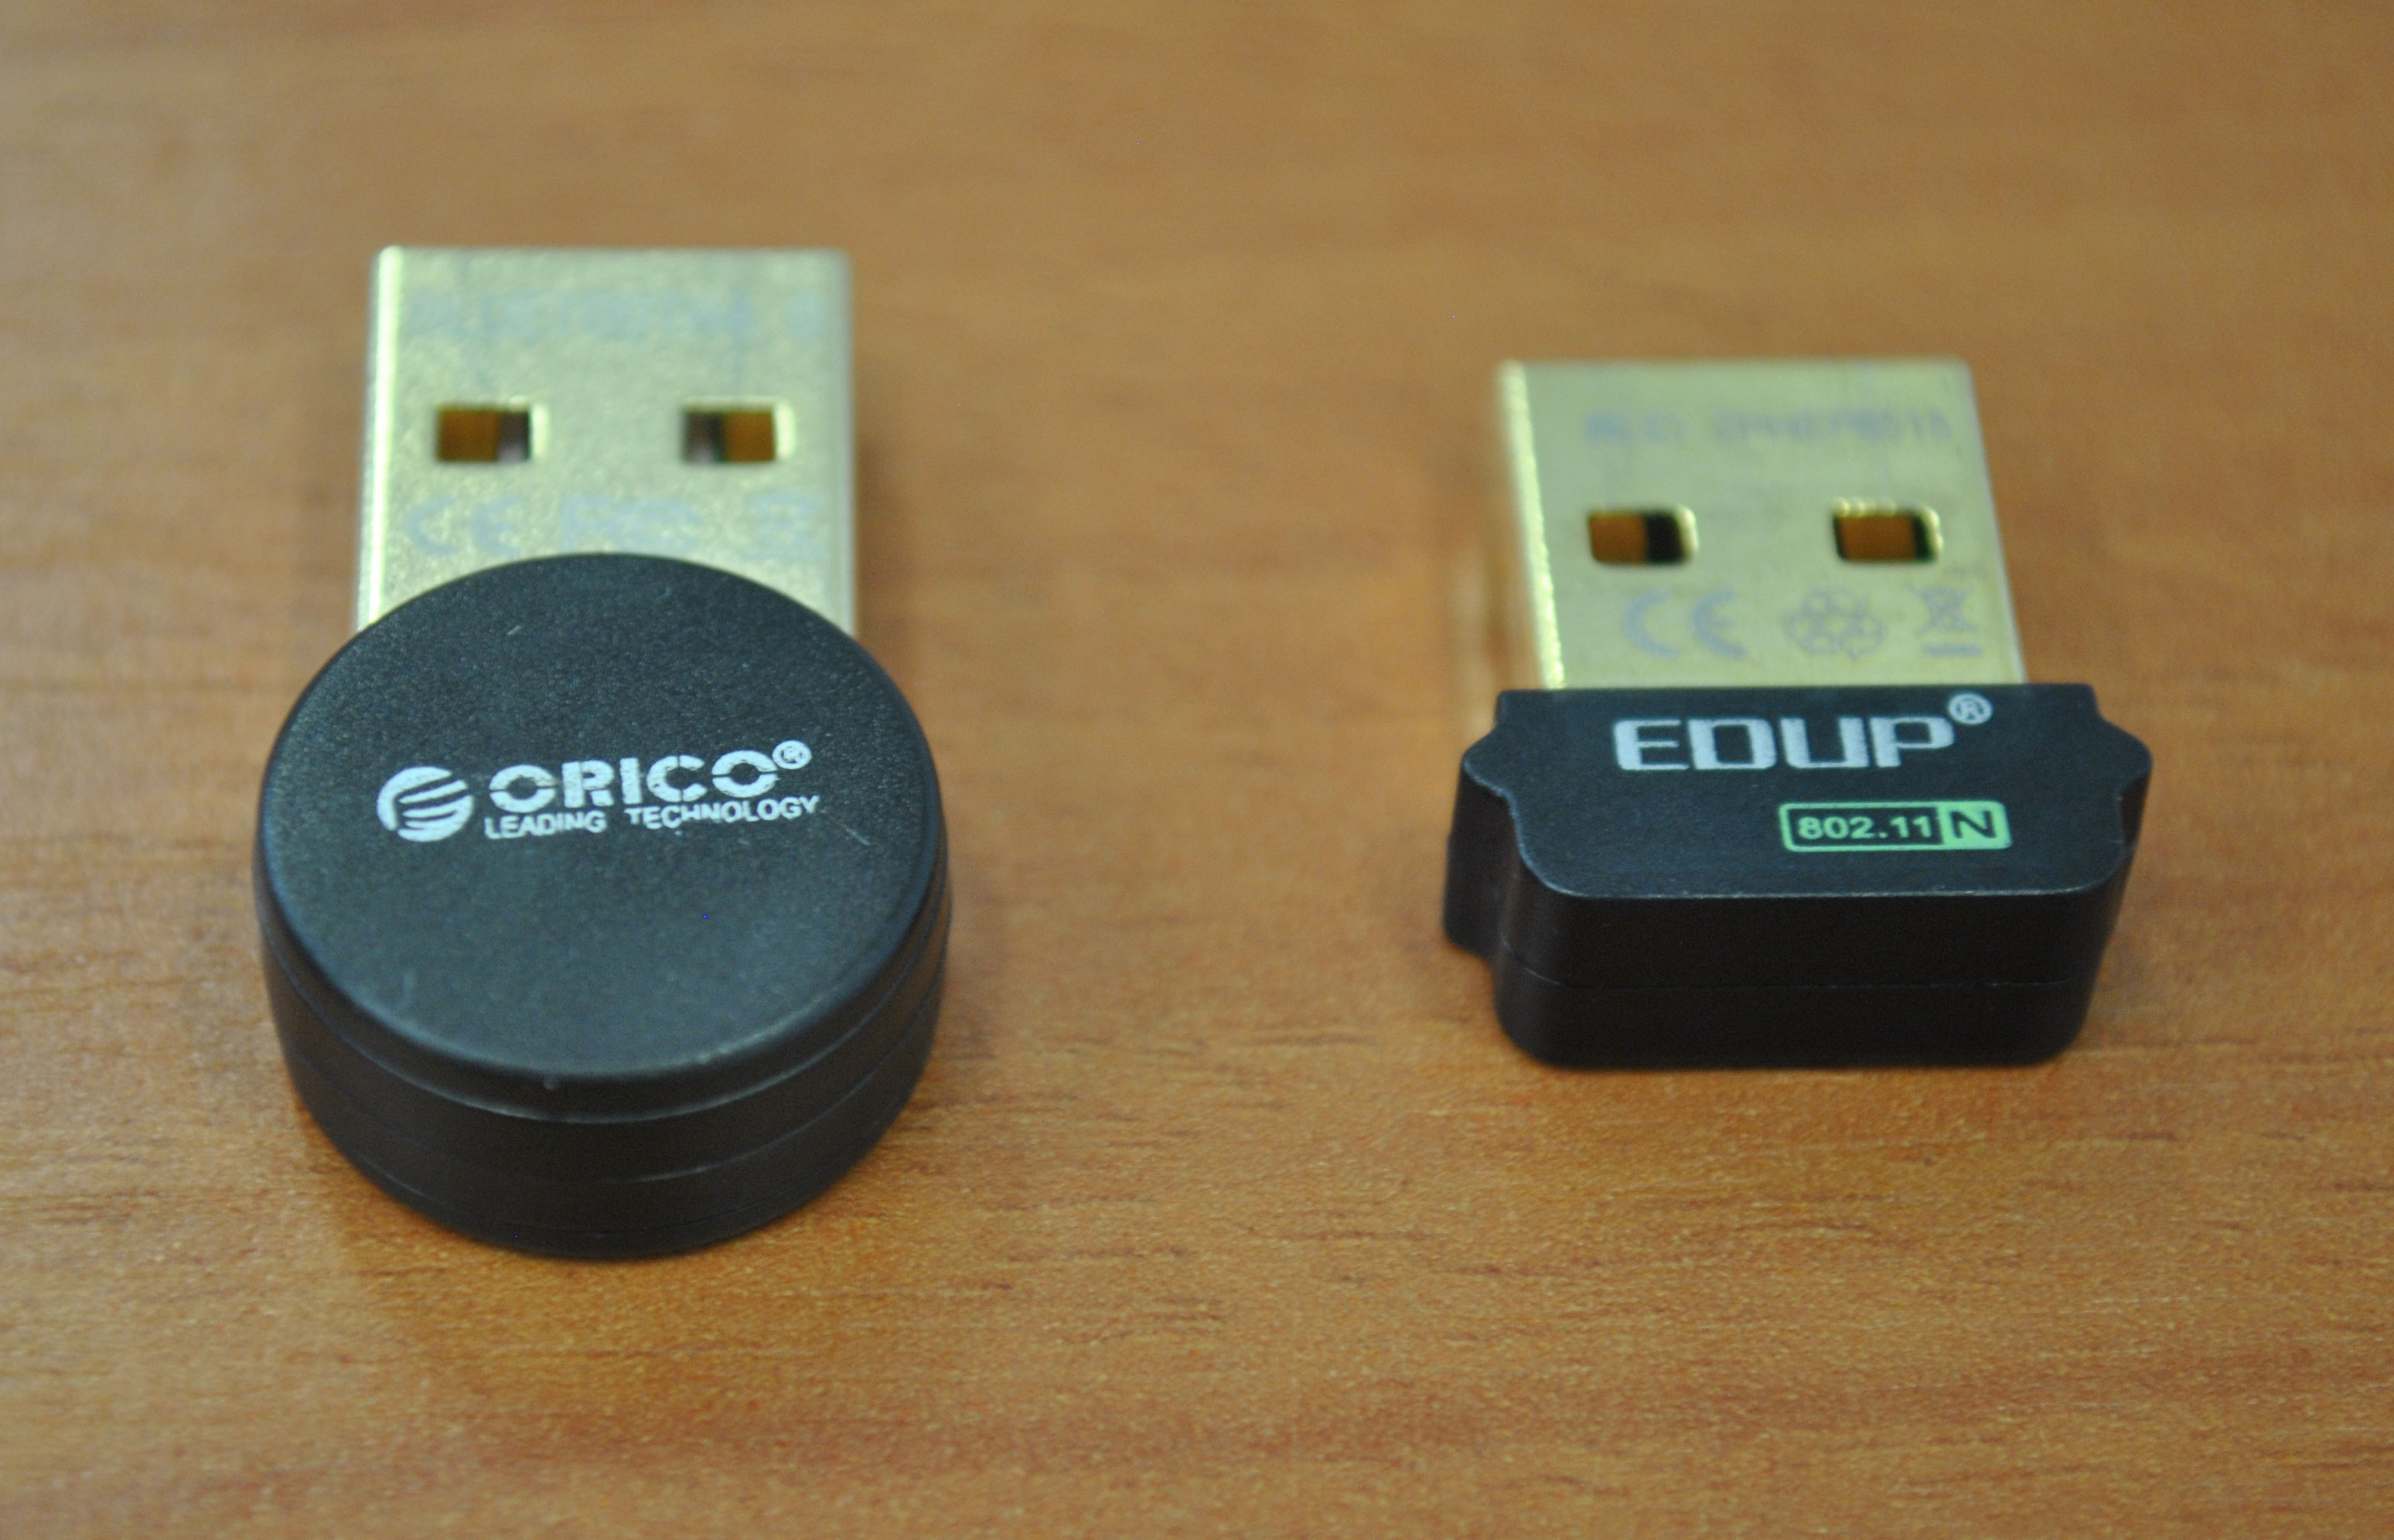
\includegraphics[width=0.5\textwidth]{img/adaptadores.jpg}
	\end{center}
	\legend{Fonte: elaborado pelo autor}
\end{figure}

Na \autoref{sec:tecnologias-ferramentas} - \nameref{sec:tecnologias-ferramentas}, \autoref{sec:rpi-tecnologia} - \nameref{sec:rpi-tecnologia} aborda-se como o \textit{RPi} funciona na prática, como foi utilizado para esse projeto e como suas capacidades foram aproveitadas.

% ---
\subsection{Computadores e Softwares}\label{sec:comp-softwares}
% ---

A conexão com o \textit{RPi} foi realizada utilizando \textit{SSH}\footnote{\textit{Secure Shell}}, sem necessidade de monitor e teclado. O computador utilizado no projeto foi um MacBook Pro com sistema Mac OS X 10.10, posteriormente atualizado para 10.11. 

Nesse sistema o uso de \textit{SSH} é simples, basta abrir o aplicativo Terminal e utilizar o comando "\textit{ssh usuario@computador}", conforme \autoref{fig:ex-terminal}. Esse tipo de abordagem é bastante utilizada para conexão a servidores na nuvem, para executar comandos, softwares, entre outros.

\begin{figure}[htb]
	\caption{\label{fig:ex-terminal}Conexão com o \textit{RPi} via \textit{SSH}.}
	\begin{center}
		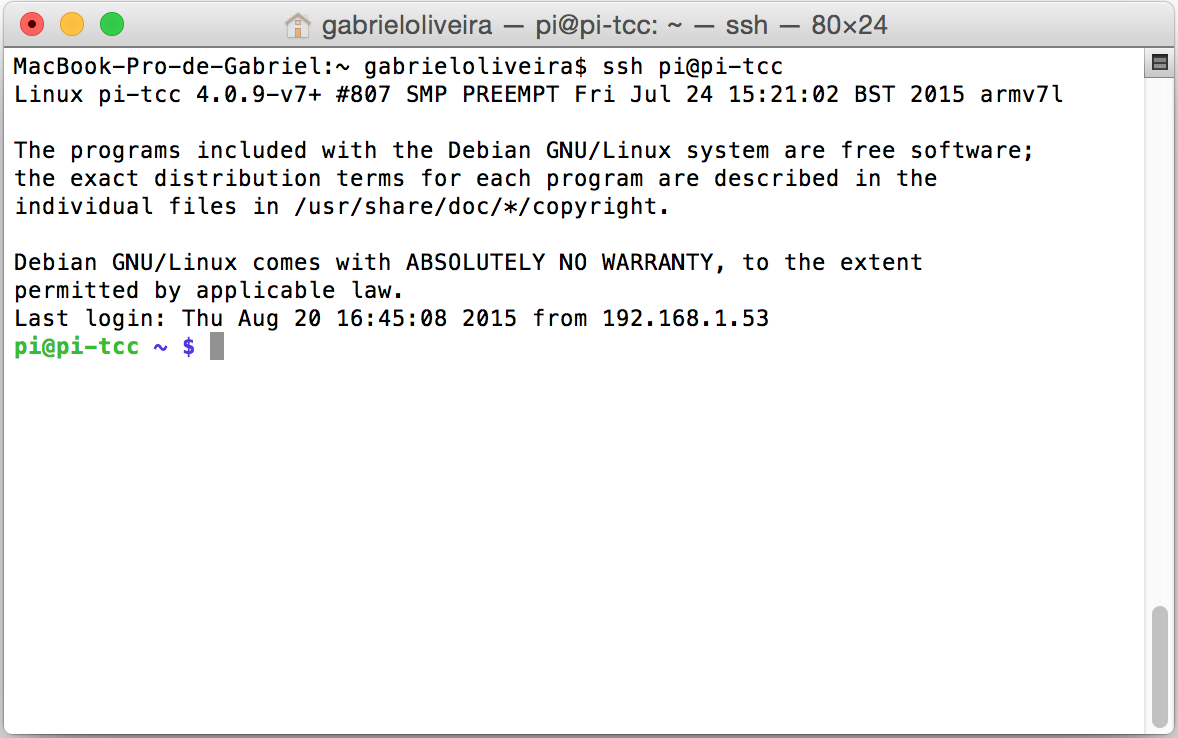
\includegraphics[width=0.9\textwidth]{img/terminal-pi.png}
	\end{center}
	\legend{Fonte: elaborado pelo autor}
\end{figure}

% ---
\subsection{Smartphones e Tablets}\label{sec:smartphone-tablets}
% ---

Foi utilizado o smartphone Moto Maxx com sistema Android 5.0.1 e o tablet iPad mini Retina com sistema iOS 8.4 confirme \autoref{fig:motomaxx-ipad}. 

O aplicativo utilizado em ambos foi o \textit{Locate Beacon} da \textit{Radius Networks}, que nos permite identificar os \textit{beacons} e também simular um, para realizar os testes com diferentes tipos, podendo alterar os valores de UUID, Major, Minor e potência de transmissão. 

\begin{figure}[htb]
	\caption{\label{fig:motomaxx-ipad}Moto Maxx (esquerda) e iPad Mini (direita).}
	\begin{center}
		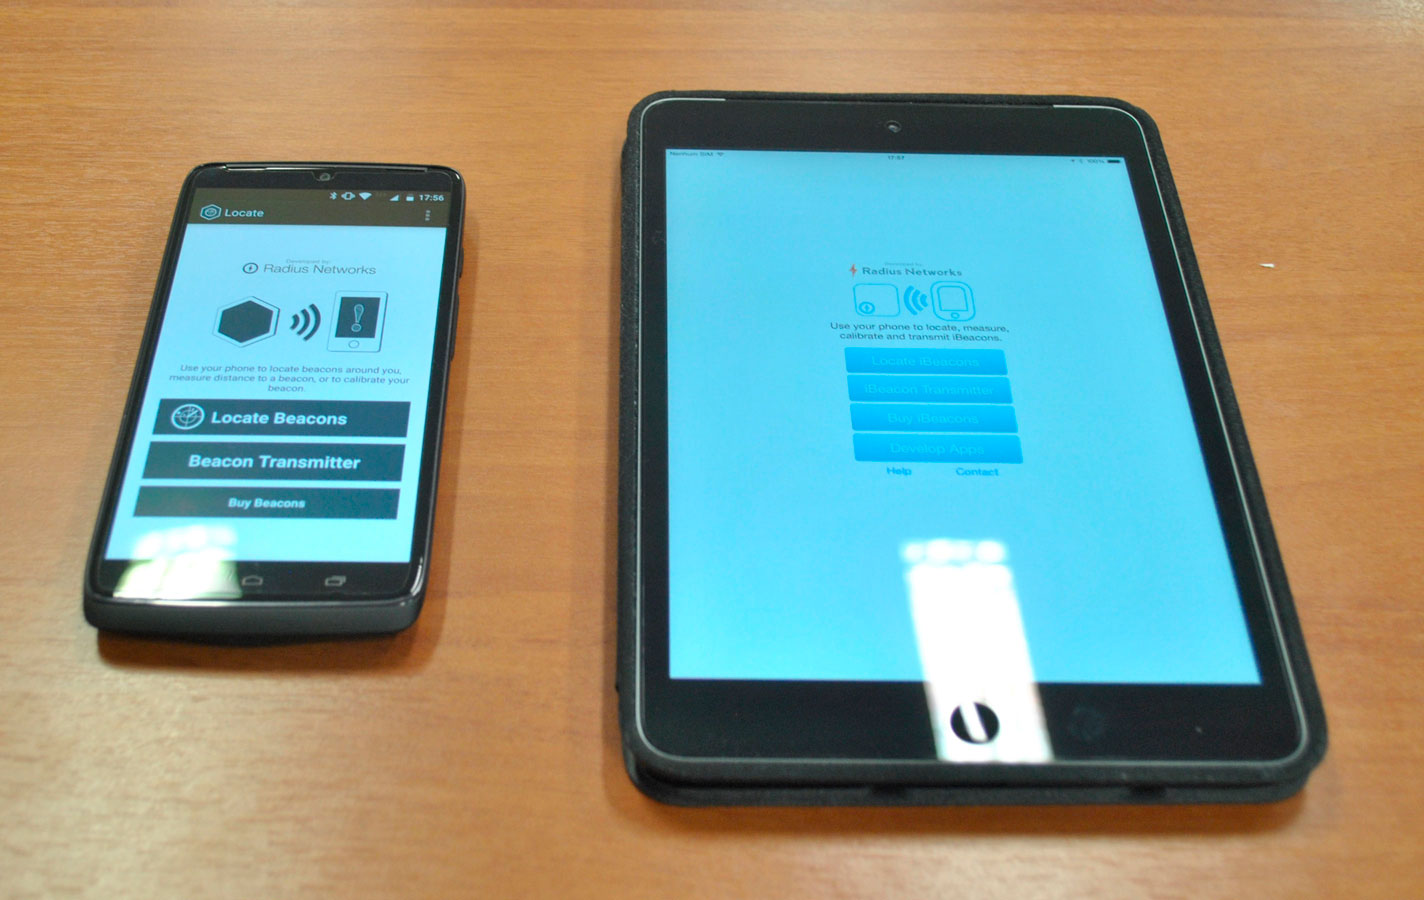
\includegraphics[width=0.7\textwidth]{img/motomaxx-ipad.jpg}
	\end{center}
	\legend{Fonte: elaborado pelo autor}
\end{figure}

% ---
\subsection{Beacons}\label{sec:beacons-modo}
% ---

O \textit{beacon} utilizado para testes foi o \textit{Zebra MPact}, conforme \autoref{fig:zebra-mpact}. Utiliza uma bateria CR2450 para alimentação de energia. 

\begin{figure}[htb]
	\caption{\label{fig:zebra-mpact}\textit{Beacon} Zebra MPact utilizado para testes.}
	\begin{center}
		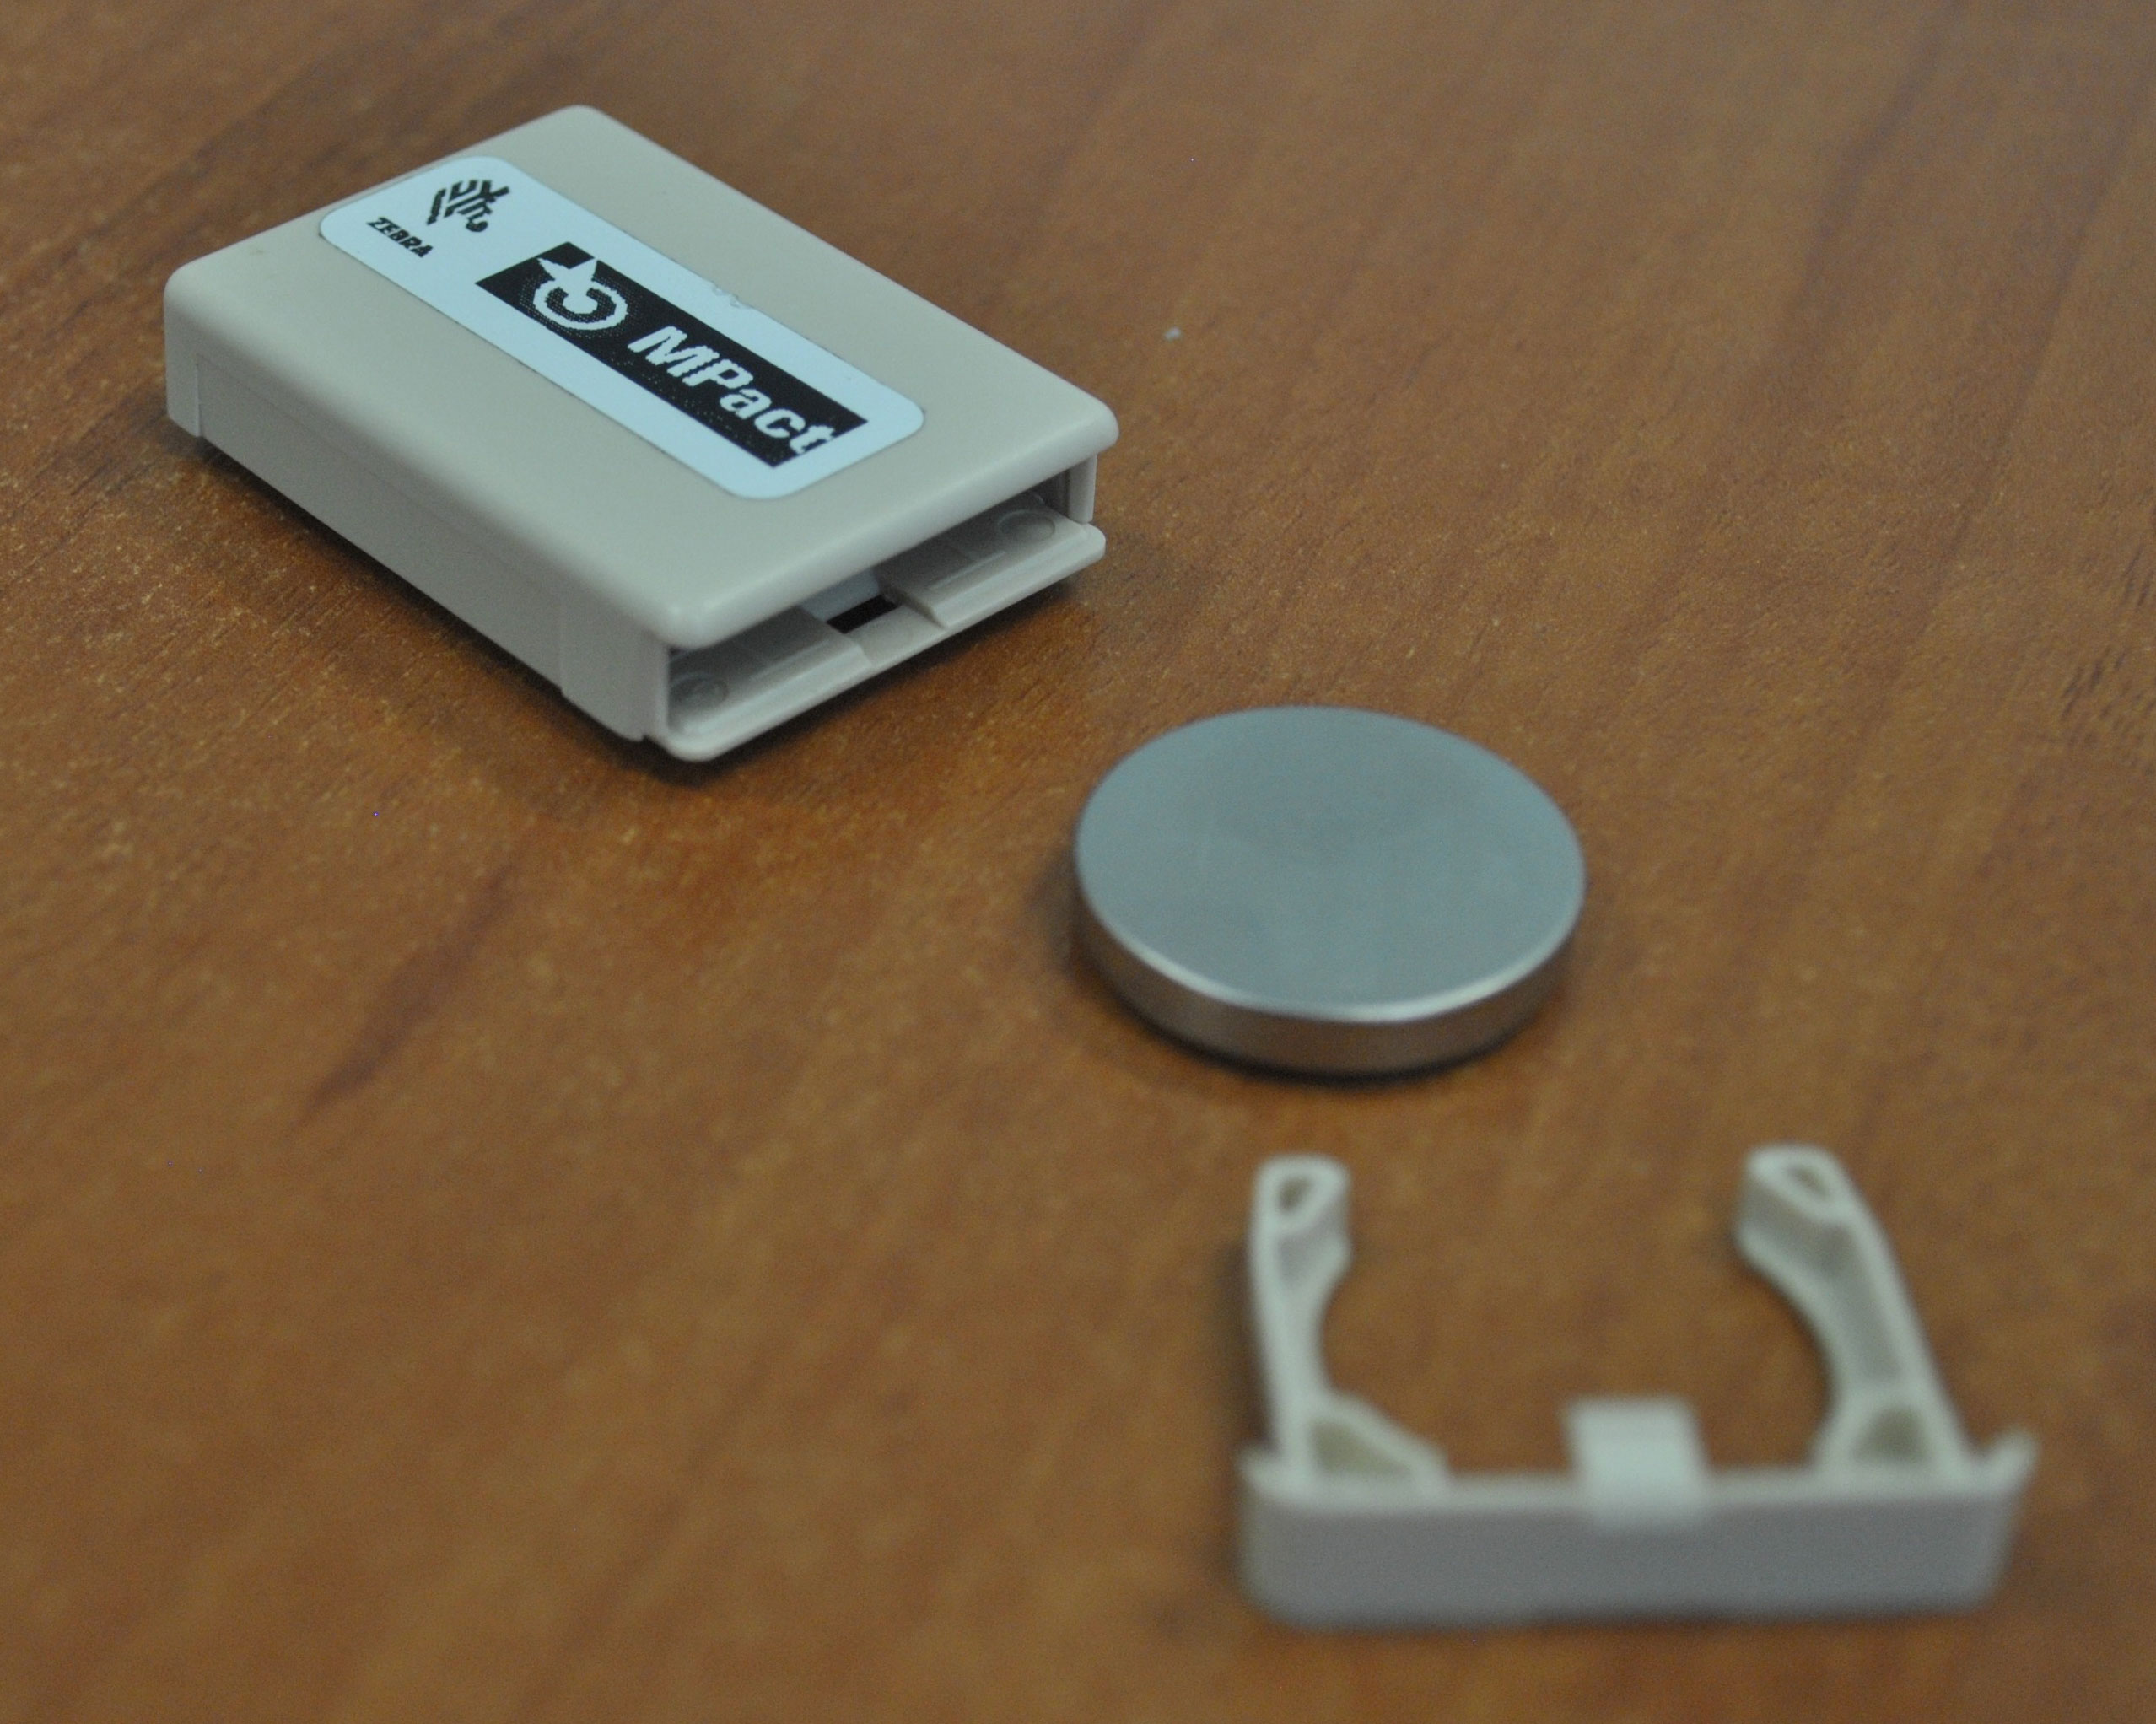
\includegraphics[width=0.6\textwidth]{img/beacon-mpact2.jpg}
	\end{center}
	\legend{Fonte: elaborado pelo autor}
\end{figure}

A empresa \textit{Zebra} tem um sistema de administração e gerenciamento nomeado \textit{MPact Toolbox}, instalado em um servidor do LTIA com sistema Debian 8.1. Esse sistema foi utilizado neste projeto somente para conhecimento da tecnologia \textit{beacon} e atualização do \textit{firmware}, disponível somente via \textit{Toolbox}. Esse software também apresenta a porcentagem de bateria, conforme \autoref{fig:exemplo-toolbox}. 

Permite a configuração de vários \textit{beacons} simultaneamente, além de alterar o modo de funcionamento, de \textit{iBeacon} para \textit{MPact}, protocolo criado pela fabricante.

\begin{figure}[htb]
	\caption{\label{fig:exemplo-toolbox}\textit{Beacon} configurado na \textit{Toolbox} apresentando a porcentagem de bateria.}
	\begin{center}
		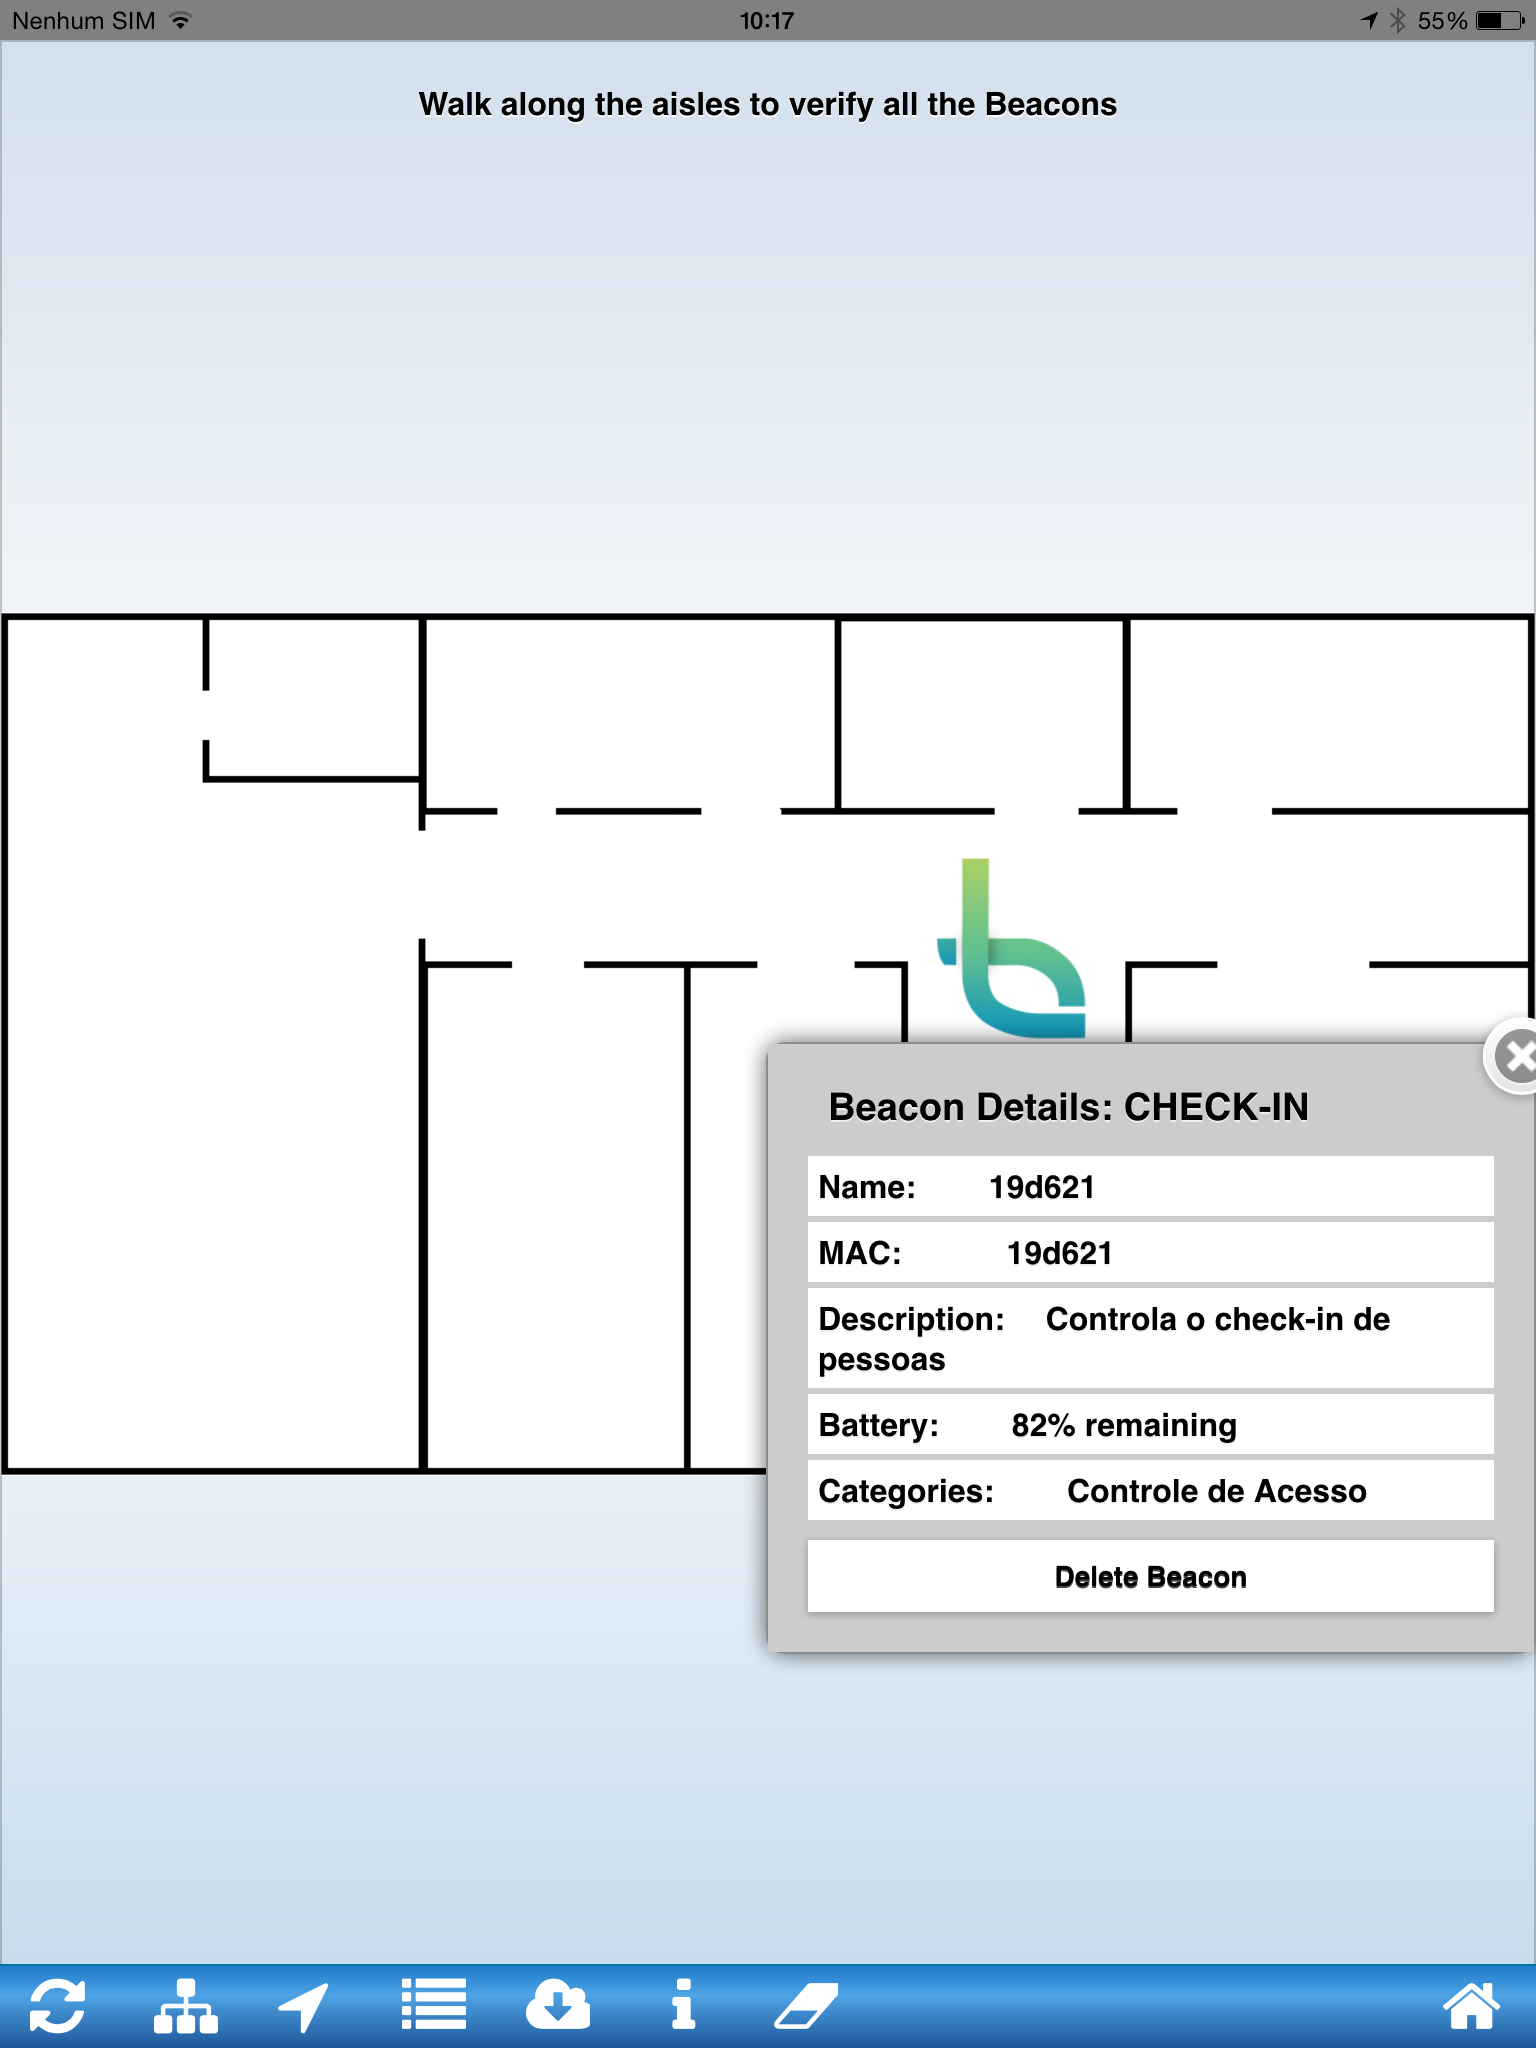
\includegraphics[width=0.7\textwidth]{img/toolbox-exemplo.png}
	\end{center}
	\legend{Fonte: elaborado pelo autor}
\end{figure}

% ---
\subsection{Acessórios para o Protótipo}\label{sec:acess-prototipo}
% ---

O protótipo foi adaptado em uma caixa de metal (\autoref{fig:caixa-metal}), furada conforme projeto e pintada de preto. Esse processo está detalhado na \autoref{sec:segunda-etapa}. 

\begin{figure}[htb]
	\caption{\label{fig:caixa-metal}Caixa de metal utilizada para o protótipo}
	\begin{center}
		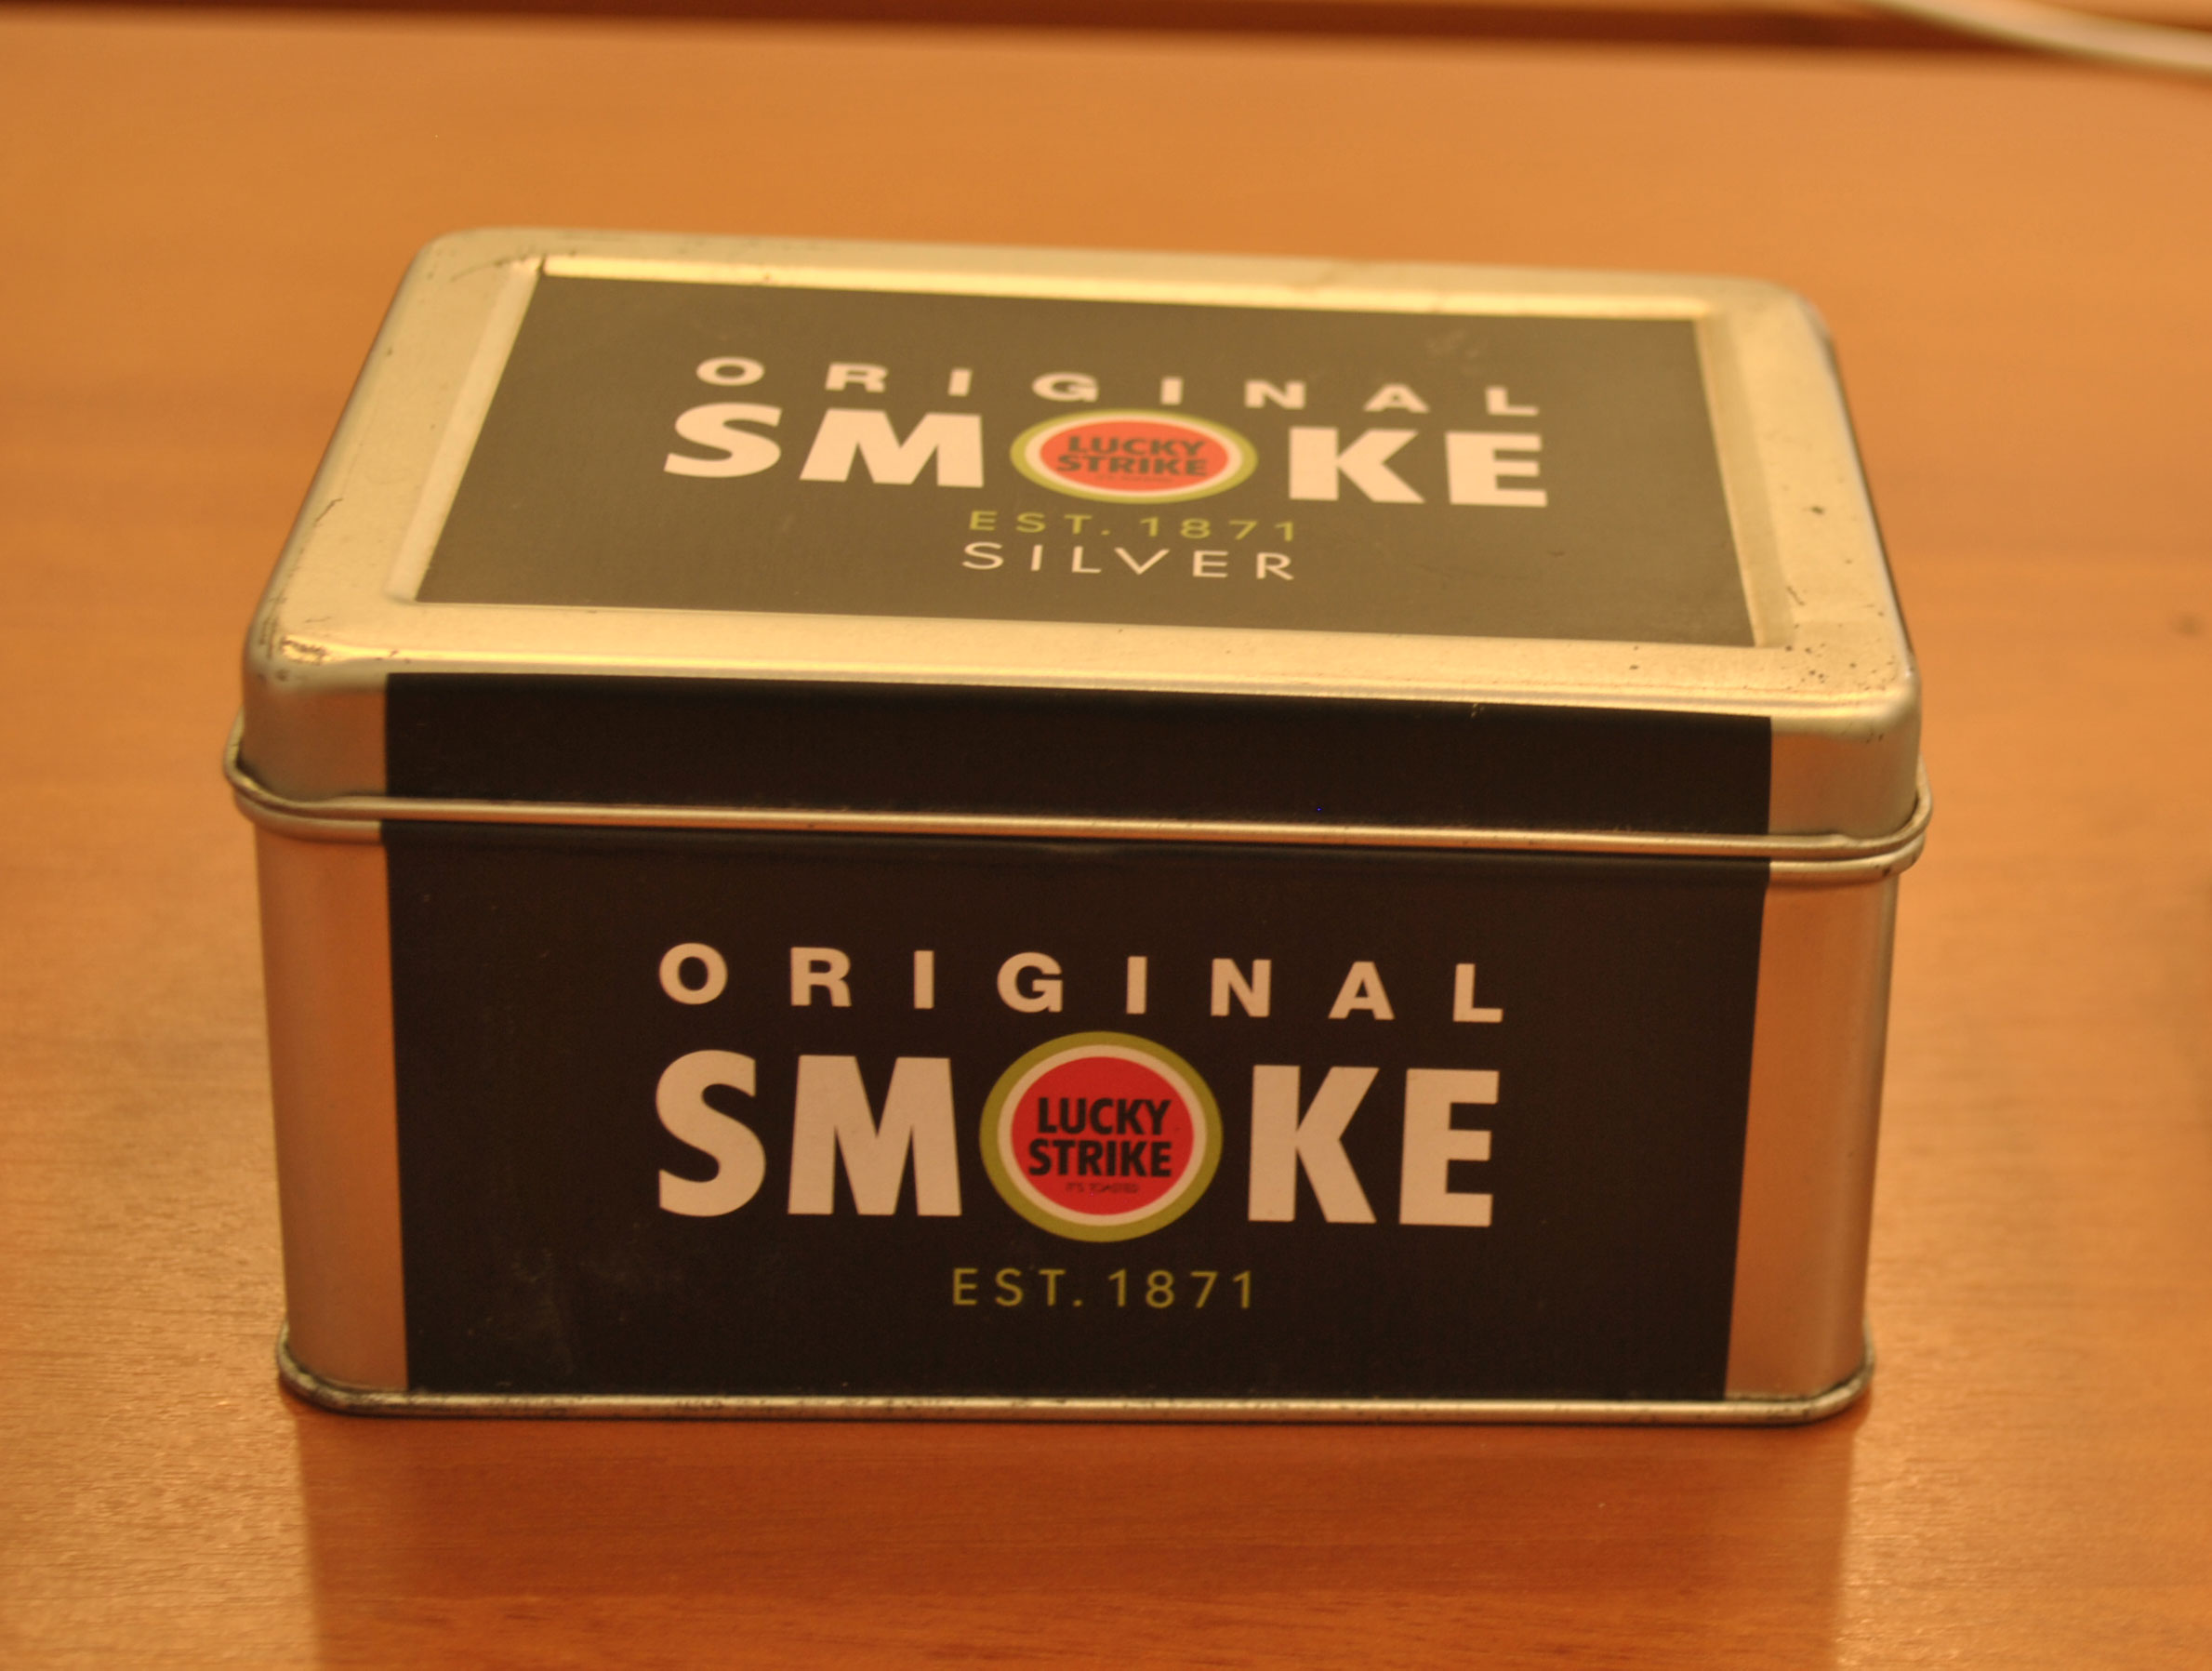
\includegraphics[width=0.7\textwidth]{img/caixa-metal.jpg}
	\end{center}
	\legend{Fonte: elaborado pelo autor}
\end{figure}

Para o protótipo final foram utilizados seis LEDs, resistores, barra de pinos, um display azul de 16 colunas por 2 linhas, três botões do tipo clique, cabos \textit{flat} do tipo IDE e \textit{floppy}, placas com furação para soldagem de componentes, cabos finos removidos de um cabo de rede \textit{ethernet} para ligações entre os componentes e cola quente para fixação dos componentes internos. Esses materiais podem ser vistos na \autoref{fig:prot-interno}.

\begin{figure}[htb]
	\label{teste}
	\centering
 	\begin{minipage}{0.43\textwidth}
		\centering
		\caption{\label{fig:prot-interno}Parte interna do protótipo}
		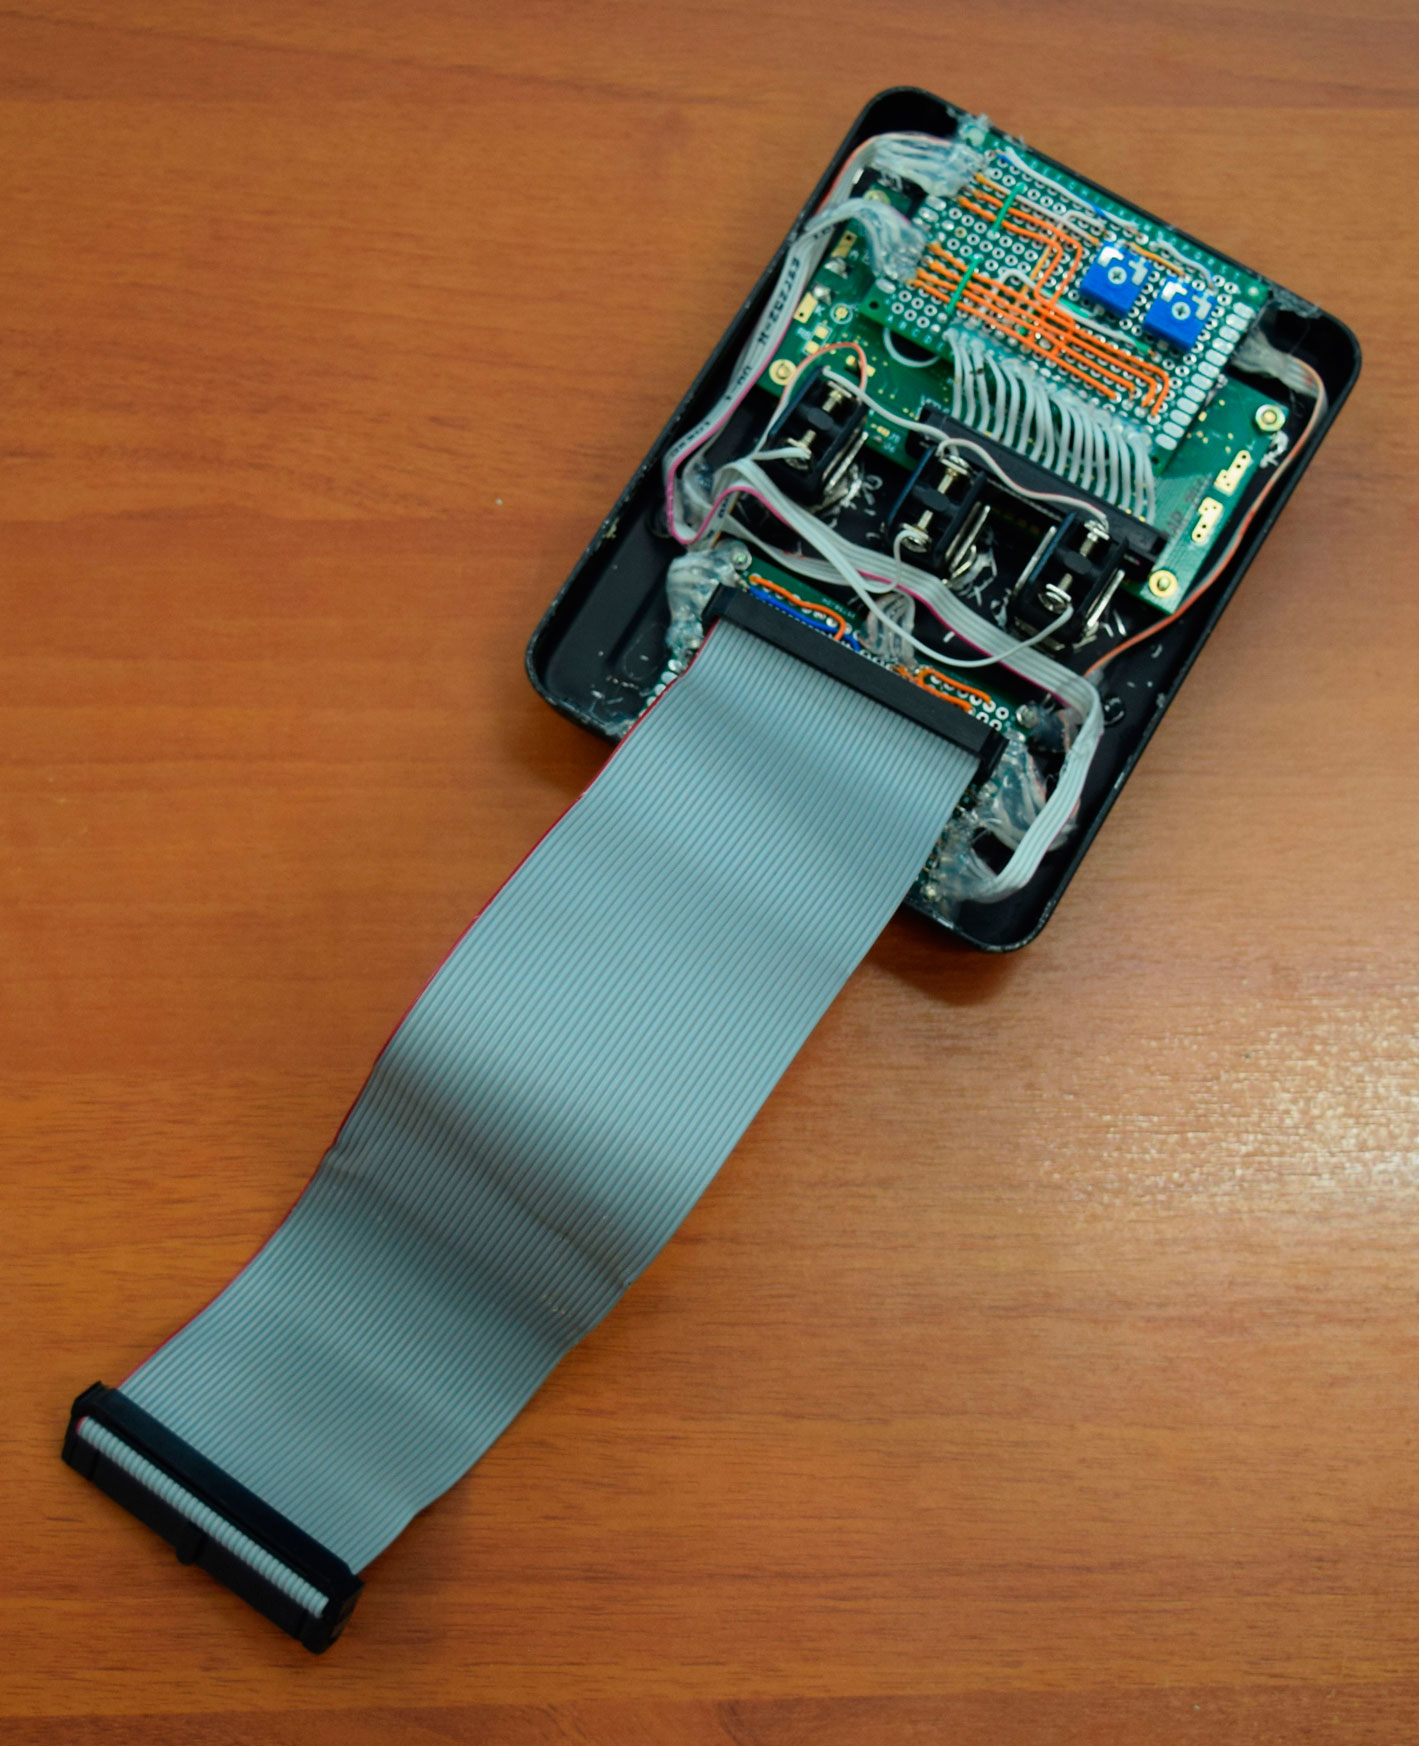
\includegraphics[width=0.7\textwidth]{img/prot-interno.jpg}
		\legend{Fonte: elaborado pelo autor}
	\end{minipage}
	\hfill
	\begin{minipage}{0.55\textwidth}
		\centering
		\caption{\label{fig:proto-teste}Protoboard na etapa de estudo}
		\includegraphics[width=1\textwidth]{img/proto-teste.jpg}
		\legend{Fonte: elaborado pelo autor}
	\end{minipage}
\end{figure}

Durante a fase de estudo das tecnologias utilizou-se uma protoboard e fios de conexão (\autoref{fig:proto-teste}) para testes de código, modo de conexão, entre outros, detalhado na \autoref{sec:segunda-etapa}.

Como o \textit{RPi} tem limitações quanto a quantidade de pinos de entrada e saída digitais (explicados na \autoref{sec:rpi-tecnologia}), os componentes definidos para o protótipo foram determinados conforme possibilidade de conexões. Cada componente necessita de:

\begin{alineas}
	\item um pino de saída digital (GPIO) para acender ou apagar cada LED;
	\item um pino de entrada digital para leitura do estado de cada botão;
	\item seis pinos de saída no total, sendo quatro de dados, um \textit{enable} (ou ativar), e outro \textit{register select}, para o display LCD.
\end{alineas}

O uso desses componentes foram determinados na segunda etapa, detalhada na \autoref{sec:segunda-etapa} - \nameref{sec:segunda-etapa}.


% ----------------------------------------------------------
\section{Tecnologias e Ferramentas}\label{sec:tecnologias-ferramentas}
% ----------------------------------------------------------


% ---
\subsection{Raspberry Pi}\label{sec:rpi-tecnologia}
% ---

O \textit{RPi} é a tecnologia mais importante desse projeto. Já foi abordado na \autoref{sec:raspberry-pi} e \autoref{sec:rpi-acessorios}, porém nessa seção outros aspectos serão comentados.

% TODO Falar das GPIOs, quantidade de pinos digitais, voltagem 3.3V


% ---
\subsection{Node.js e npm}\label{sec:node-js}
% ---

Node.js é uma plataforma de aplicações baseada no motor de Javascript do Google Chrome chamado V8. \cite{o-que-e-node}. A linguagem Javascript normalmente é utilizada no navegador, no chamado lado do cliente, porém o Node leva essa linguagem de programação diretamente para o sistema operacional, permitindo que aplicações sejam executadas direto no lado servidor. 

Utiliza um modelo de aplicações voltado a eventos, ou seja, não bloqueia a execução do código com entrada e saída, cálculos, etc. Em vez disso dispara as funções quando os eventos forem acionados. \cite{o-que-e-node}.

Essa plataforma possui um aplicativo chamado \textit{Node Package Manager} (denominado \textit{npm}).

% TODO falar dos pacotes utilizados, npm

% ---
\subsection{CouchDB}\label{sec:couchdb}
% ---



% ---
\subsection{Git}\label{sec:git}
% ---

Git é um software de controle de versão para repositórios. Registra as mudanças nos arquivos (ou grupo de arquivos) ao longo do tempo, de forma que as versões possam ser recuperadas futuramente. \cite{pro-git}. Caso necessário voltar algumas versões por \textit{bug} no código, mal funcionamento de uma função recém implementada ou outras razões, as alterações estarão todas salvas.

Atualmente o Git é muito utilizado por projetos de código aberto, como por exemplo o Swift\footnote{\url{https://github.com/apple/swift}} que é uma linguagem de programação criada pela Apple voltada para seus sistemas operacionais, e o AngularJS\footnote{\url{https://github.com/angular/angular.js}}, framework Javascript mantido pelo Google.

É possível configurar o repositório local para sincronizar com um repositório remoto, por meio de \textit{push} (enviar mudanças) e \textit{pull} (buscar mudanças). Dessa forma promove a divisão do trabalho, removendo o problema de sincronização de código entre diferentes máquinas e pessoas.

% ---
\subsubsection{GitHub}\label{sec:github}
% ---



% ---
\subsection{Outras Ferramentas}\label{sec:outras-ferramentas}
% ---

Durante o desenvolvimento desse trabalho foi necessário a criação de uma proposta e um relatório parcial, ambos para a disciplina de Projeto e Implementação de Sistemas I. Para tal, o autor utilizou a ferramenta denominada LaTeX. Como não está entre os objetivos desse projeto, mas houve um grande crescimento no seu uso, está detalhada no \autoref{ap:latex}.


% ----------------------------------------------------------


% ----------------------------------------------------------
% Experimentos e Resultados
% ----------------------------------------------------------
\chapter{Desenvolvimento}\label{cap:desenvolvimento}
% ----------------------------------------------------------

% ----------------------------------------------------------
\section{Primeira Etapa - Estudo Prático das Tecnologias}\label{sec:primeira-etapa}
% ----------------------------------------------------------

O primeiro experimento realizado foi a tentativa de identificação de um \textit{beacon} com o \textit{RPi}, para o estudo de funcionamento e comportamento dessas tecnologias. Para isso, o ambiente foi configurado conforme \autoref{fig:inicio-ambiente}. 

\begin{figure}[htb]
	\caption{\label{fig:inicio-ambiente}Primeiro teste realizado, com \textit{RPi} e \textit{beacon MPact}}
	\begin{center}
		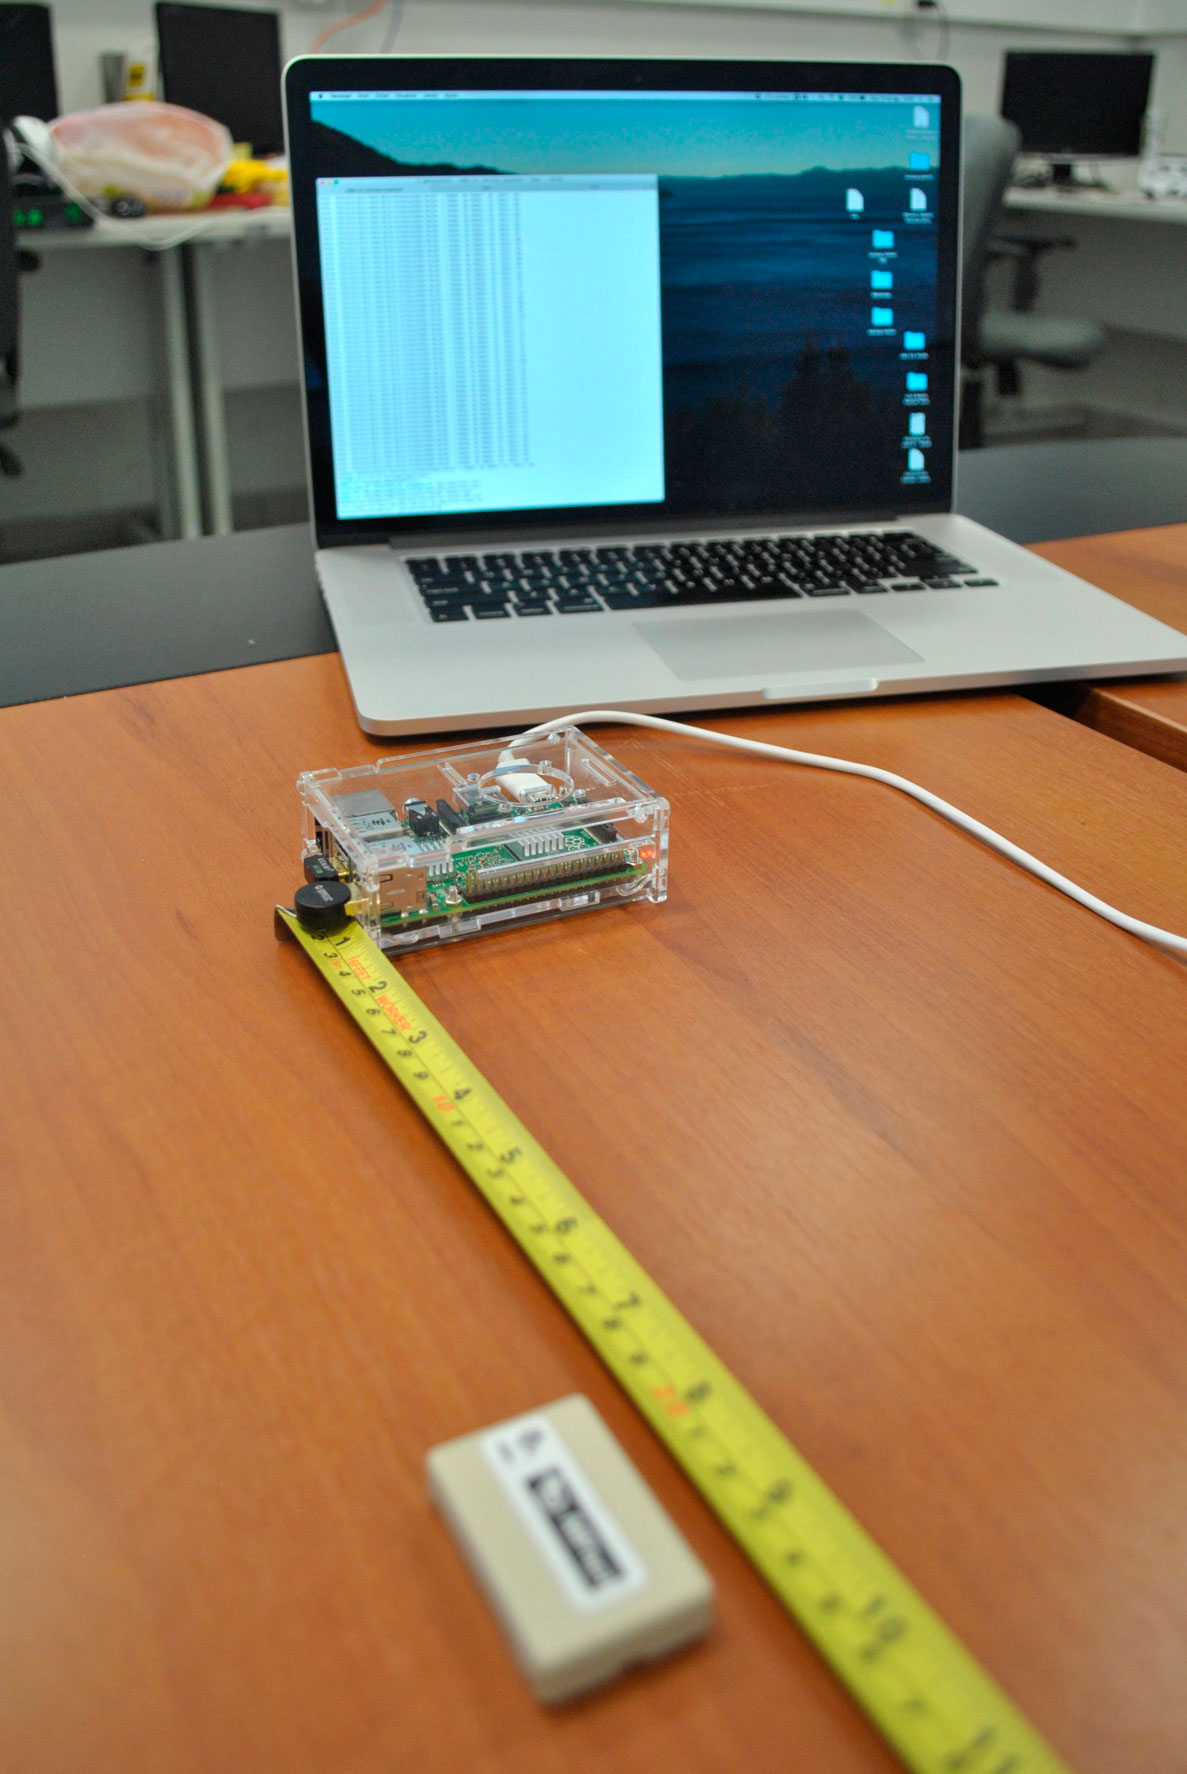
\includegraphics[width=0.66\textwidth]{img/ambiente1.jpg}
	\end{center}
	\legend{Fonte: elaborado pelo autor}
\end{figure}

O computador ficou conectado via SSH com o \textit{RPi}, recebendo as informações de leitura de pacotes \textit{BLE}. Os softwares utilizados para isso foram, conforme \citeonline{stack-overflow-ibeacon}, os seguintes:

\begin{alineas}
	\item \textbf{hcitool}: configurado da maneira \textit{hcitool lescan --duplicates}, faz um scan na frequência \textit{BLE} procurando por dispositivos que estejam transmitindo, conforme \autoref{fig:hcitool-lescan}.
	
	\begin{figure}[htb]
		\caption{\label{fig:hcitool-lescan}Software \textit{hcitool} executando}
		\begin{center}
			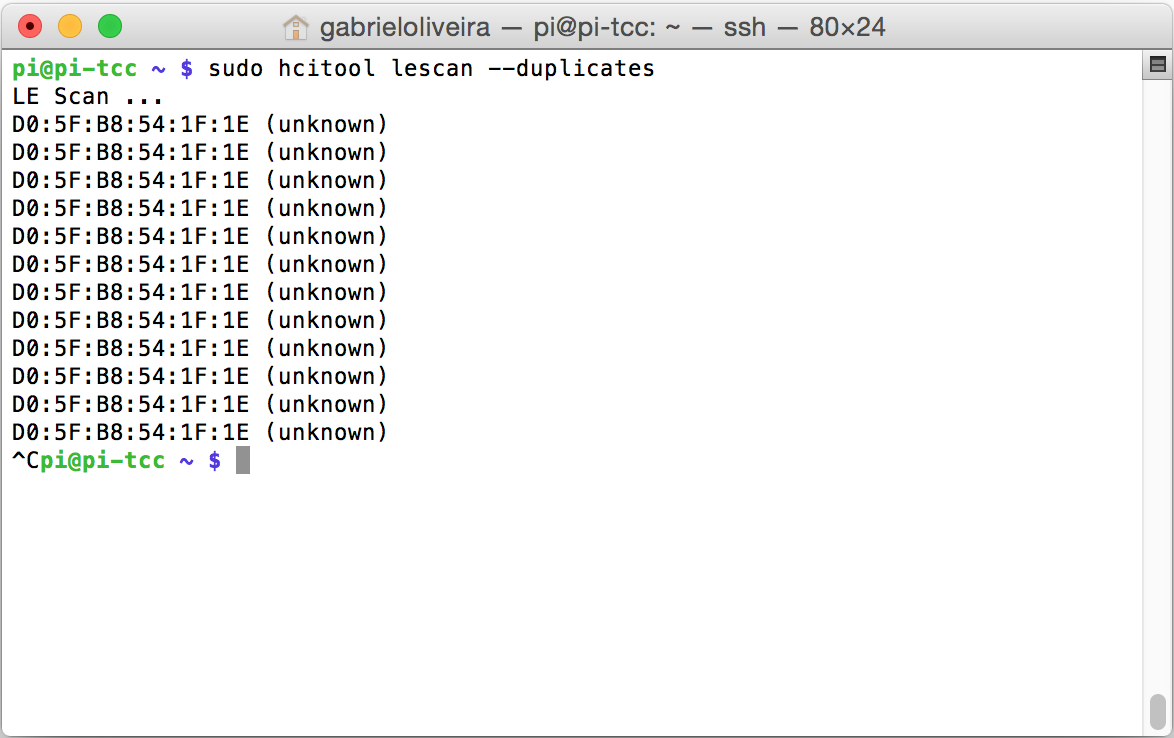
\includegraphics[width=0.6\textwidth]{img/hcitool-lescan.png}
		\end{center}
		\legend{Fonte: elaborado pelo autor}
	\end{figure}

	\item \textbf{hcidump}: em conjunto com o \textit{hcitool}, apresenta todos os pacotes escaneados na rede. Executado da maneira \textit{hcidump --raw}, conforme \autoref{fig:hcidump}.
	
	\begin{figure}[htb]
		\caption{\label{fig:hcidump}Software \textit{hcidump} executando}
		\begin{center}
			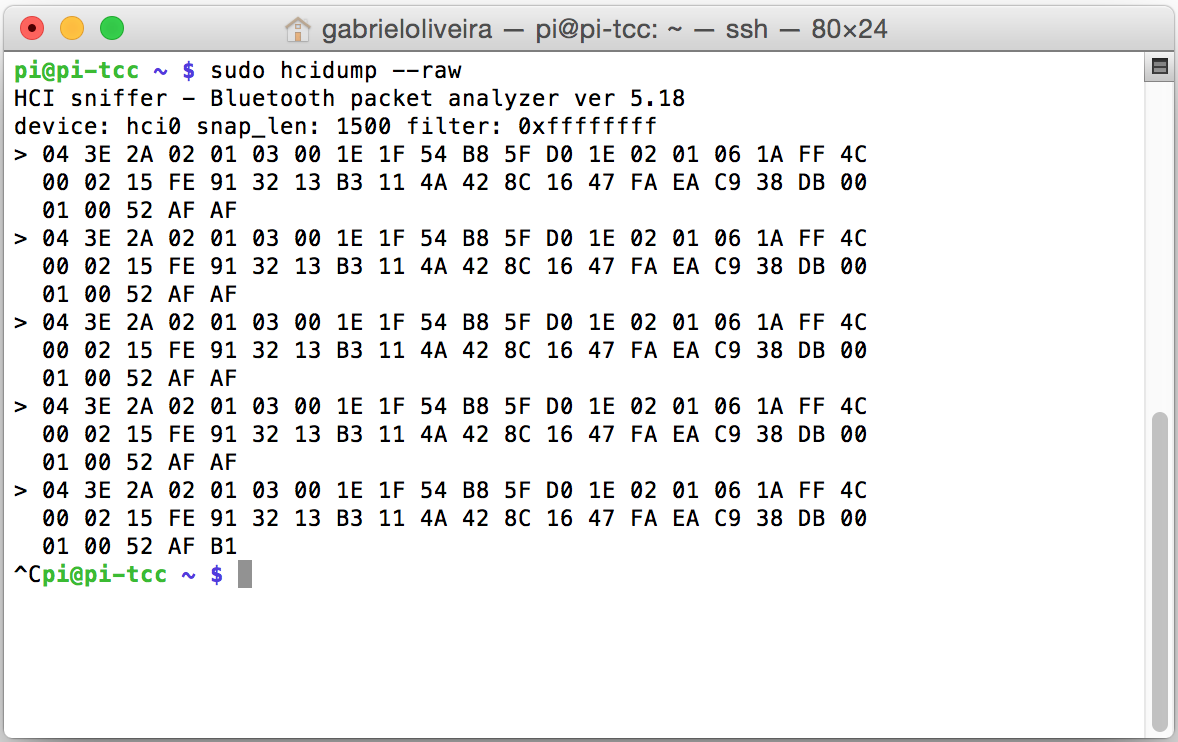
\includegraphics[width=0.6\textwidth]{img/hcidump.png}
		\end{center}
		\legend{Fonte: elaborado pelo autor}
	\end{figure}

\end{alineas}

Em seguida, com os softwares em execução e os pacotes sendo analisados, o \textit{beacon} foi movido ao longo mesa para ficar a diferentes distâncias do \textit{RPi}, conforme \autoref{fig:movimenta-beacon}. Esse passo foi necessário para verificar o formato dos pacotes recebidos e também analisar a distância máxima de identificação.

\begin{figure}[htb]
	\caption{\label{fig:movimenta-beacon}Teste com movimentação do \textit{beacon}}
	\begin{center}
		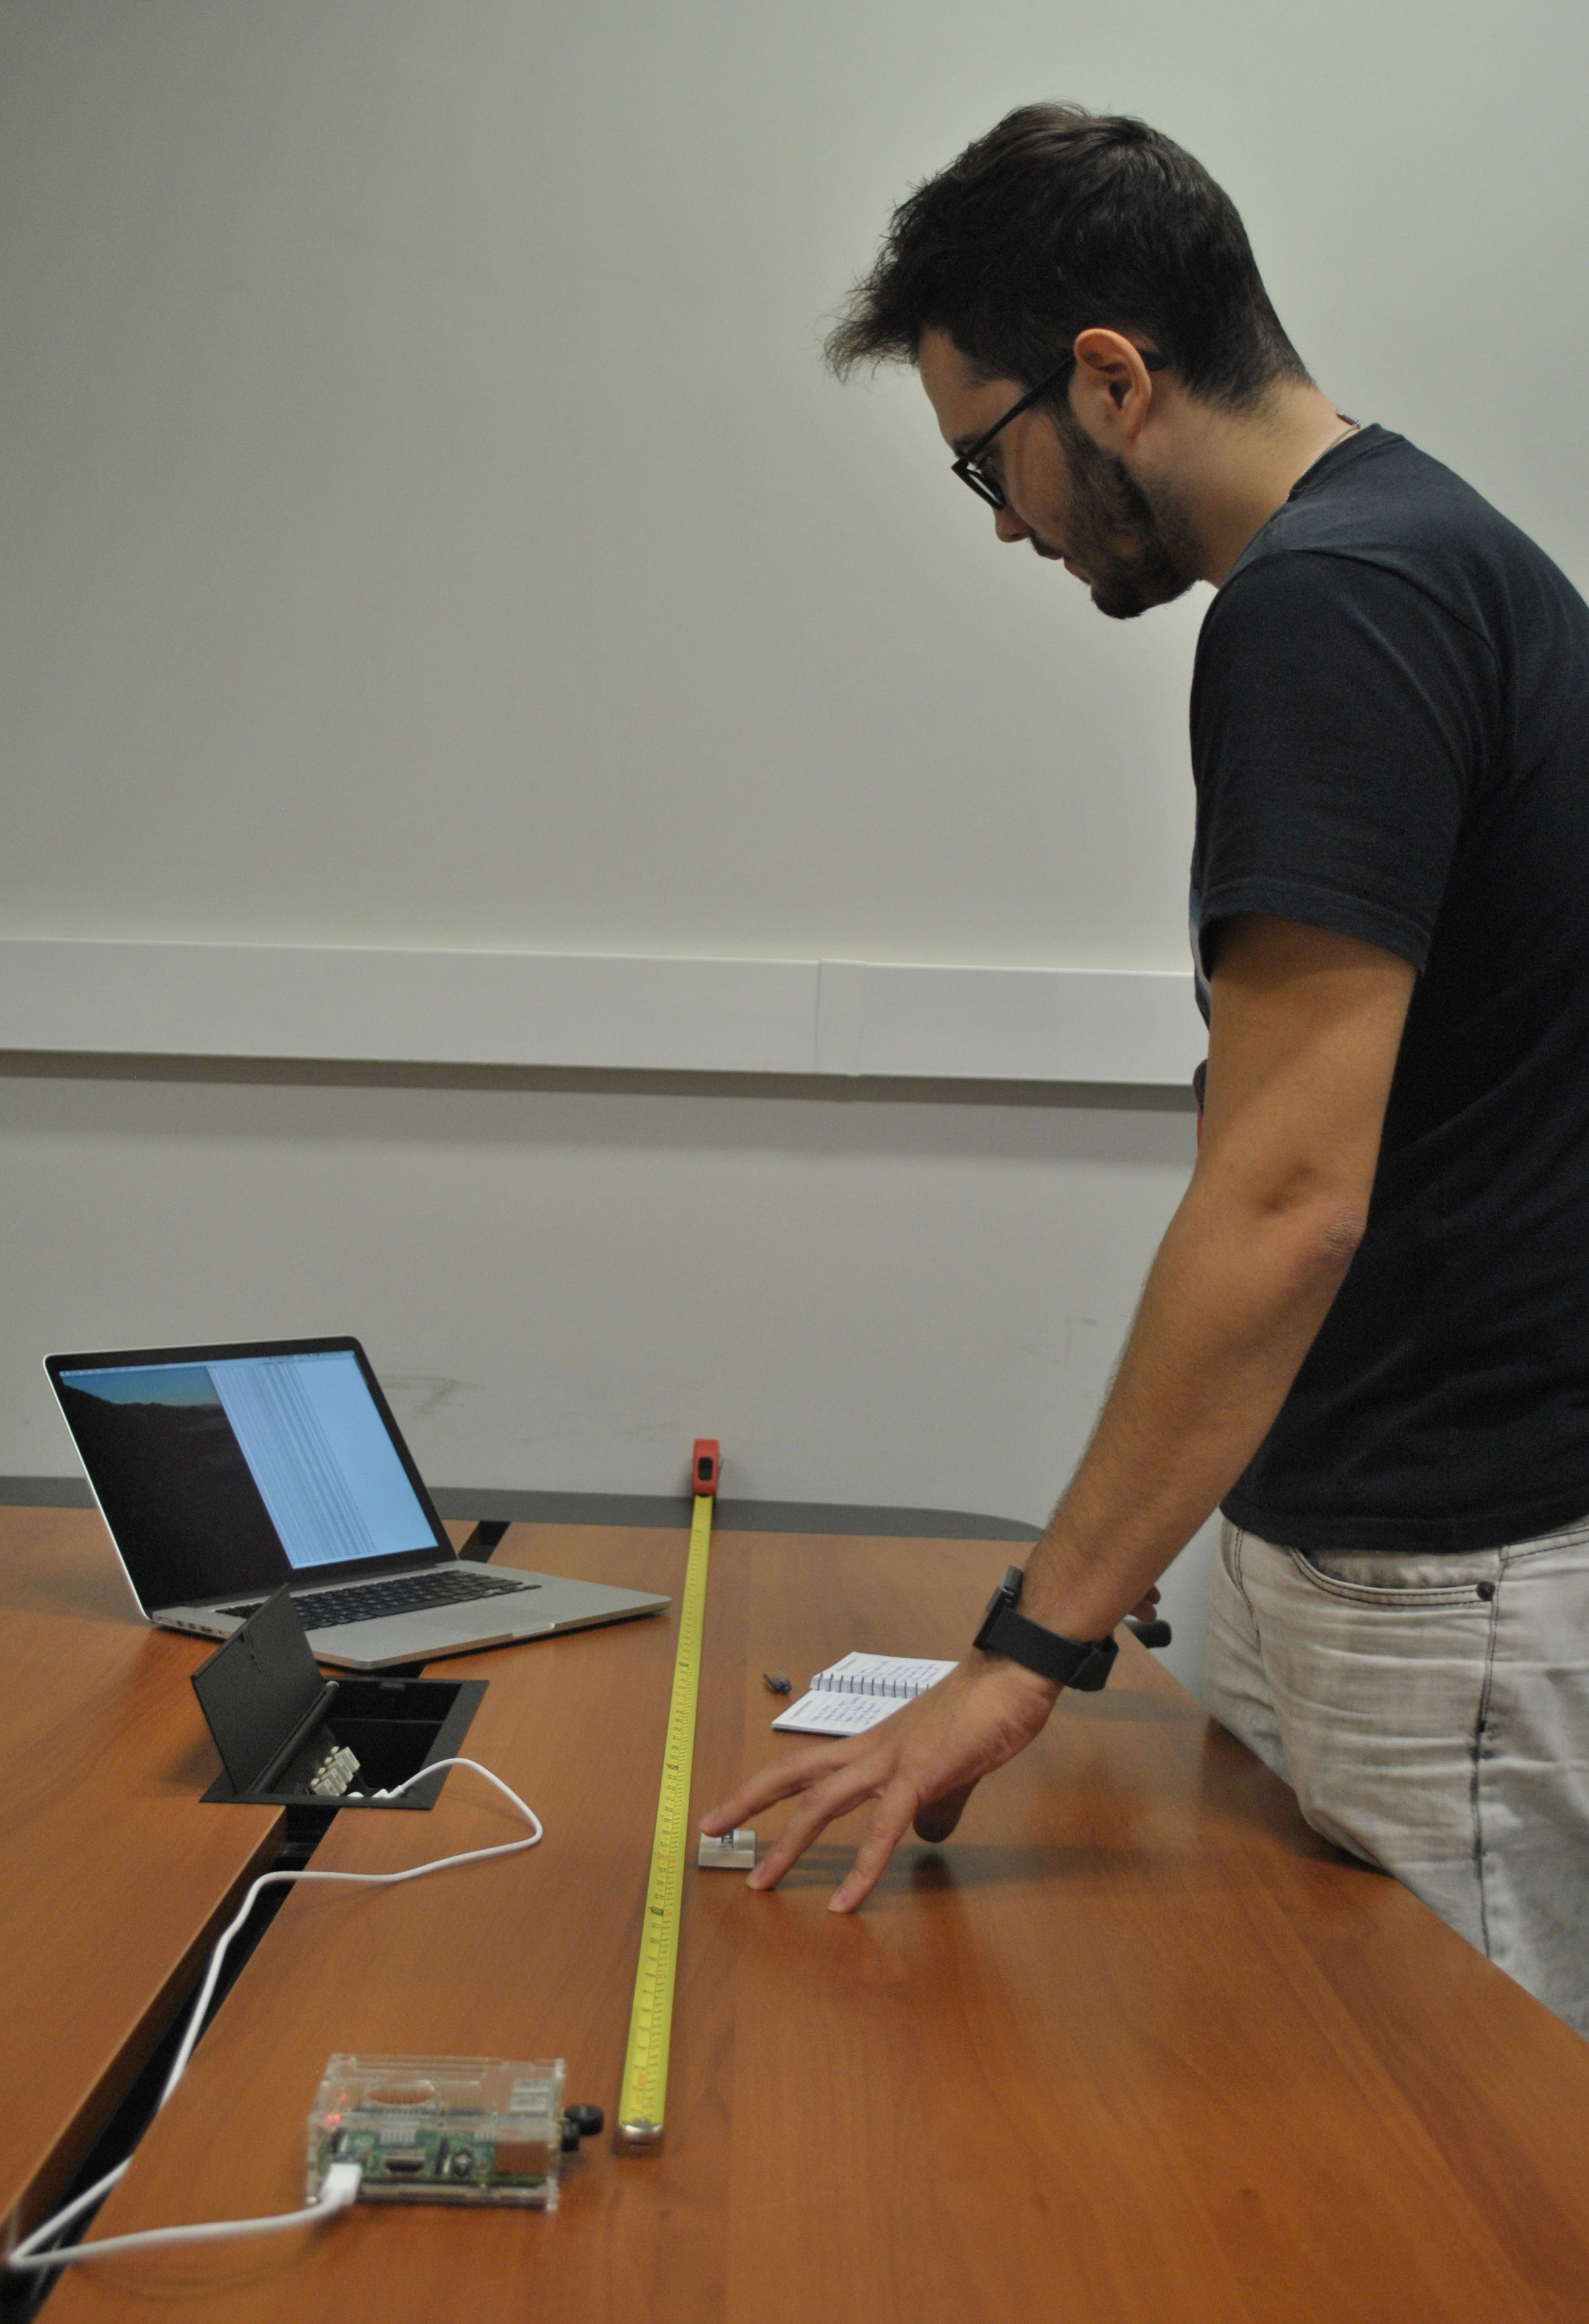
\includegraphics[width=0.7\textwidth]{img/ambiente4.jpg}
	\end{center}
	\legend{Fonte: elaborado pelo autor}
\end{figure}

Com o adaptador Orico BTA-406 e posicionamento na mesa conforme \autoref{fig:inicio-ambiente} e \autoref{fig:movimenta-beacon}, a cerca de 1,3 a 1,4 metros de distância entre o \textit{RPi} e o \textit{beacon} os pacotes já começaram a falhar e a leitura não foram tão constante.

O posicionamento do \textit{RPi} foi alterado para testes, conforme \autoref{fig:posiciona-rpi}. Notou-se uma melhoria na recepção dos pacotes, a 1,5 metros entre o \textit{RPi} e o \textit{beacon} os pacotes começaram a falhar, com recebimento de informações notada até 1,6 metros.

\begin{figure}[htb]
	\caption{\label{fig:posiciona-rpi}\textit{RPi} posicionado de outra maneira}
	\begin{center}
		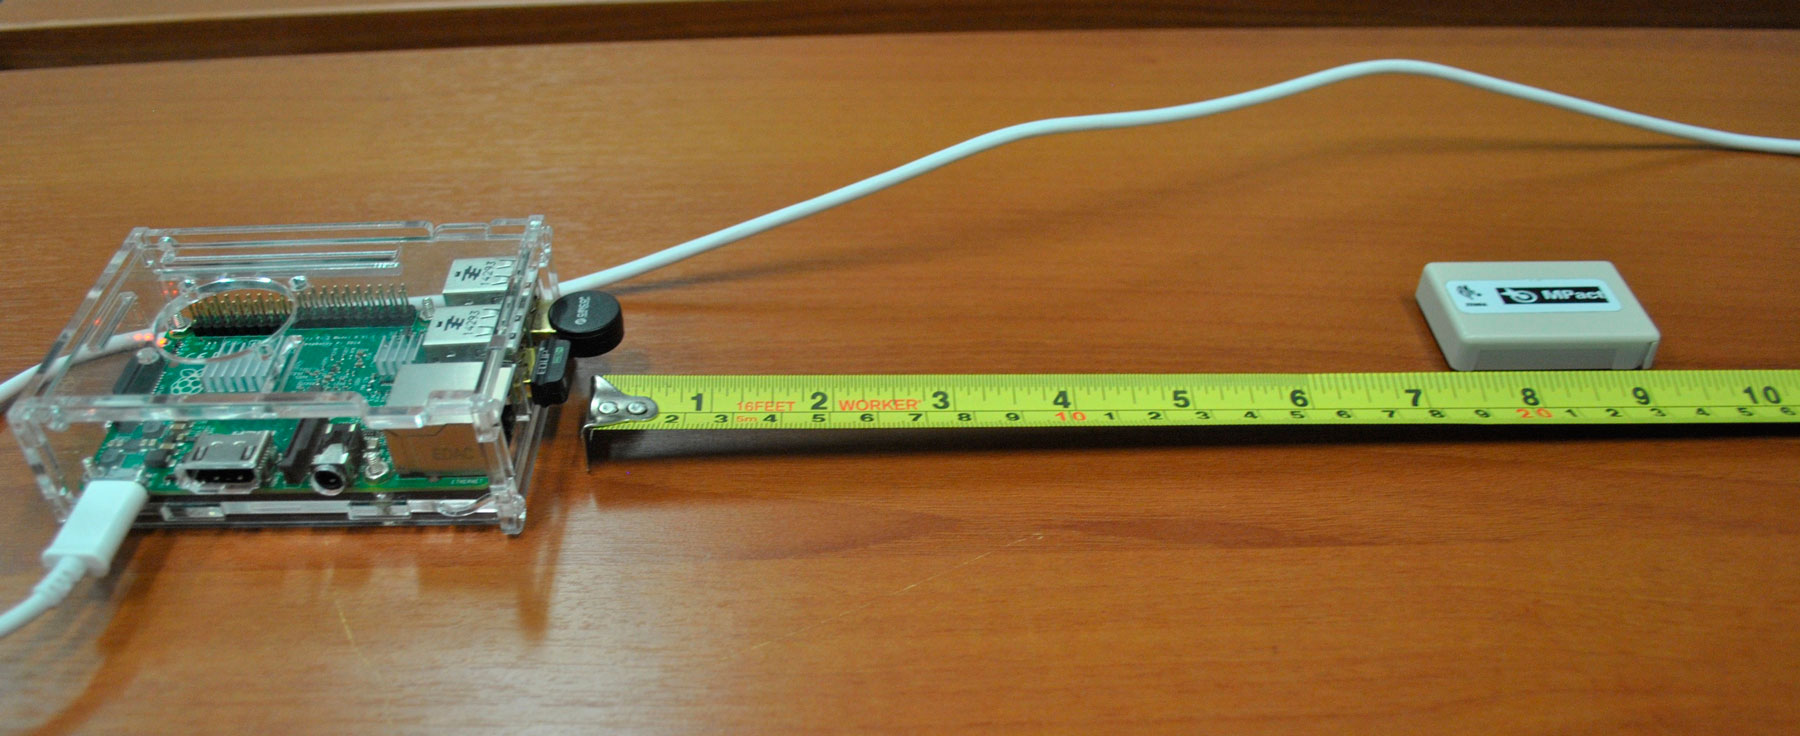
\includegraphics[width=0.8\textwidth]{img/ambiente2.jpg}
	\end{center}
	\legend{Fonte: elaborado pelo autor}
\end{figure}

Durante essa etapa não foram levados em consideração conexões com LEDs, botões e display LCD para a montagem do protótipo pois esses componentes foram definidos posteriormente. Os estudos e testes desses materiais foram realizados na segunda etapa, para que as escolhas fossem validadas.

% ----------------------------------------------------------
\section{Segunda Etapa - Planejamento do Protótipo}\label{sec:segunda-etapa}
% ----------------------------------------------------------

Para que o protótipo pudesse ser bem planejado, parâmetros foram definidos:

\begin{alineas}
	\item ter uma interface amigável e simples para interação com o software;
	\item ser bem apresentável, com cores marcantes e boa construção;
	\item mostrar informações relevantes sobre o sistema - aplicação, software e sistema (Linux e \textit{RPi});
	\item ser construído em um único pacote, não muito grande nem muito pequeno;
\end{alineas}

Seguindo esses parâmetros, a primeira busca foi por um recipiente para alocar todos os componentes necessários, de forma que tudo ficasse bem protegido. Para tal, escolheu-se uma caixa de metal, derivada de uma antiga caixa de cigarros, apresentado na \autoref{sec:acess-prototipo}.

O material foi cortado primeiramente na parte de baixo de forma que acomodasse o \textit{RPi} deixando todas as conexões disponíveis para futuro desenvolvimento e facilidade de acessar as portas. Foram realizados furos na parte do fundo para fixação do \textit{RPi} com parafusos, arruelas e porcas, conforme \autoref{fig:rpi-caixa}.

% TODO - FOTO DO FUNDO COM OS PARAFUSOS

\begin{figure}[htb]
	\caption{\label{fig:rpi-caixa}\textit{RPi} preso na caixa, com as portas acessíveis}
	\begin{center}
		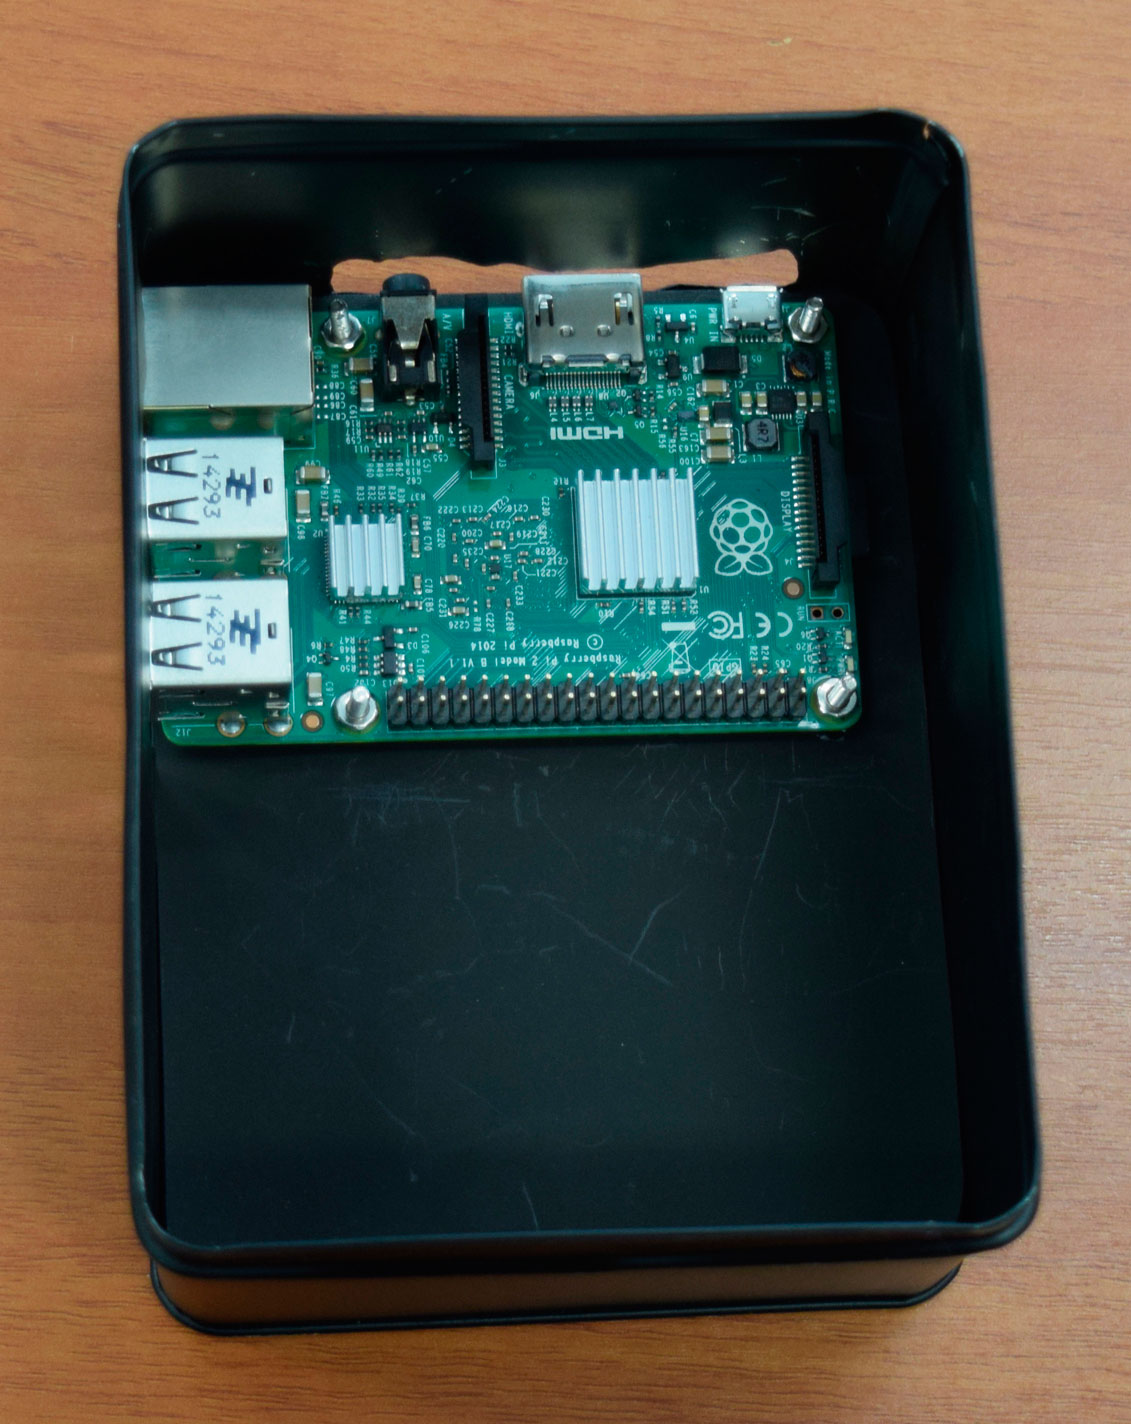
\includegraphics[width=0.6\textwidth]{img/rpi-caixa.jpg}
	\end{center}
	\legend{Fonte: elaborado pelo autor}
\end{figure}

Dessa maneira o RPi ficou bem preso na parte de baixo, liberando a tampa para instalação da interface com o usuário.

O próximo passo foi para definir a interface com o usuário. Para que os parâmetros fossem cumpridos, os seguintes itens necessários foram elencados:

\begin{alineas}
	\item apresentar informação em que consistia se o sistema está rodando a aplicação corretamente - para tal definiu-se o uso de um LED verde;
	\item apresentar informação em que consistia se o sistema tem conexão com a internet - para tal definiu-se o uso de um LED amarelo;
	\item apresentar informação em que consistia se um beacon está no alcance - para tal definiu-se o uso de um LED azul;
	\item apresentar várias informações textuais sobre o estado atual do sistema, assim como beacons no alcance, histórico, dados do Linux, endereço de IP, temperatura da CPU - para tal, definiu-se o uso de um display LCD de 16 colunas por 2 linhas.
\end{alineas}

Como o display era pequeno e não apresentou todas as informações de uma só vez, decidiu-se pela utilização de navegação por páginas, de forma que as informações fossem alteradas conforme avançasse nas páginas. Para que a navegação fosse realizada de maneira agradável e apresentável, os seguintes itens foram escolhidos:

\begin{alineas}
	\item LEDs indicando qual página está - definiu-se pelo uso de três LEDs verde;
	\item botões do tipo clique para navegar a direita e esquerda nas páginas principais, e entre as páginas secundárias.
\end{alineas}

Com os componentes bem definidos, a interface foi concebida inicialmente em rascunhos no papel. Foi necessário realizar testes com os LEDs, display LCD e botões na protoboard de forma que todos esses componentes pudessem ser conectados ao mesmo tempo (\autoref{fig:proto-lcd} e \autoref{fig:proto-leds}). 

\begin{figure}[htb]
	\centering
 	\begin{minipage}{0.47\textwidth}
		\centering
		\caption{\label{fig:proto-lcd}Estudo de conexão e programação com display LCD}
		\includegraphics[width=1\textwidth]{img/proto-lcd.jpg}
		\legend{Fonte: elaborado pelo autor}
	\end{minipage}
	\hfill
	\begin{minipage}{0.47\textwidth}
		\centering
		\caption{\label{fig:proto-leds}Conexão com LEDs, display e botão na protoboard}
		\includegraphics[width=1\textwidth]{img/proto-leds.jpg}
		\legend{Fonte: elaborado pelo autor}
	\end{minipage}
\end{figure}

Nesse momento definiu-se o uso de Node.js (detalhado na \autoref{sec:node-js}) para o desenvolvimento, pois foram encontrados diversos tutoriais\footnote{\url{http://thejackalofjavascript.com/rpi-16x2-lcd-print-stuff/}}\footnote{\url{http://odesenvolvedor.andafter.org/publicacoes/controlando-gpio-do-raspberrypi-com-nodejs.html}}\footnote{\url{https://learn.adafruit.com/node-embedded-development/why-node-dot-js}} e bibliotecas\footnote{\url{https://www.npmjs.com/package/lcd}}\footnote{\url{https://www.npmjs.com/package/onoff}} que facilitaram a conexão com todos os componentes.

Após realizar todos os estudos e testes de conexão com sucesso, o próximo passo foi a montagem da interface na caixa de metal. Primeiro os cortes foram feitos com uma ferramenta específica tipo esmeril, em seguida a caixa foi pintada com tinta preta fosca (\autoref{fig:pintar-1} e \autoref{fig:pintar-2}) para que o protótipo ficasse com boa construção e visualização.

Foram necessários soldas e montagem dos outros componentes em placas para que tudo ficasse organizado e fácil de ser trocado, caso necessário. As conexões das GPIOs com os componentes de hardware estão marcados na \autoref{fig:pinout-gpio}.

\begin{figure}[htb]
	\centering
 	\begin{minipage}{0.45\textwidth}
		\centering
		\caption{\label{fig:pintar-1}Pintura da caixa de metal - tampa}
		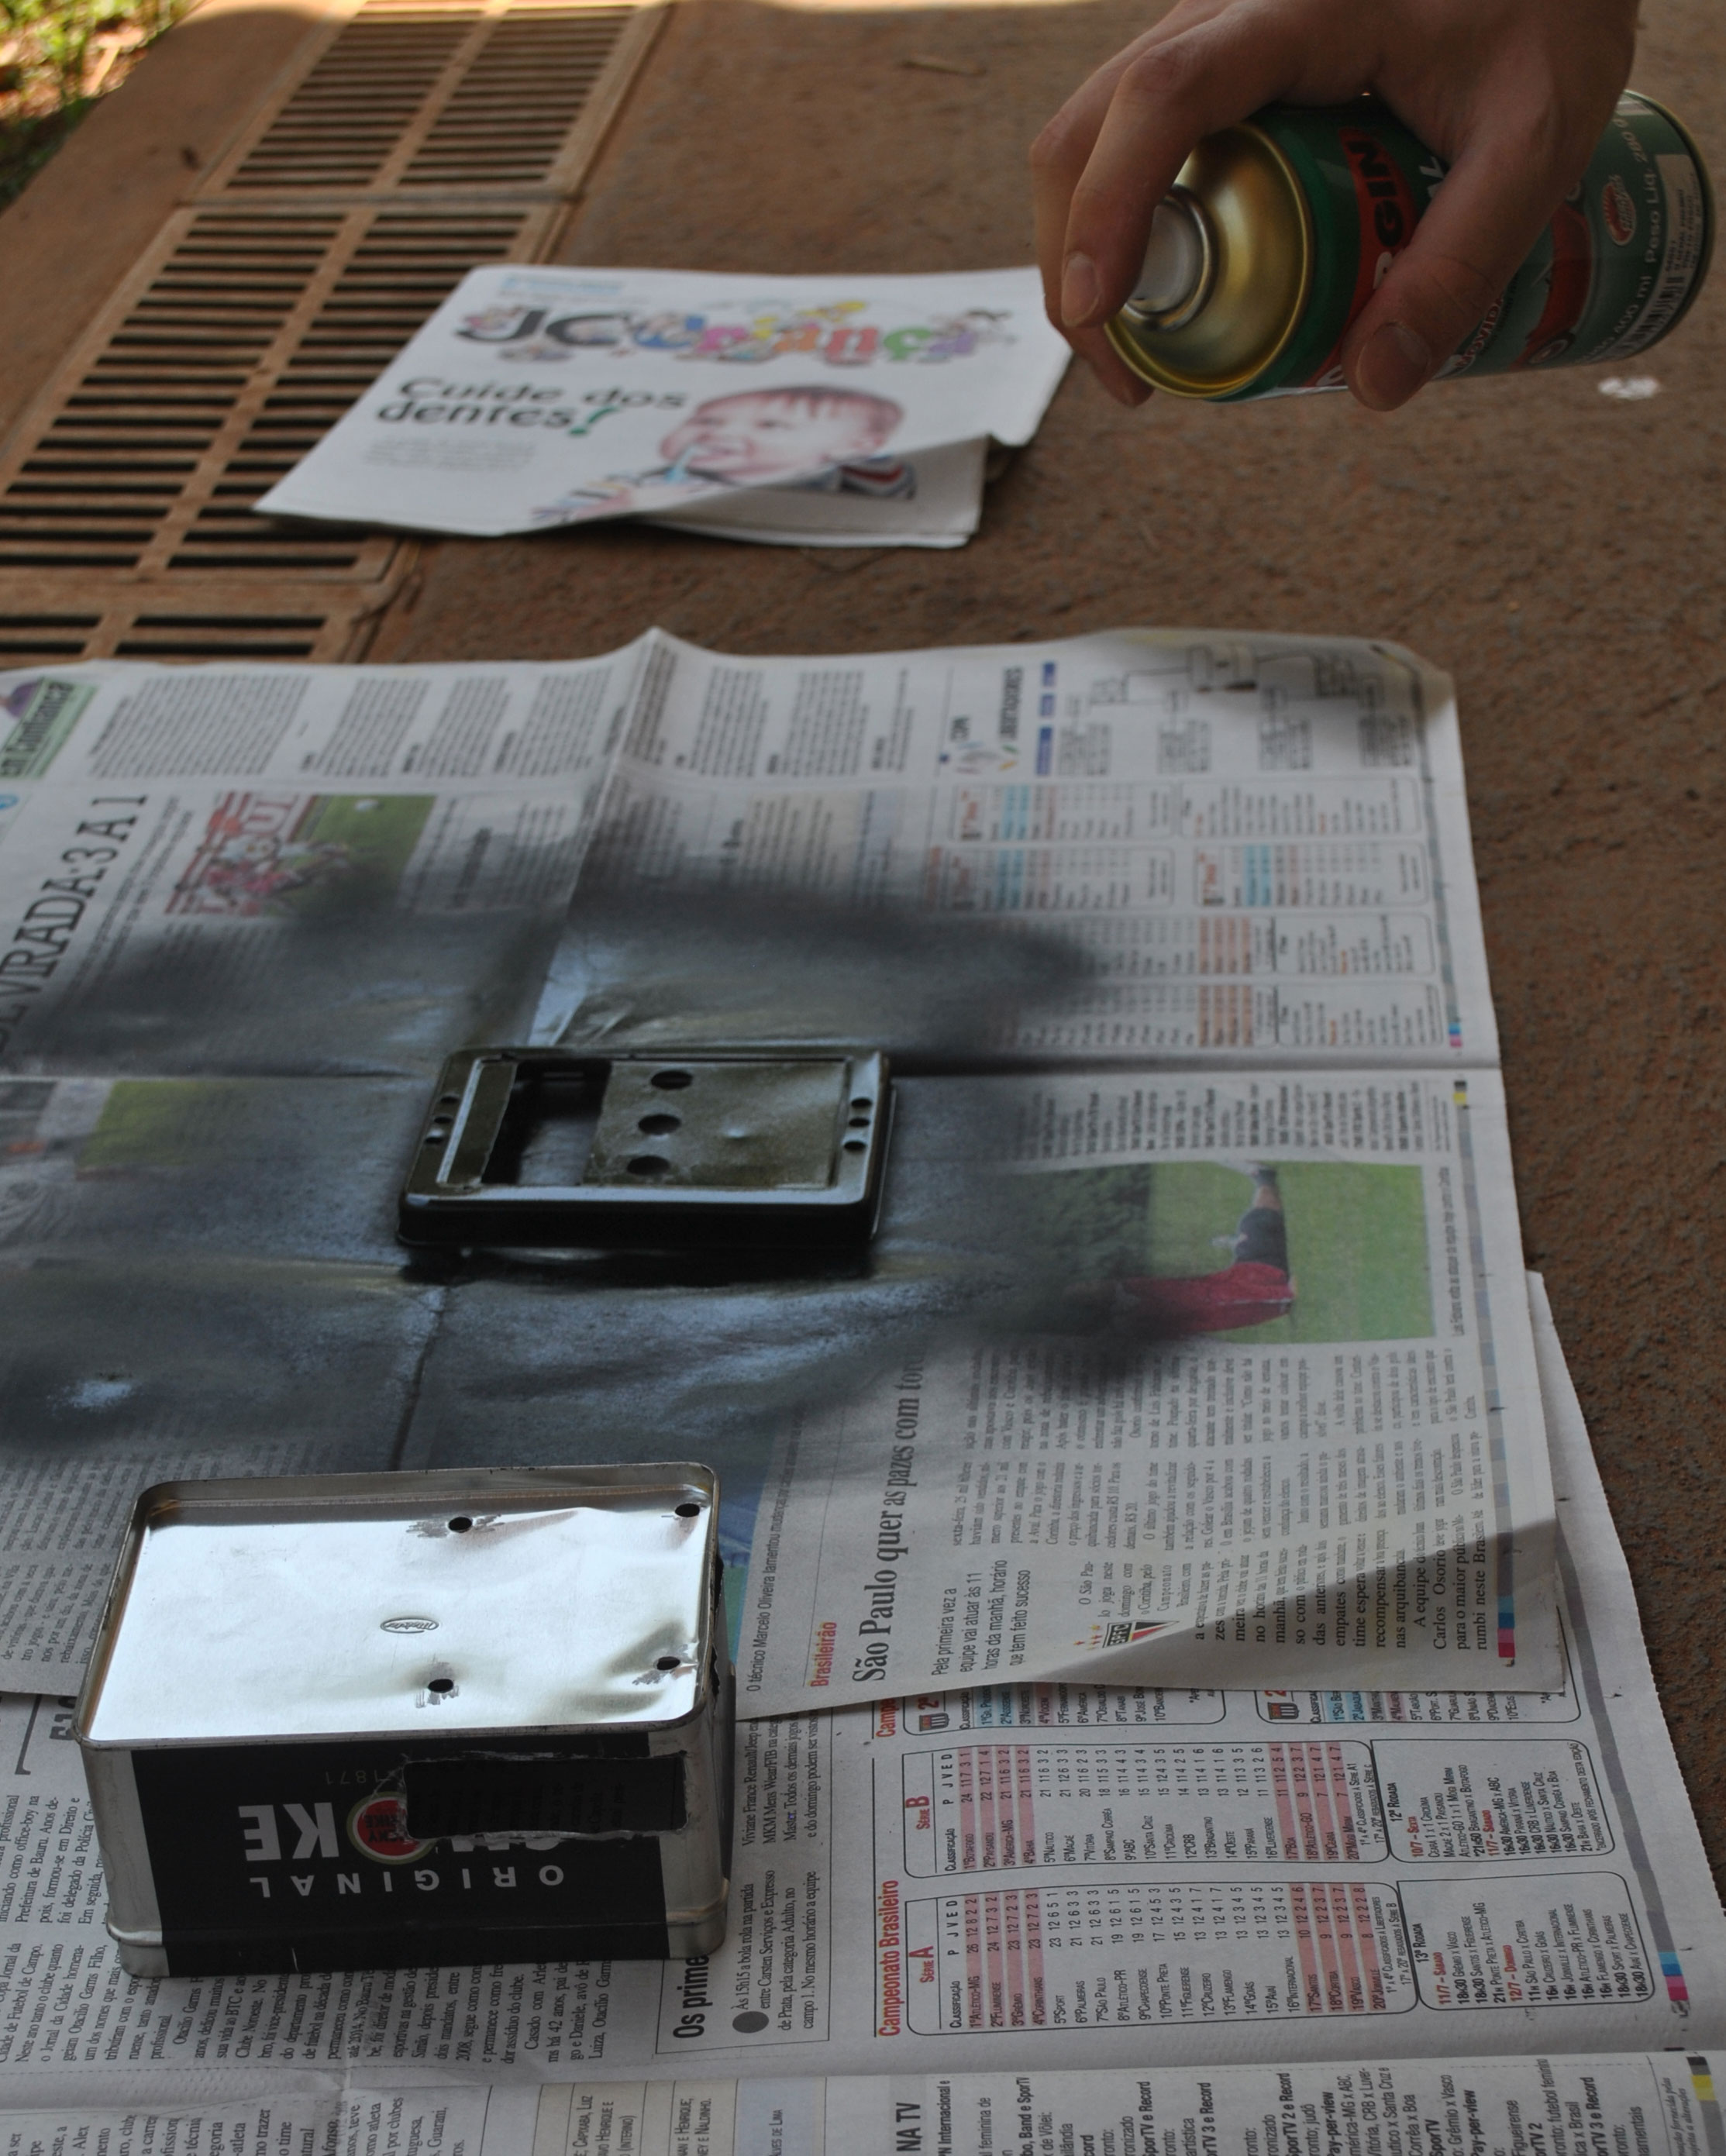
\includegraphics[width=1\textwidth]{img/pintar-1.jpg}
		\legend{Fonte: elaborado pelo autor}
	\end{minipage}
	\hfill
	\begin{minipage}{0.45\textwidth}
		\centering
		\caption{\label{fig:pintar-2}Pintura da caixa de metal - base}
		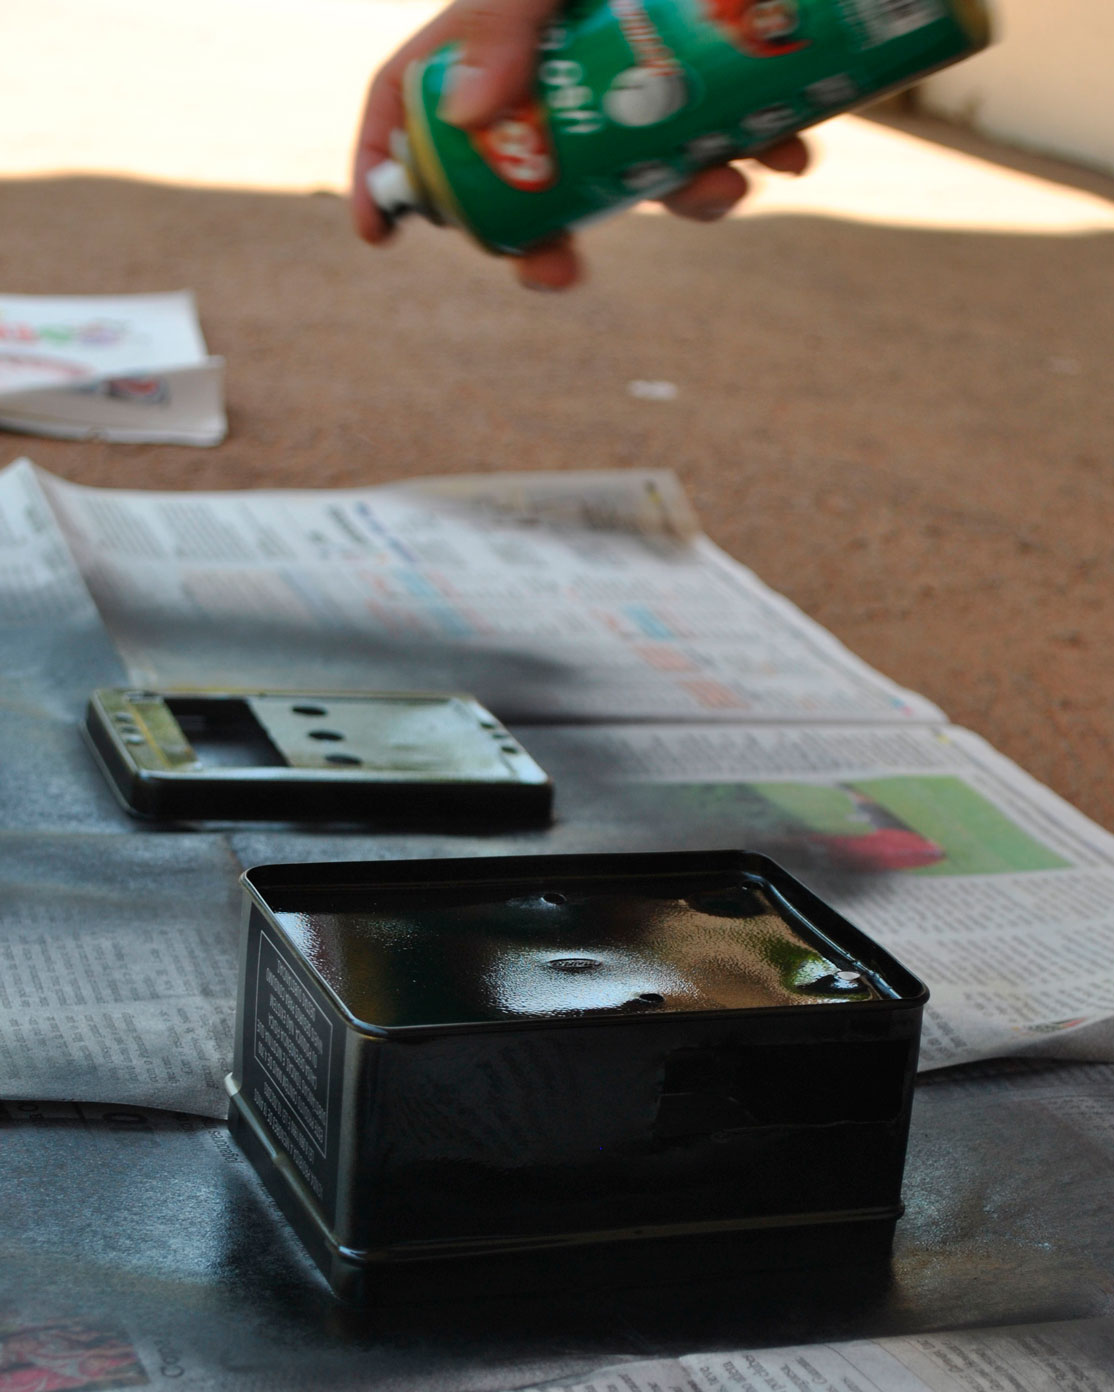
\includegraphics[width=1\textwidth]{img/pintar-2.jpg}
		\legend{Fonte: elaborado pelo autor}
	\end{minipage}
\end{figure}

Cada LED foi conectado a uma GPIO, a um resistor de 330$\Omega$, e ao GND. Os botões foram conectados seguindo o modelo da \autoref{fig:push-btn-sketch}. O display foi conectado diretamente a cada GPIO marcada, e também ao +5V e GND para alimentação. 

O modelo de display LCD utilizado também tem um pino que utiliza voltagem variável para iluminar cada caractere (contraste de cada letra), e um pino para a iluminação do fundo (azul). Para essas conexões foram utilizados potenciômetros de 10K, para facilitar mudanças caso necessário (\autoref{fig:potentiometer}). Dessa forma, só é necessário girar o pino do potenciômetro para alterar a saída.

\begin{figure}[htb]
	\centering
 	\begin{minipage}{0.45\textwidth}
		\centering
		\caption{\label{fig:push-btn-sketch}Modelo de conexão dos botões}
		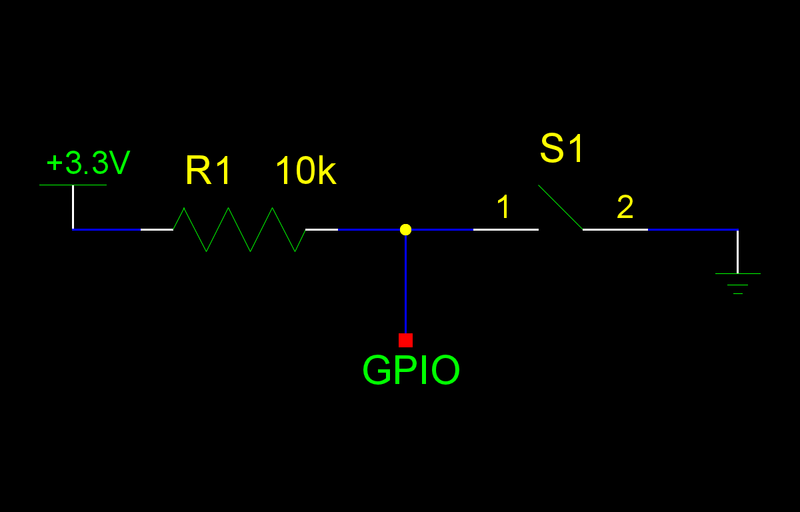
\includegraphics[width=1\textwidth]{img/push-btn-sketch.png}
		\legend{Fonte: \cite{push-button}}
	\end{minipage}
	\hfill
	\begin{minipage}{0.45\textwidth}
		\centering
		\caption{\label{fig:potentiometer}Potenciômetros de configuração do display LCD}
		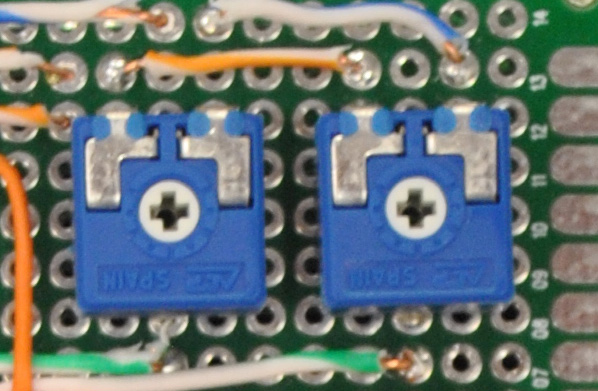
\includegraphics[width=1\textwidth]{img/potentiometer.jpg}
		\legend{Fonte: elaborado pelo autor}
	\end{minipage}
\end{figure}

\begin{figure}[htb]
	\caption{\label{fig:pinout-gpio}Circuito de conexão das GPIOs}
	\begin{center}
		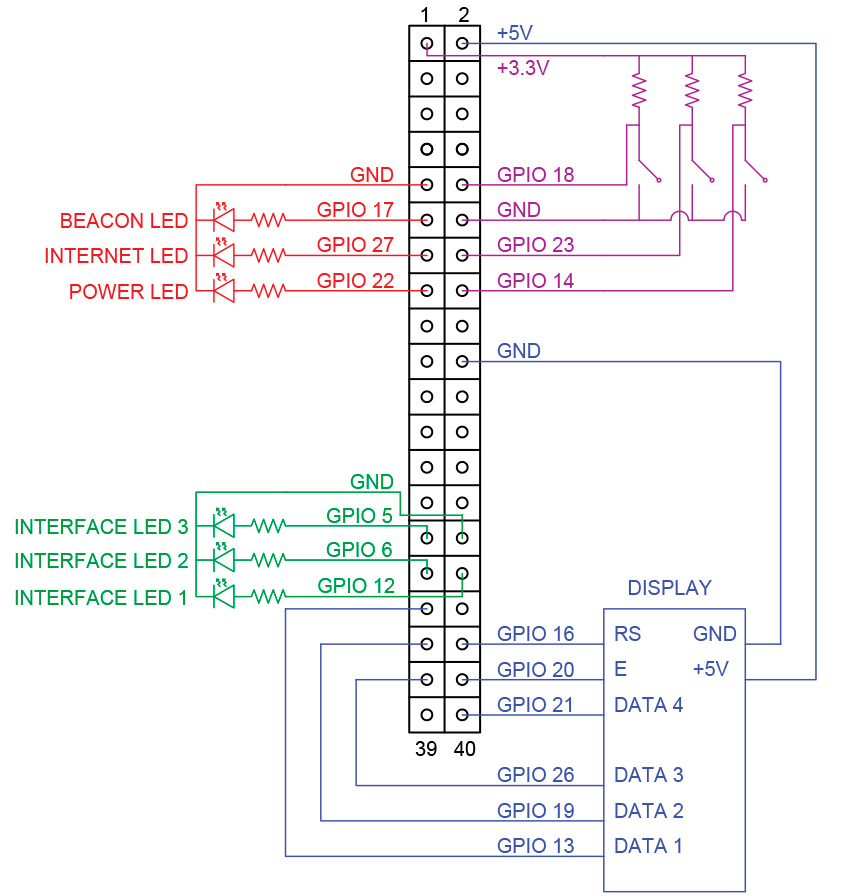
\includegraphics[width=0.8\textwidth]{img/pinout-gpio.jpg}
	\end{center}
	\legend{Fonte: elaborado pelo autor}
\end{figure}


Foram utilizados seis GPIOs para os LEDs, três para os botões e seis para o display, totalizando 15 GPIOs de 17 disponíveis. As GPIOs utilizadas foram:

\begin{alineas}
	\item Para os LEDs de interface (topo), GPIO 12, 6 e 5, respectivamente 1, 2 e 3;
	\item Para os LEDs de informação (baixo), GPIO 22, 27 e 17, respectivamente Power, Internet e Beacon;
	\item Para os botões, GPIOs 24, 23 e 18, respectivamente botão esquerdo, central e direito;
	\item Para o display de LCD, GPIOs 16, 20, 13, 19, 26, 21, respectivamente Register Select, Enable, Data 1, Data 2, Data 3 e Data 4.
	\nota{Os números das GPIOs foram escolhidos devido a proximidade e agrupamento dos componentes.}
\end{alineas}

De forma que a tampa saísse facilmente optou-se por usar um cabo flat frequentemente usado em HDs antigos (padrão IDE) conectado ao \textit{RPi} e a uma placa central com duas fileiras de 20 pinos.

Utilizando os fios internos de cabo de rede para conexão entre os componentes nas placas, o mesmo cabo flat cortado para conexão entre as placas para uma maior flexibilidade e facilidade de mudanças, criou-se o controle da interface, como pode ser visto na \autoref{fig:interface-traz1} e \autoref{fig:interface-traz2}.

\begin{figure}[htb]
	\centering
 	\begin{minipage}{0.45\textwidth}
		\centering
		\caption{\label{fig:interface-traz1}Parte interna da interface - parcialmente desmontada}
		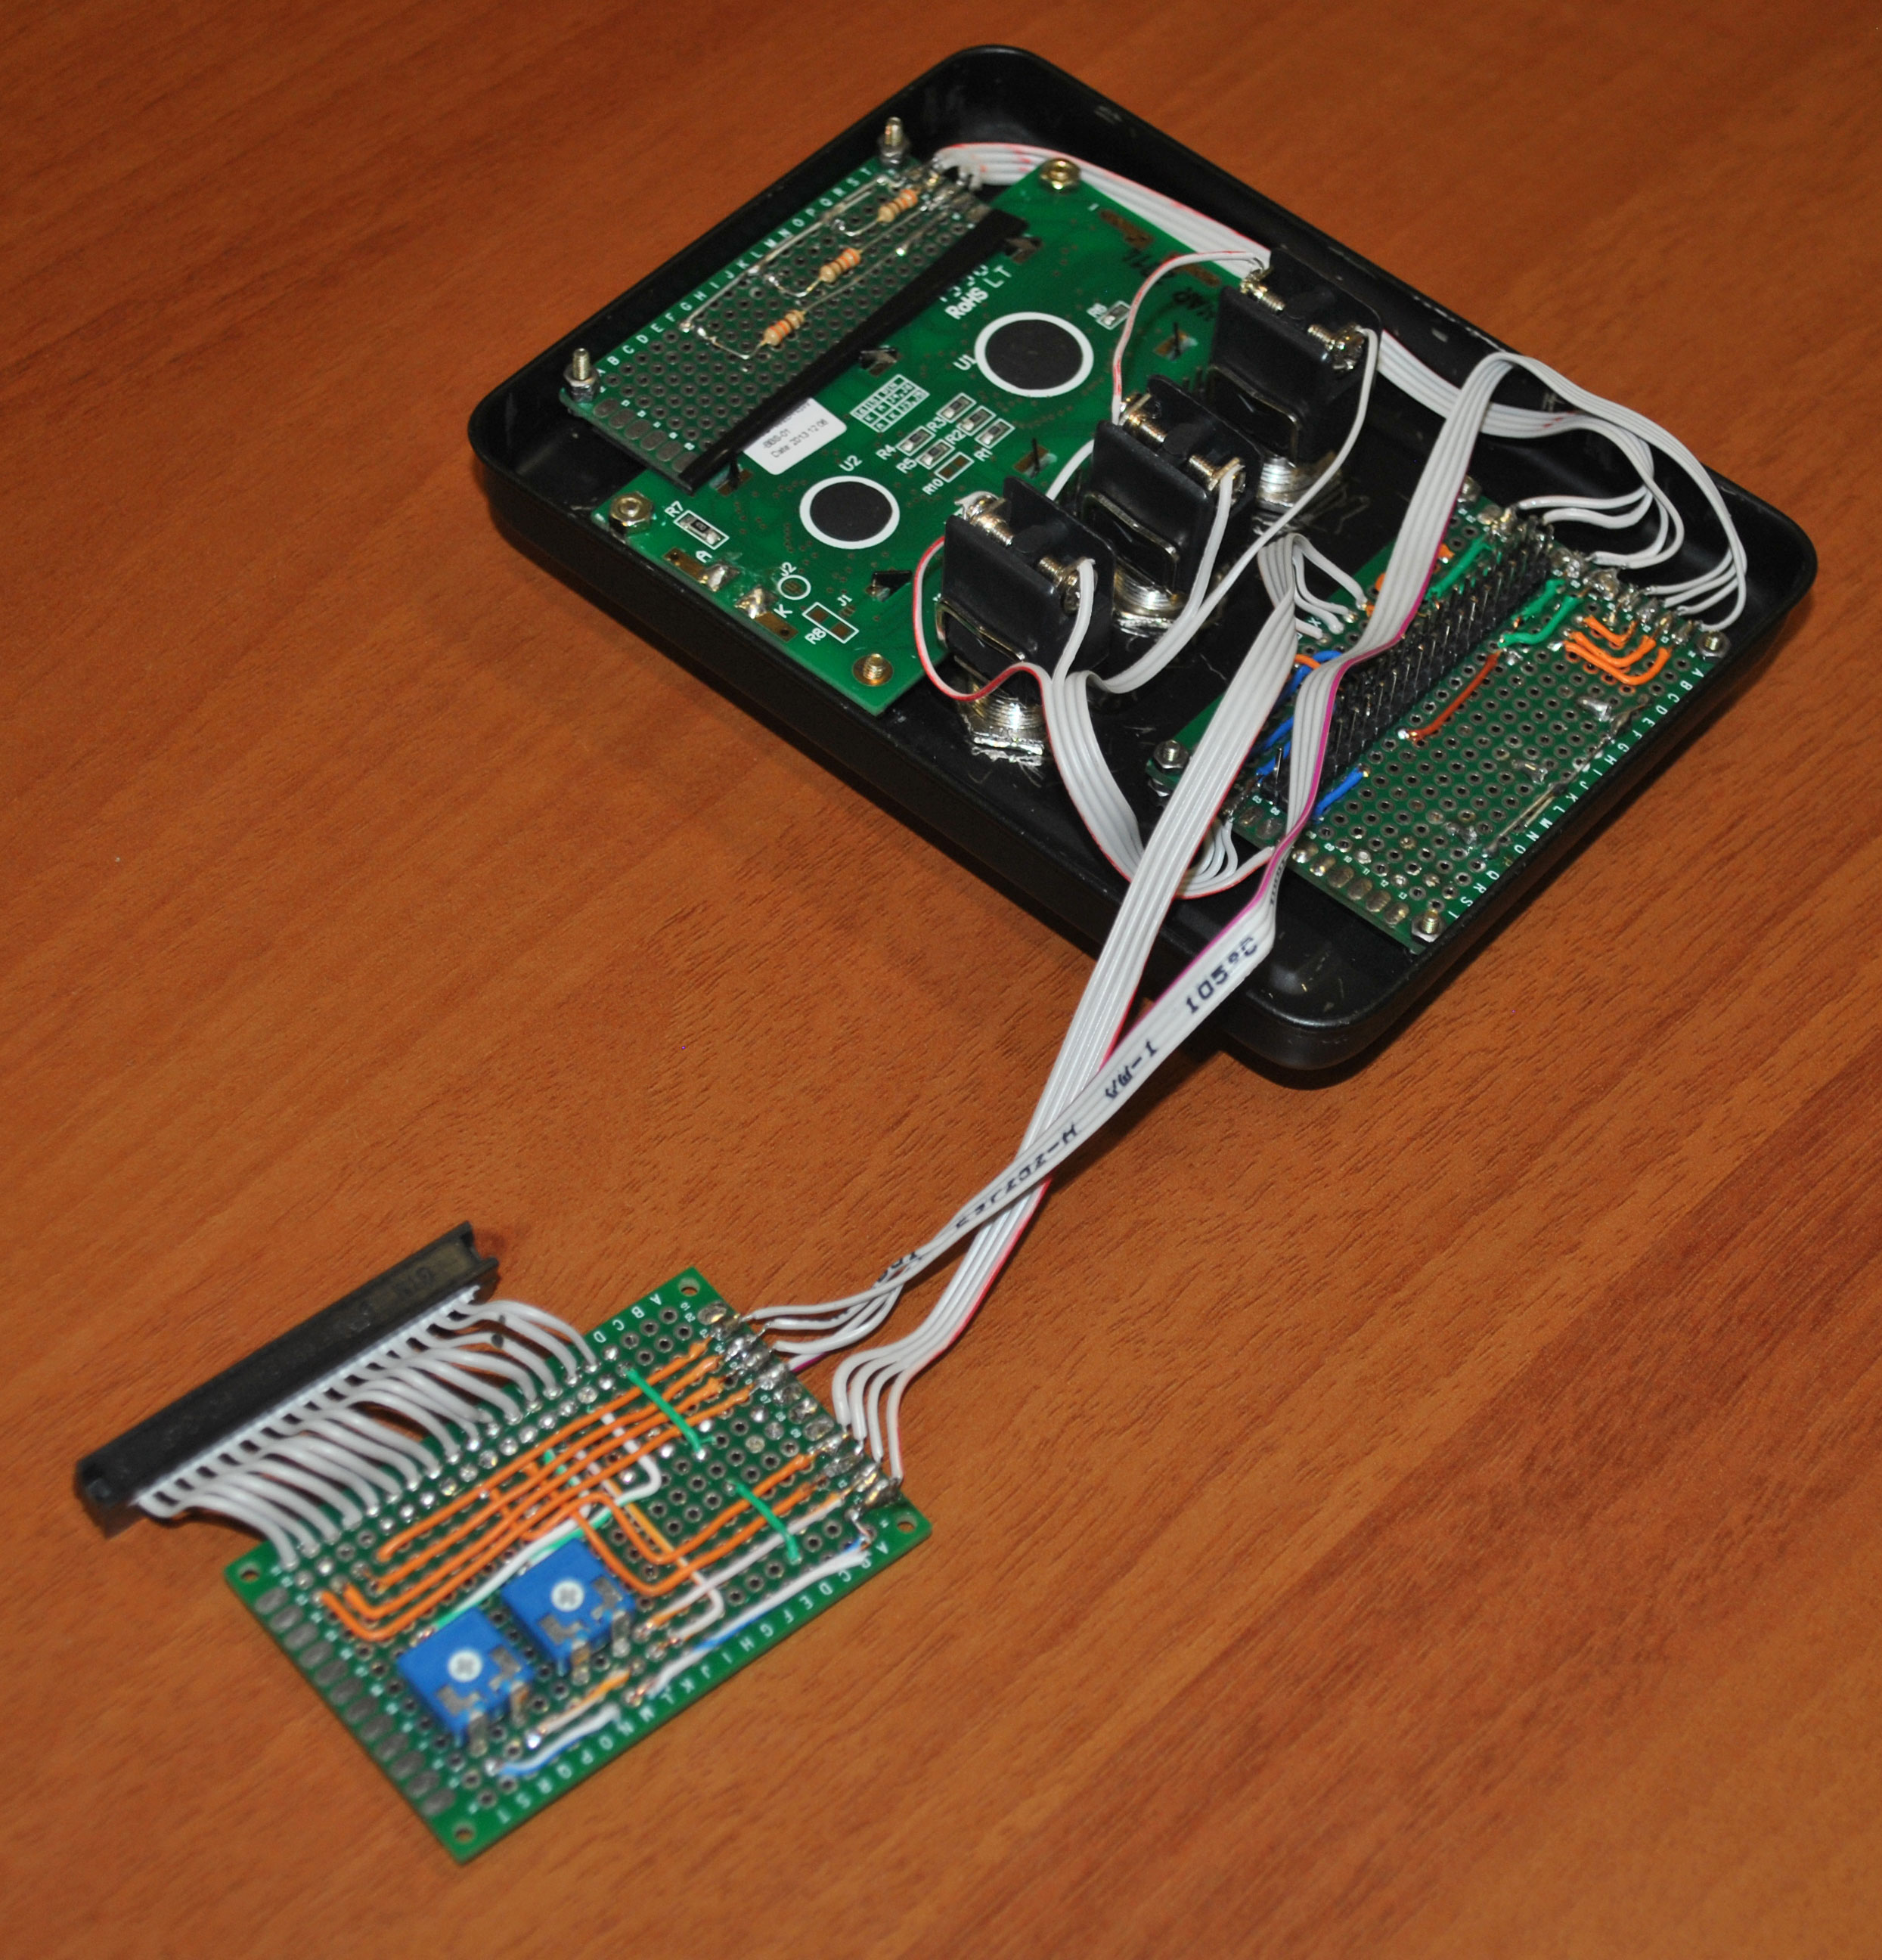
\includegraphics[width=1\textwidth]{img/interface-traz1.jpg}
		\legend{Fonte: elaborado pelo autor}
	\end{minipage}
	\hfill
	\begin{minipage}{0.45\textwidth}
		\centering
		\caption{\label{fig:interface-traz2}Parte interna da interface - completamente montada}
		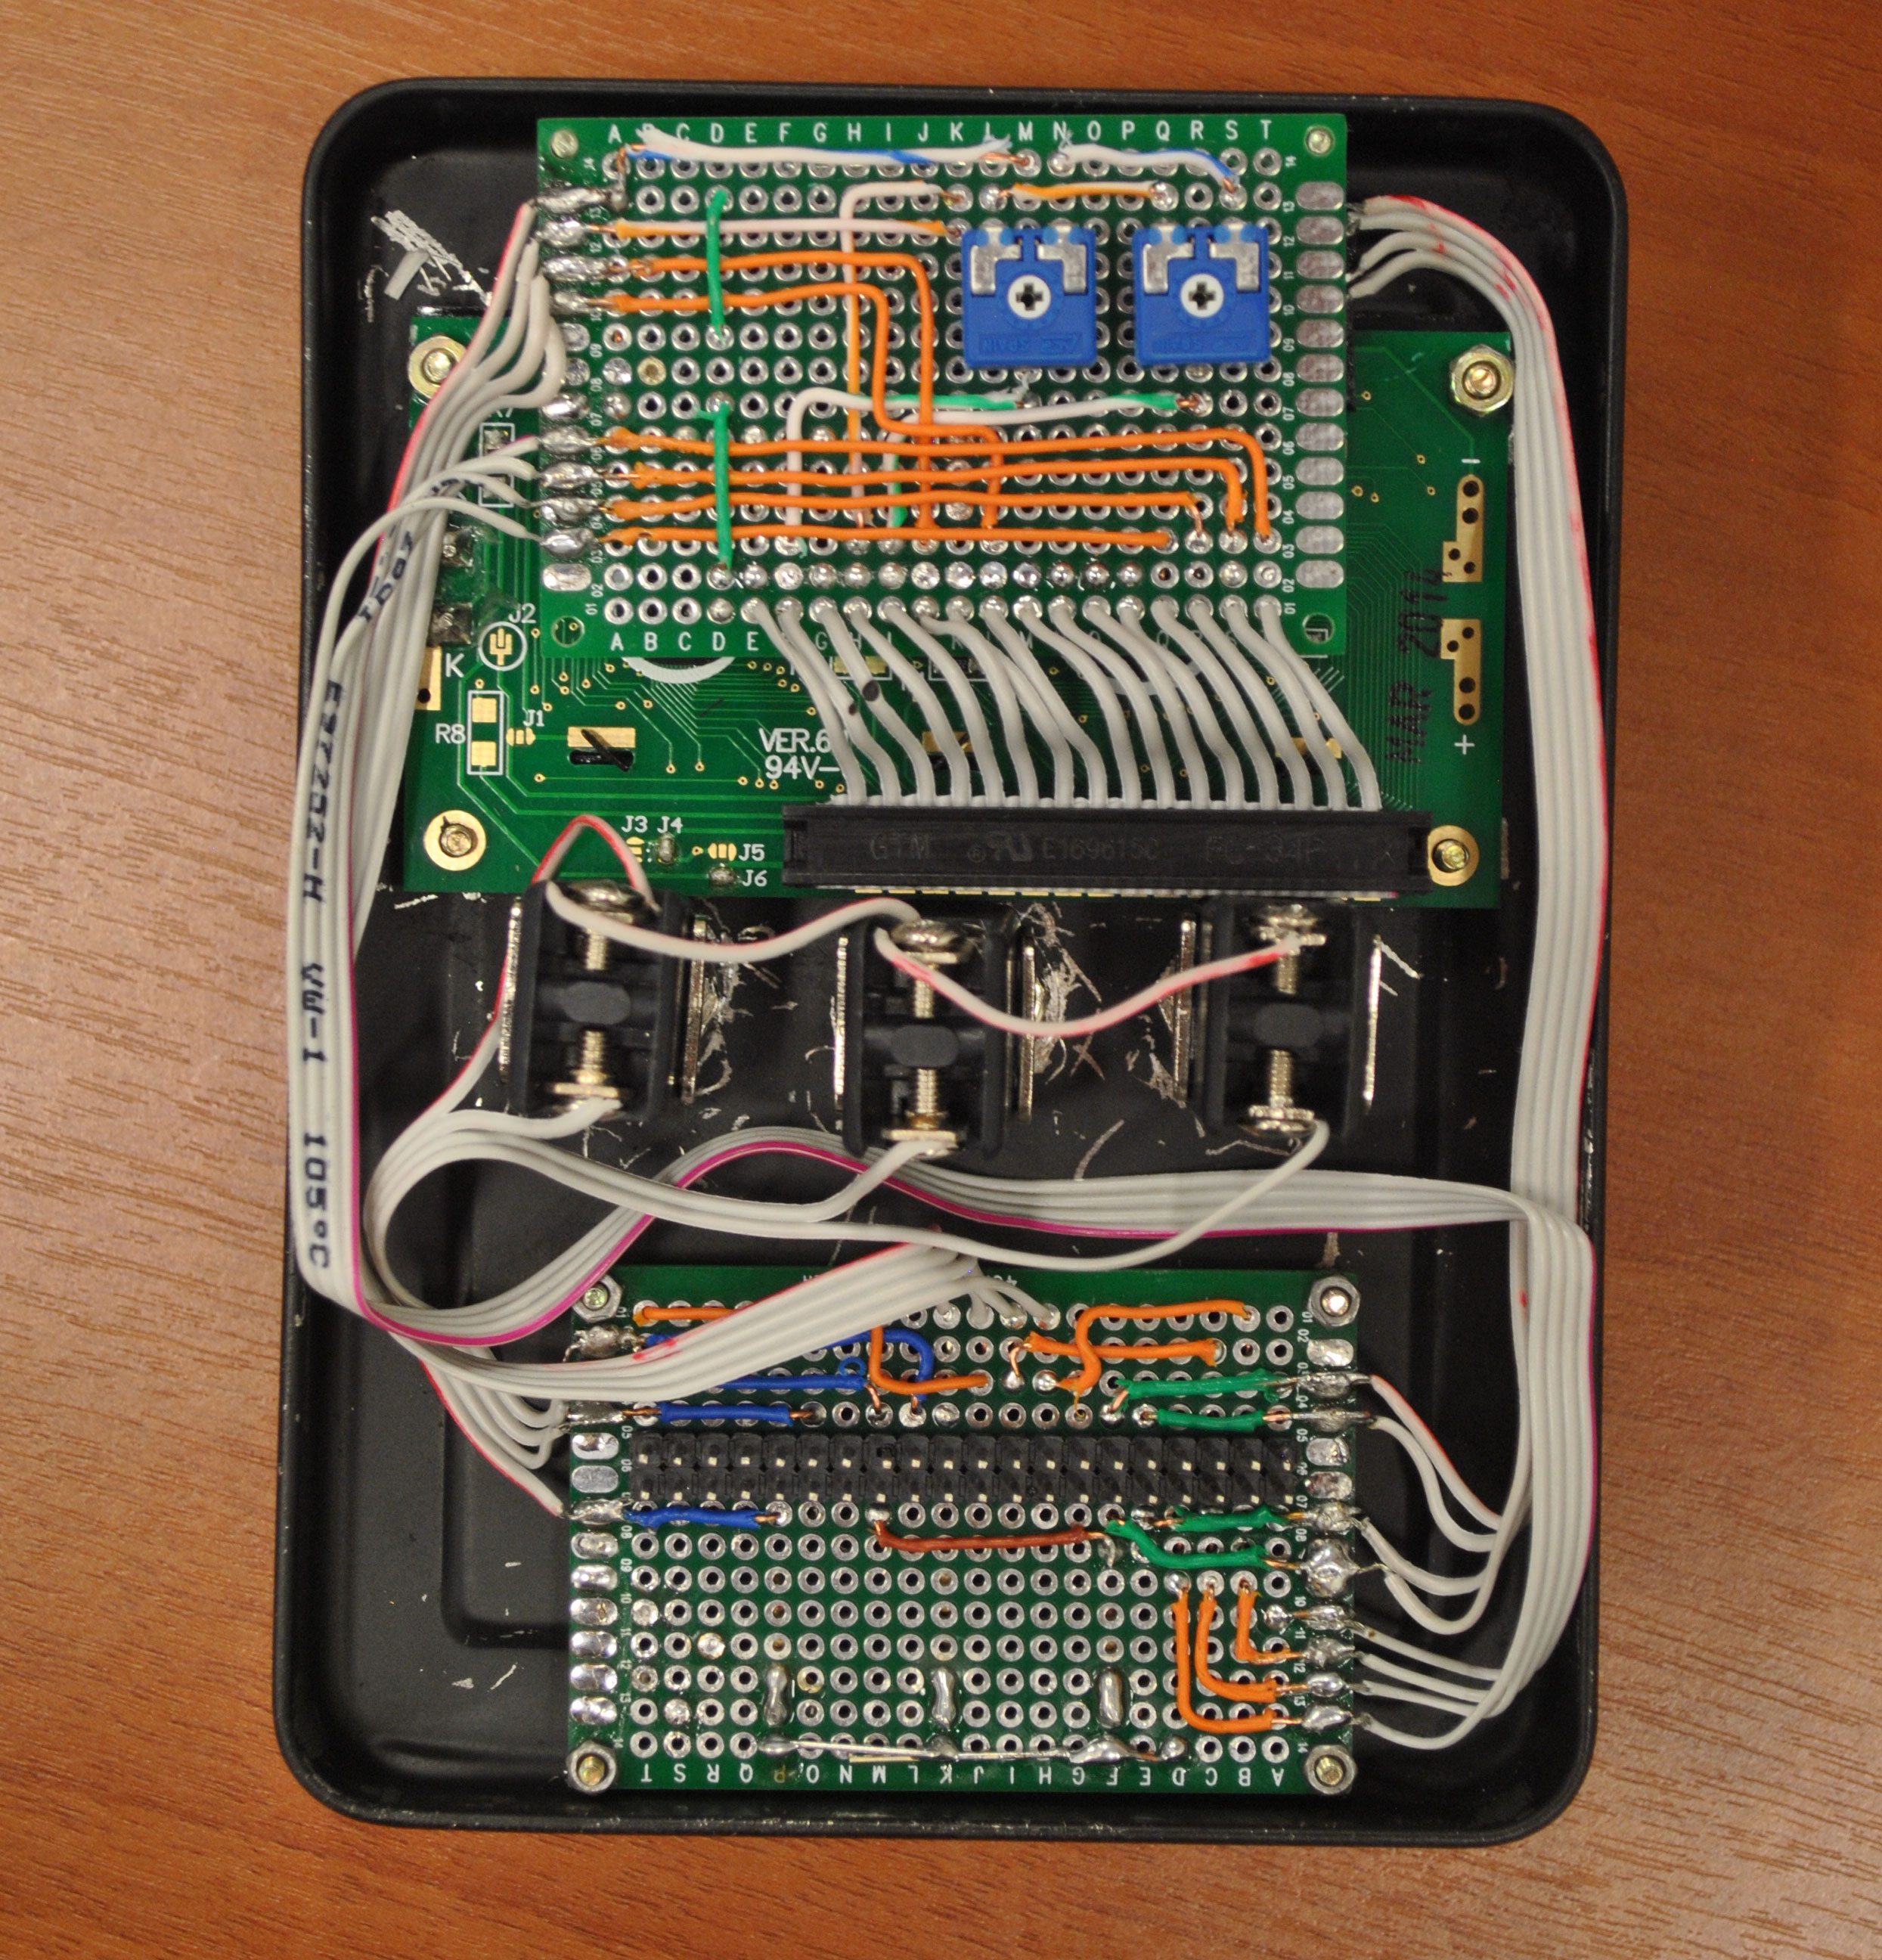
\includegraphics[width=1\textwidth]{img/interface-traz2.jpg}
		\legend{Fonte: elaborado pelo autor}
	\end{minipage}
\end{figure}

As placas internas da interface foram afixadas com cola quente, para que os cabos fossem reforçados e nenhuma conexão fosse quebrada. Tampa e base foram conectados com o cabo flat (\autoref{fig:tampa-base}) e o protótipo ficou pronto para desenvolvimento da aplicação.

\begin{figure}[htb]
	\centering
 	\begin{minipage}{0.45\textwidth}
		\centering
		\caption{\label{fig:tampa-base}Conexão da tampa com a base}
		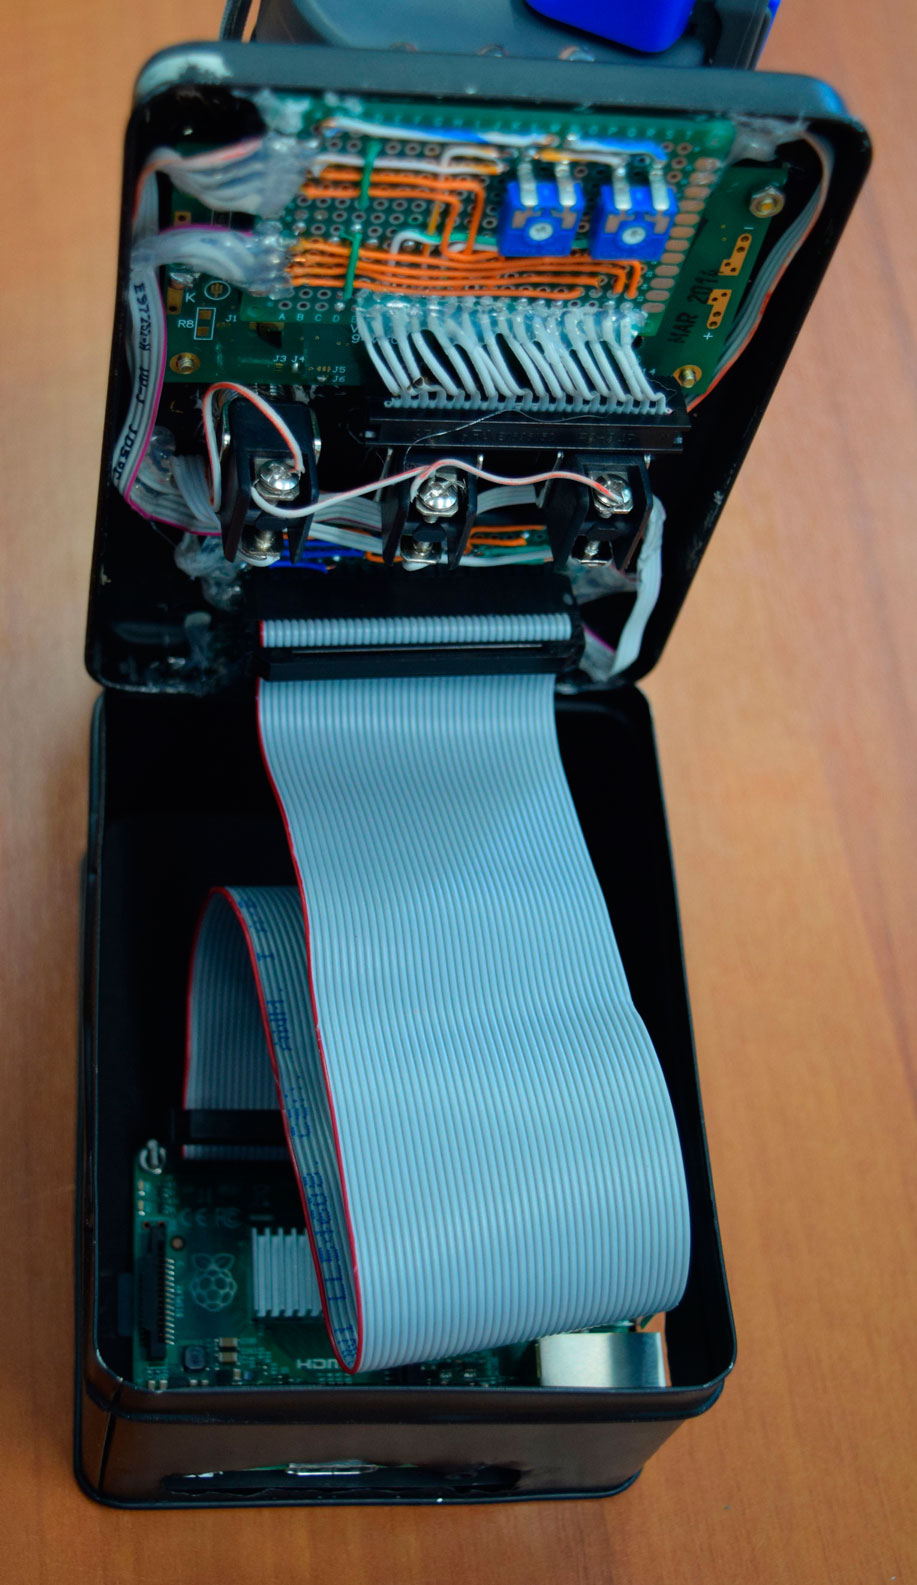
\includegraphics[width=0.84\textwidth]{img/tampa-base.jpg}
		\legend{Fonte: elaborado pelo autor}
	\end{minipage}
	\hfill
	\begin{minipage}{0.45\textwidth}
		\centering
		\caption{\label{fig:prot-final}Criação e montagem do protótipo finalizada}
		\includegraphics[width=1\textwidth]{img/prot-final-2.jpg}
		\legend{Fonte: elaborado pelo autor}
	\end{minipage}
\end{figure}

Após o hardware estar totalmente montado, as informações apresentadas nas telas foram elaboradas:

\begin{alineas}
	\item A primeira tela mostra informações sobre os beacons no alcance, ou caso não haja nenhum, apresenta o texto "\textit{Aguardando beacons}". As subtelas apresentam informações sobre quais beacons estão no alcance, sendo o nome atribuidos a eles ou então o texto "\textit{Desconhecido}"\ caso não esteja no banco de dados. A quantidade de subtelas depende da quantidade de beacons no alcance, por isso não se sabe ao certo a quantidade total;
	\item A segunda tela apresenta um histórico dos beacons encontrados durante a execução do programa, com um contador da quantidade de beacons no histórico, e as subtelas apresentam o nome do beacon encontrado em ordem numérica. Se um beacon for encontrado diversas vezes, será repetido nas subtelas. Conforme a primeira tela, a quantidade de subtelas depende da quantidade de beacons no histórico, por isso não se sabe ao certo a quantidade total;
	\item A terceira tela apresenta informações relevantes sobre o sistema, sendo elas:
	\begin{subalineas}
		\item Primeira subtela apresenta o \textit{load average}\footnote{Segundo \citeonline{load-average}, essa informação de três números apresenta a média de carga da CPU por um certo tempo. O primeiro número é a média no último minuto, o segundo número é a média nos últimos cinco minutos, e o terceiro número é a média nos últimos quinze minutos} do sistema Linux. É relevante para saber se o sistema está muito carregado ou trabalhando tranquilamente;
		\item Segunda subtela apresenta a temperatura do processador. É relevante para saber se o sistema está trabalhando a uma temperatura segura ou está sobreaquecendo;
		\item Terceira subtela apresenta o endereço de IP privado da rede. É de extrema importância para conexão remota, pois é esse endereço que é utilizado para conexão via \textit{SSH};
		\item Quarta subtela apresenta o endereço de IP público da rede. É relevante para saber se está conectado direto a internet (o IP privado será igual ao IP público) ou em uma subrede, como de uma residência ou do laboratório.
	\end{subalineas}
\end{alineas}

Após todos esses passos o protótipo estava bem definido para o desenvolvimento.


% ---
\subsection{Problemas Enfrentados}\label{sec:problemas-enfrentados}
% ---

Durante os estudos e testes dos LEDs na protoboard utilizou-se resistores de 330$\Omega$ para conexão correta. Quanto maior o valor da resistência, menor brilho o LED apresenta. Como os componentes estavam na protoboard, não percebeu-se que os LEDs utilizados eram de alto brilho.

Para soldagem final dos componentes, preferiu-se por manter os resistores de 330$\Omega$ por questões práticas. Porém os LEDs ficaram com muito brilho, incomodando qualquer pessoa que olhasse diretamente para o protótipo, conforme \autoref{fig:led-forte-1} e \autoref{fig:led-forte-2}.

\begin{figure}[htb]
	\centering
 	\begin{minipage}{0.45\textwidth}
		\centering
		\caption{\label{fig:led-forte-1}LED de alto brilho ao olhar diretamente}
		\includegraphics[width=1\textwidth]{img/led-forte-1.jpg}
		\legend{Fonte: elaborado pelo autor}
	\end{minipage}
	\hfill
	\begin{minipage}{0.45\textwidth}
		\centering
		\caption{\label{fig:led-forte-2}LEDs de alto brilho refletindo na mesa}
		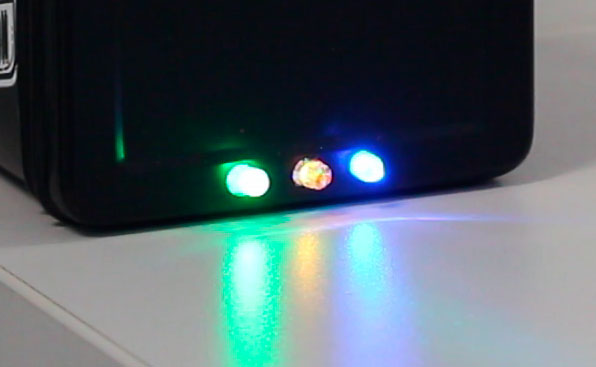
\includegraphics[width=1\textwidth]{img/led-forte-2.jpg}
		\legend{Fonte: elaborado pelo autor}
	\end{minipage}
\end{figure}

Como os componentes já estavam afixados com cola quente, substituir os resistores levaria muito tempo e possivelmente atrasaria o desenvolvimento do projeto, portanto optou-se por manter dessa maneira. Para um futuro protótipo, resistores maiores, ou LEDs com menos brilho podem ser utilizados.

% ----------------------------------------------------------
\section{Terceira Etapa - Desenvolvimento e Testes da Aplicação}\label{sec:terceira-etapa}
% ----------------------------------------------------------

A aplicação foi dividida em módulos por maior facilidade de desenvolvimento, testes e descoberta de erros. Um arquivo de configurações globais, nomeado \textit{globals-config.js}, foi utilizado para todas as definições de constantes de forma a facilitar futuras mudanças, caso necessário. 

% ---
\subsection{Primeiro Módulo - Biblioteca Auxiliar}\label{sec:primeiro-modulo}
% ---

O primeiro módulo desenvolvido foi a interface, que consiste da conexão com LEDs, botões e display LCD. Optou-se por criar uma biblioteca auxiliar para abstrair métodos repetitivos e também irrelevantes para os outros módulos. Como esse módulo é o meio de acesso do código principal aos componentes de hardware, foram adicionados trechos de teste para acender o LED e apagar o LED pela linha de comando, de forma que os testes de funcionalidade pudessem ser realizados.

Durante a fase de testes do primeiro módulo, um fato interessante ocorreu. Ao clicar uma única vez em um botão, em algumas vezes o código executava dois, três ou até mais cliques de botão. Pesquisando mais a fundo sobre esse erro, uma informação nova surgiu. 

Botões mecânicos não criam ou perdem o contato corretamente, conforme caso ideal e perfeito representado no Gráfico~\ref{fig:debounce-graph-1}. Em vez disso, podem oscilar rapidamente no momento do clique ou ao soltar o botão, conforme Gráfico~\ref{fig:debounce-graph-2}. \cite{debounce-graph}. Esse efeito é conhecido como \textit{bounce}, ou ruído.

\begin{figure}[htb]
	\centering
 	\begin{minipage}{0.45\textwidth}
		\centering
		\caption{\label{fig:debounce-graph-1}Gráfico ideal de um clique de botão}
		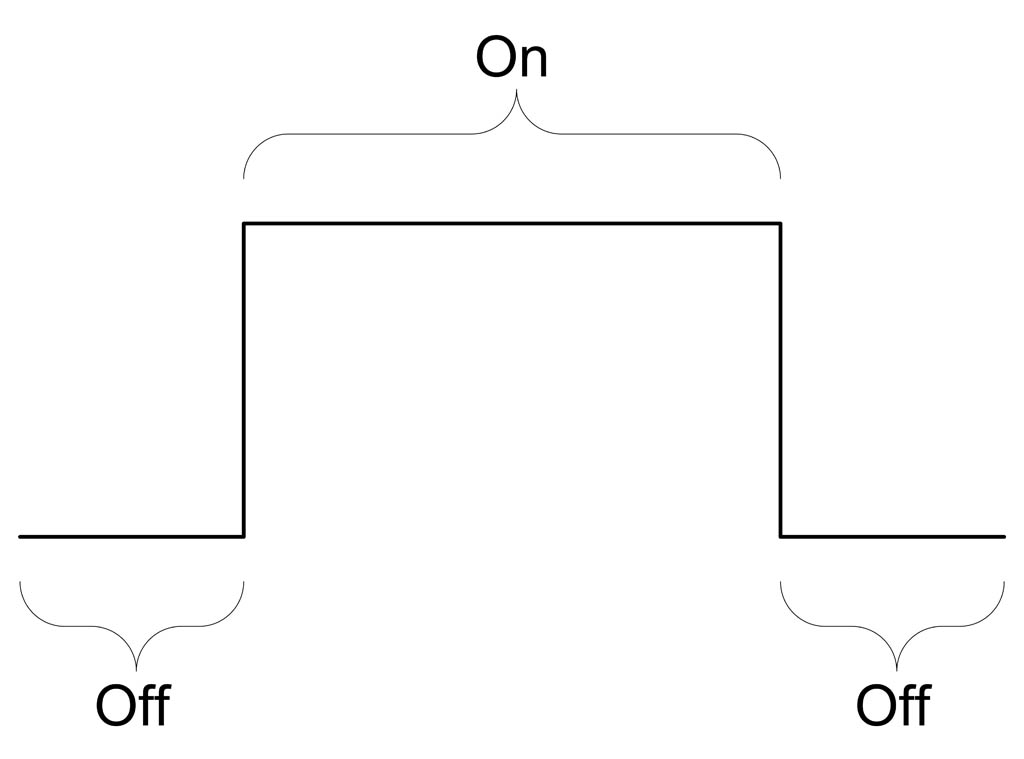
\includegraphics[width=0.8\textwidth]{img/debounce-graph-1.jpg}
		\legend{Fonte: \cite{debounce-graph}}
	\end{minipage}
	\hfill
	\begin{minipage}{0.45\textwidth}
		\centering
		\caption{\label{fig:debounce-graph-2}Gráfico real de um clique de botão}
		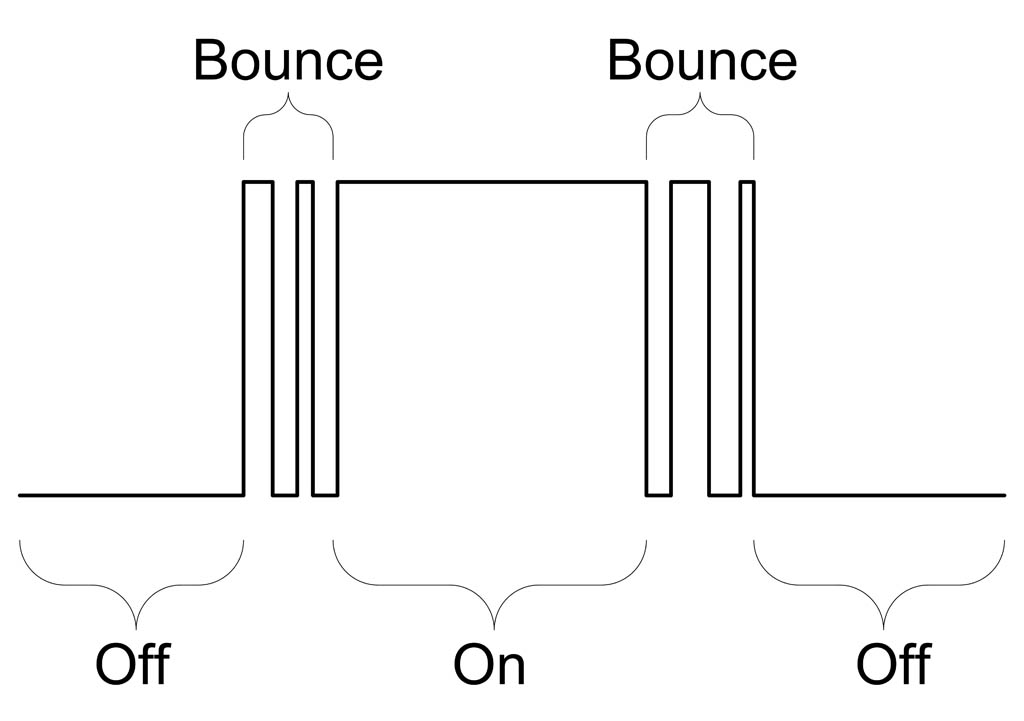
\includegraphics[width=0.8\textwidth]{img/debounce-graph-2.jpg}
		\legend{Fonte: \cite{debounce-graph}}
	\end{minipage}
\end{figure}

A solução para resolver esse problema (denominada \textit{debounce}) foi de bloquear todos os cliques após o primeiro clique via programação por determinado tempo (em milissegundos), de forma que não interferisse diretamente nos cliques reais do usuário. Esse tempo foi determinado por testes repetitivos e por diferentes usuários em 200ms. Esse valor foi considerado ideal por evitar o ruído e não interferir em cliques seguidos do usuário. Valores maiores, como 300ms afetaram o clique do usuário, e valores inferiores como 100ms não evitaram totalmente o ruído.

% ---
\subsection{Segundo Módulo - Páginas e Navegação}\label{sec:segundo-modulo}
% ---

Páginas e Navegação entre telas

% ---
\subsection{Terceiro Módulo - Identificação dos Beacons}\label{sec:terceiro-modulo}
% ---

Identificação dos Beacons e apresentação nas telas corretas

% ---
\subsection{Quarto Módulo - Busca no Banco de Dados}\label{sec:quarto-modulo}
% ---

Procurar beacon no banco de dados local

% ---
\subsection{Quinto Módulo - Salvar no Banco de Dados}\label{sec:quinto-modulo}
% ---

Salvar beacons encontrados no banco de dados local

% ---
\subsection{Protótipo Finalizado}\label{sec:prototipo-final}
% ---

Mostrar logo e falar sobre protótipo final

\begin{figure}[htb]
	\caption{\label{fig:prod-final}Protótipo finalizado e totalmente funcional}
	\begin{center}
		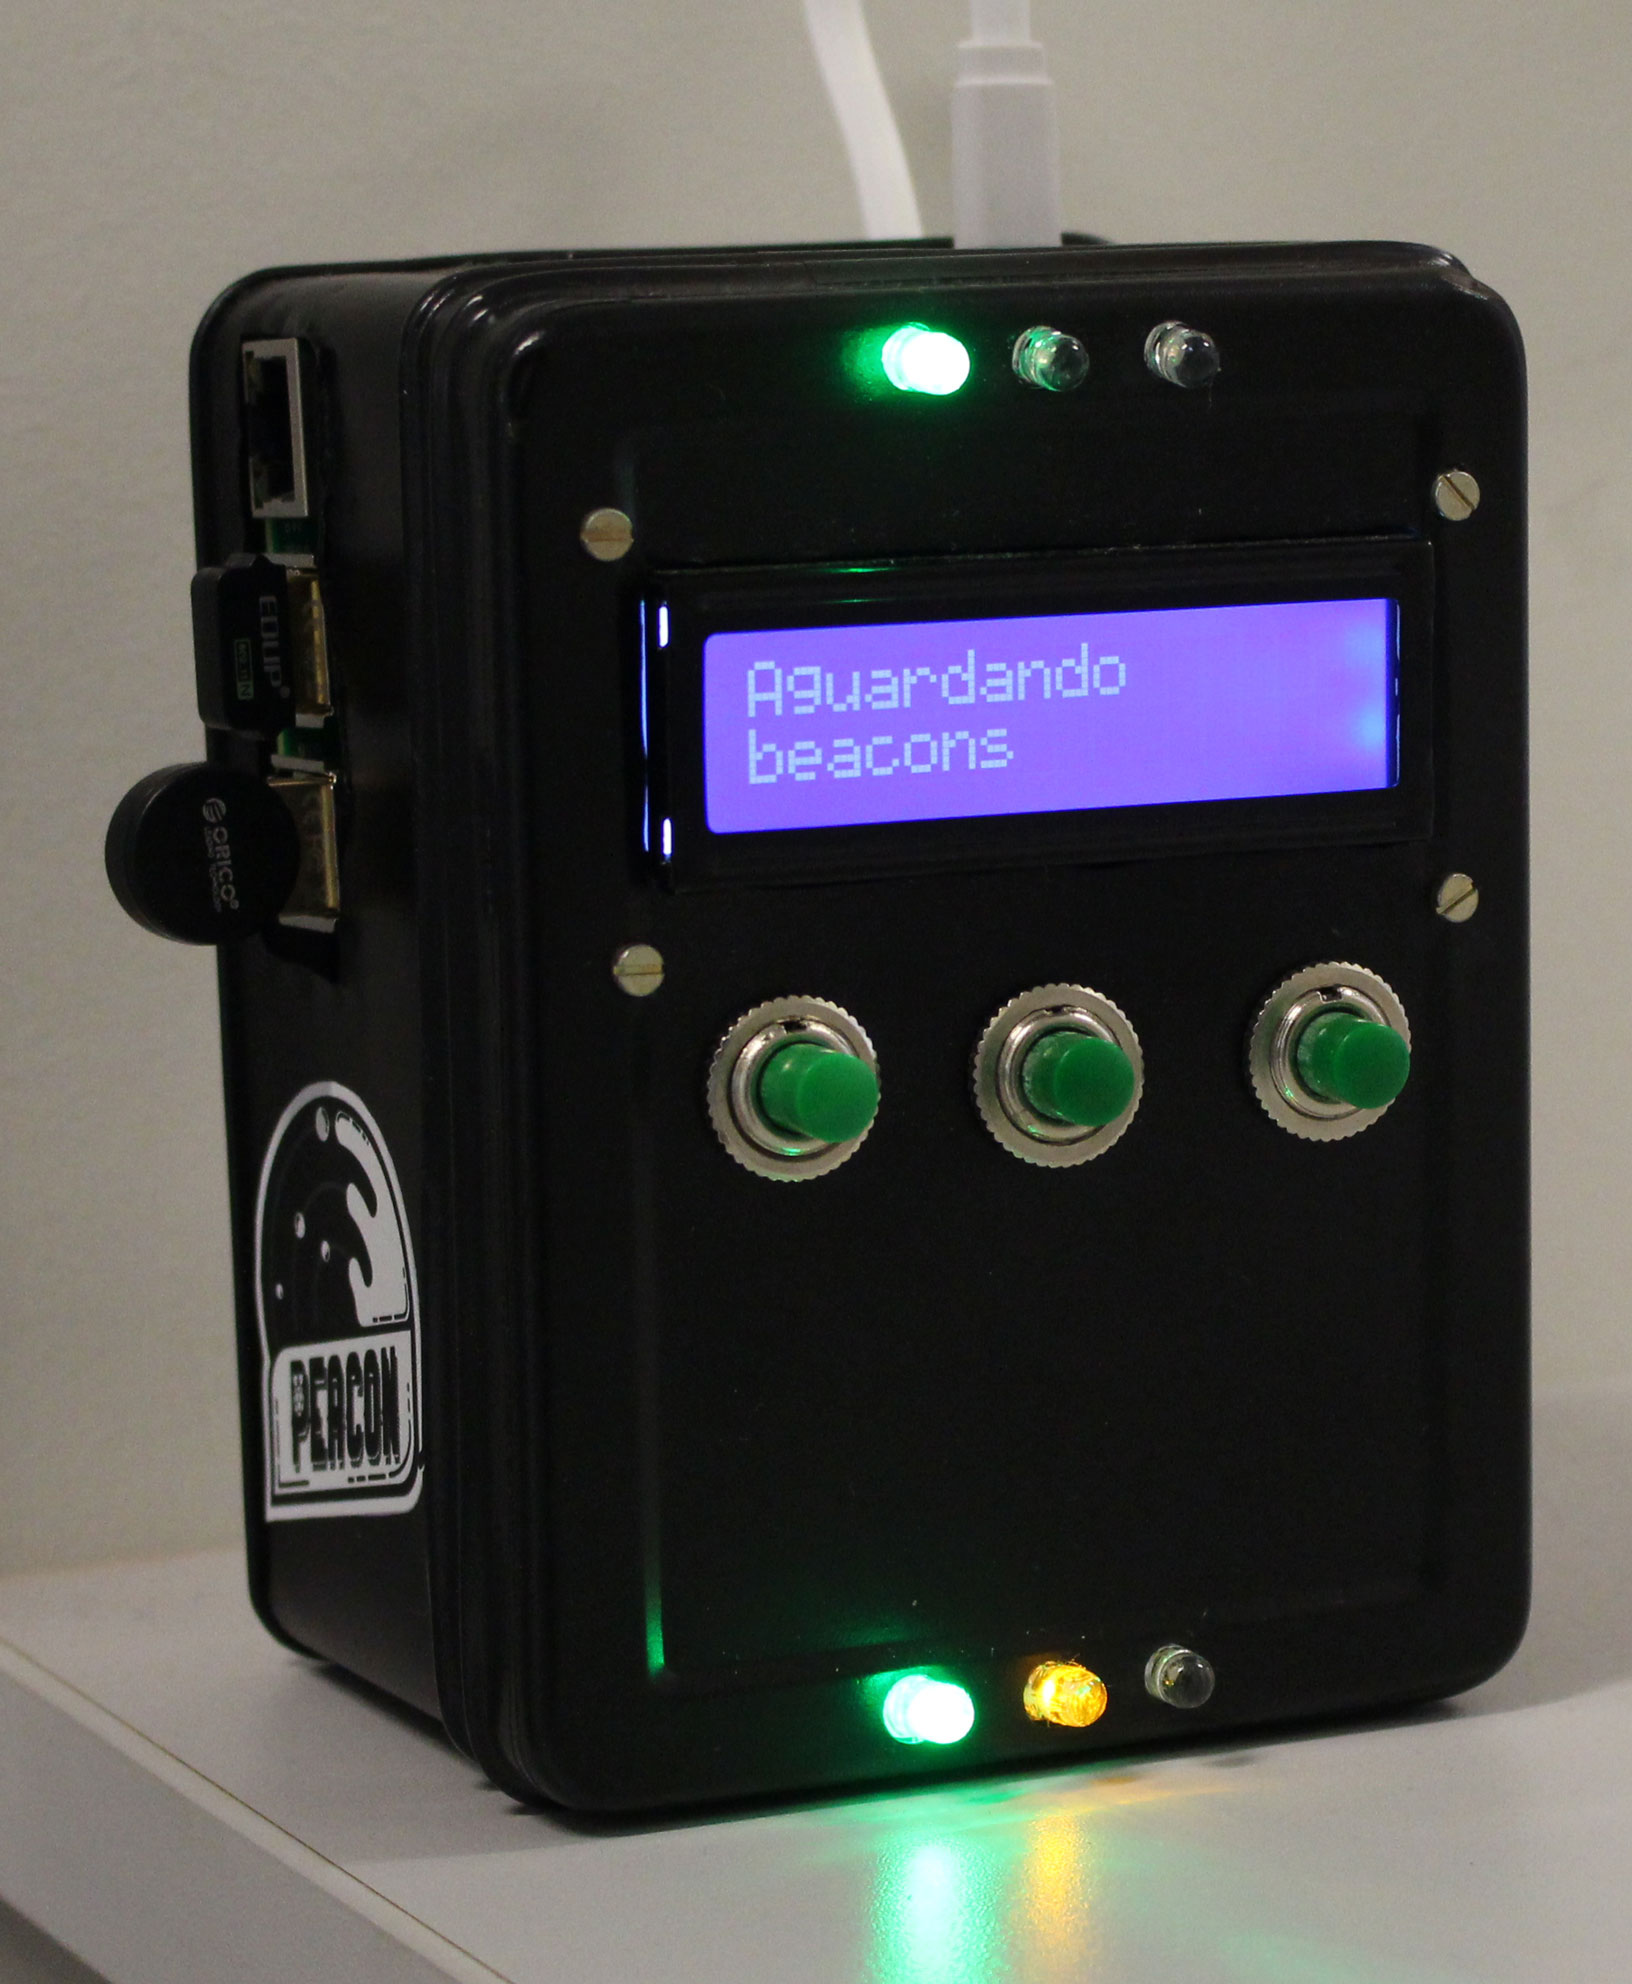
\includegraphics[width=0.8\textwidth]{img/prod-final.jpg}
	\end{center}
	\legend{Fonte: elaborado pelo autor}
\end{figure}

% ----------------------------------------------------------


% ----------------------------------------------------------
% Conclusão
% ----------------------------------------------------------
\chapter{Conclusão}
% ----------------------------------------------------------

FALTA ACERTAR!!!! Esse projeto tem como objetivo o aprofundamento na área de Internet das Coisas, pelo estudo das tecnologias de \textit{Bluetooth Low Energy}, \textit{Raspberry Pi} e \textit{beacons}. O resultado final será um protótipo de rastreador de \textit{beacons} utilizando o \textit{Raspberry Pi}, ainda em desenvolvimento.

A fundamentação teórica realizada por meio de pesquisa bibliográfica no início do projeto foi essencial para entender como os protocolos \textit{beacons} foram propostas e implementadas, como é o comportamento do \textit{Raspberry Pi}, entre outros. Em conjunto, o estudo das tecnologias foi de extrema importância para entender o funcionamento e utilização do \textit{RPi} e \textit{beacon}.

Certas atividades de extrema importancia ainda serão realizadas, mas o projeto ainda tem muitos frutos para render, caminhando em uma boa direção. A área de Internet das Coisas é uma área extremamente promissora, com áreas de pesquisa e implementação bem vastas. 

% ----------------------------------------------------------

% ----------------------------------------------------------------------------------------------------------------------------------



% ----------------------------------------------------------
% ELEMENTOS PÓS-TEXTUAIS
% ----------------------------------------------------------

% ----------------------------------------------------------
% Referências bibliográficas
% ----------------------------------------------------------
\bibliography{referencias}
% ----------------------------------------------------------

% ----------------------------------------------------------
% Apêndices
% ----------------------------------------------------------

% ---
% Inicia os apêndices
% ---
\begin{apendicesenv}

% Apendice - LaTeX

% ----------------------------------------------------------
\chapter{LaTeX}\label{ap:latex}
% ----------------------------------------------------------

Para o desenvolvimento dessa monografia utilizou-se uma ferramenta denominada TeX, um processador de texto baseado em comandos e macros. Normalmente é grafado usando a macro \texttt{\detokenize{\TeX}}, resultando em \TeX. 

Não é comum o uso do \TeX\ por si só. Utiliza-se uma outra ferramenta denominada LaTeX (grafada \LaTeX), uma série de macros definidas para auxiliar o desenvolvimento.

Essa abordagem é muito utilizada no meio acadêmico e científico, pois o ponto mais importante dessa ferramenta é o conteúdo. O design final ficará sempre para o compilador gerar. Isso evita erros de formatação, como por exemplo devido a diferenças entre versões de programas.

Congressos e revistas científicas já disponibilizam arquivos no formato \texttt{.sty}\footnote{Modelo de estilos \TeX.} para que os pesquisadores enviem os artigos preenchidos em \texttt{.pdf} formatado conforme modelo próprio. Dessa forma todos os artigos seguirão o mesmo formato, auxiliando também os pesquisadores a escreverem os documentos rapidamente.

Por ser um documento de texto no formato \texttt{.tex}, qualquer editor comum como o Bloco de Notas do Windows pode ser utilizado. Dessa forma a compilação é feita por meio da linha de comando, com algumas opções de compiladores. As mais utilizadas são \texttt{pdflatex} e \texttt{xelatex}.

O meio mais utilizado para escrita de documentos \LaTeX\ de forma a facilitar a compilação são programas próprios. Existem diversas opções, mas as mais utilizadas são MiKTeX\footnote{\url{http://miktex.org/}} para Windows e MacTeX\footnote{\url{http://tug.org/mactex}} para Mac OSX. O programa utilizado para esse documento foi o TeXworks, um editor de texto para \TeX\ multiplataforma e de código aberto, conforme imagem \ref{fig:texworks}.

\begin{figure}[htb]
	\caption{\label{fig:texworks}TeXworks, programa utilizado para escrever o código \TeX}
	\begin{center}
		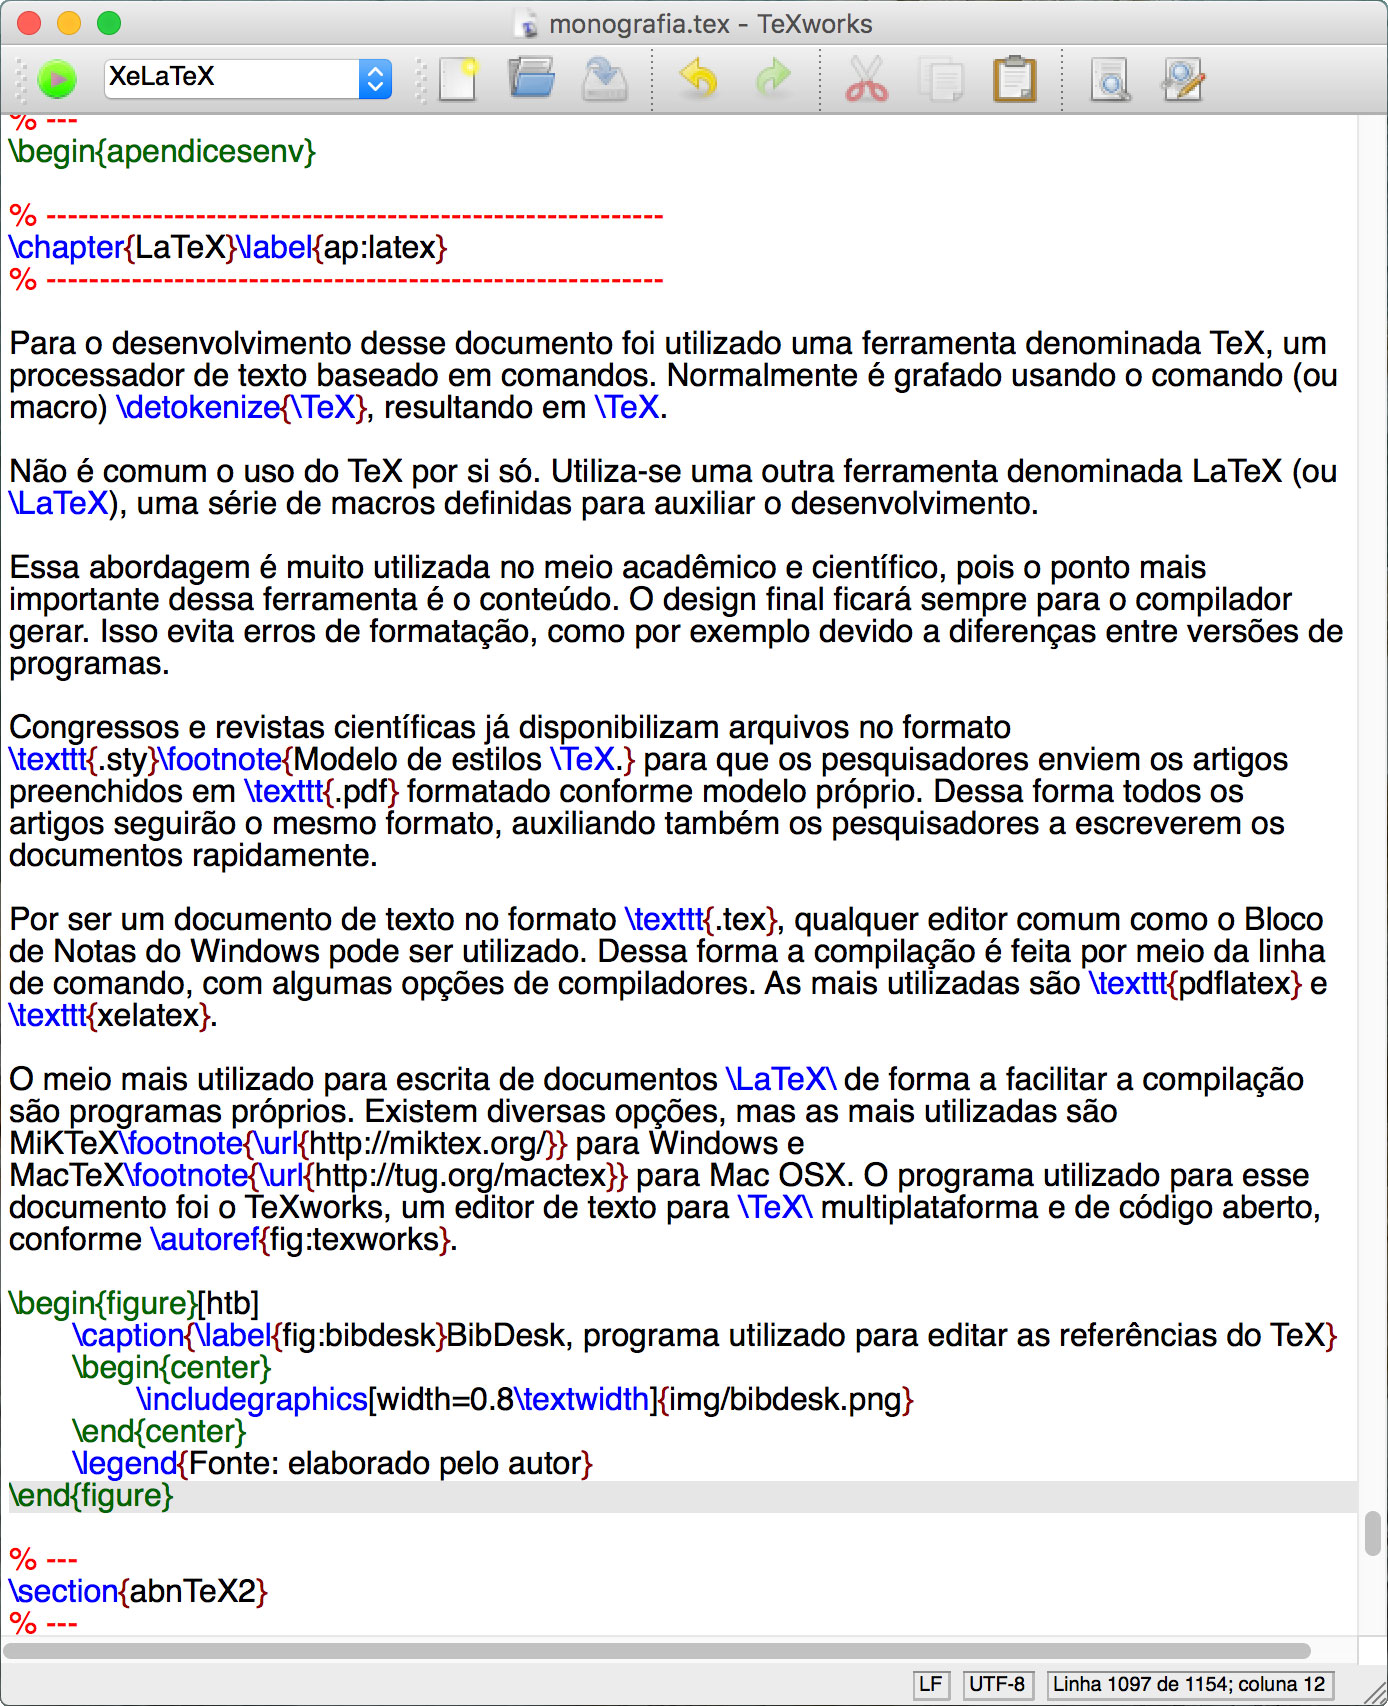
\includegraphics[width=0.65\textwidth]{img/texworks.jpg}
	\end{center}
	\legend{Fonte: elaborado pelo autor}
\end{figure}

% ---
\section{abnTeX2}
% ---

Devido a esse Trabalho de Conclusão de Curso seguir as normas ABNT\footnote{Associação Brasileira de Normas Técnicas.} para escrita e formatação de documentos científicos, utilizou-se a biblioteca de macros abnTeX2 (\abnTeX)\footnote{\url{https://github.com/abntex/abntex2}} para formatação do documento conforme as normas vigentes. Essa biblioteca é livre, com código fonte aberto e disponível para qualquer um auxiliar.

Uma ferramenta muito útil disponível com o \abnTeX\ é a criação das Referências Bibliográficas no formato ABNT de forma automática. Para tal, é criado um arquivo \texttt{.bib} com todas as informações de citações e referências utilizadas no texto.

As chaves de citação são os valores que serão utilizados nas macros do \abnTeX\ para que as referências sejam corretamente configuradas. Por exemplo, se desejamos referenciar um artigo de \citeonline{windows10-iot}, adicionamos todas as informações como nome dos autores, organização, data, edição, entre outros, e adicionamos a chave \texttt{windows10-iot}. 

Utilizando a macro \texttt{\detokenize{\cite{windows10-iot}}}, no local ficará o texto \cite{windows10-iot}, e nas referências será adicionado conforme modelo ABNT: \texttt{MICROSOFT. A Internet das suas coisas. https://dev.windows.com/pt-br/iot, 2015.} Para citações \textit{inline}, ou na mesma linha, o comando \texttt{\detokenize{\citeonline{windows10-iot}}} é utilizado, gerando o texto \citeonline{windows10-iot}.

O arquivo \texttt{.bib} pode ser criado manualmente ou por meio de programas. Para esse artigo foi utilizado o programa BibDesk\footnote{\url{http://bibdesk.sourceforge.net/}} para Mac OSX, conforme \autoref{fig:bibdesk}. Esse programa já cria o arquivo no formato correto com as chaves de citação configuradas.

\begin{figure}[htb]
	\caption{\label{fig:bibdesk}BibDesk, programa utilizado para editar as referências do TeX}
	\begin{center}
		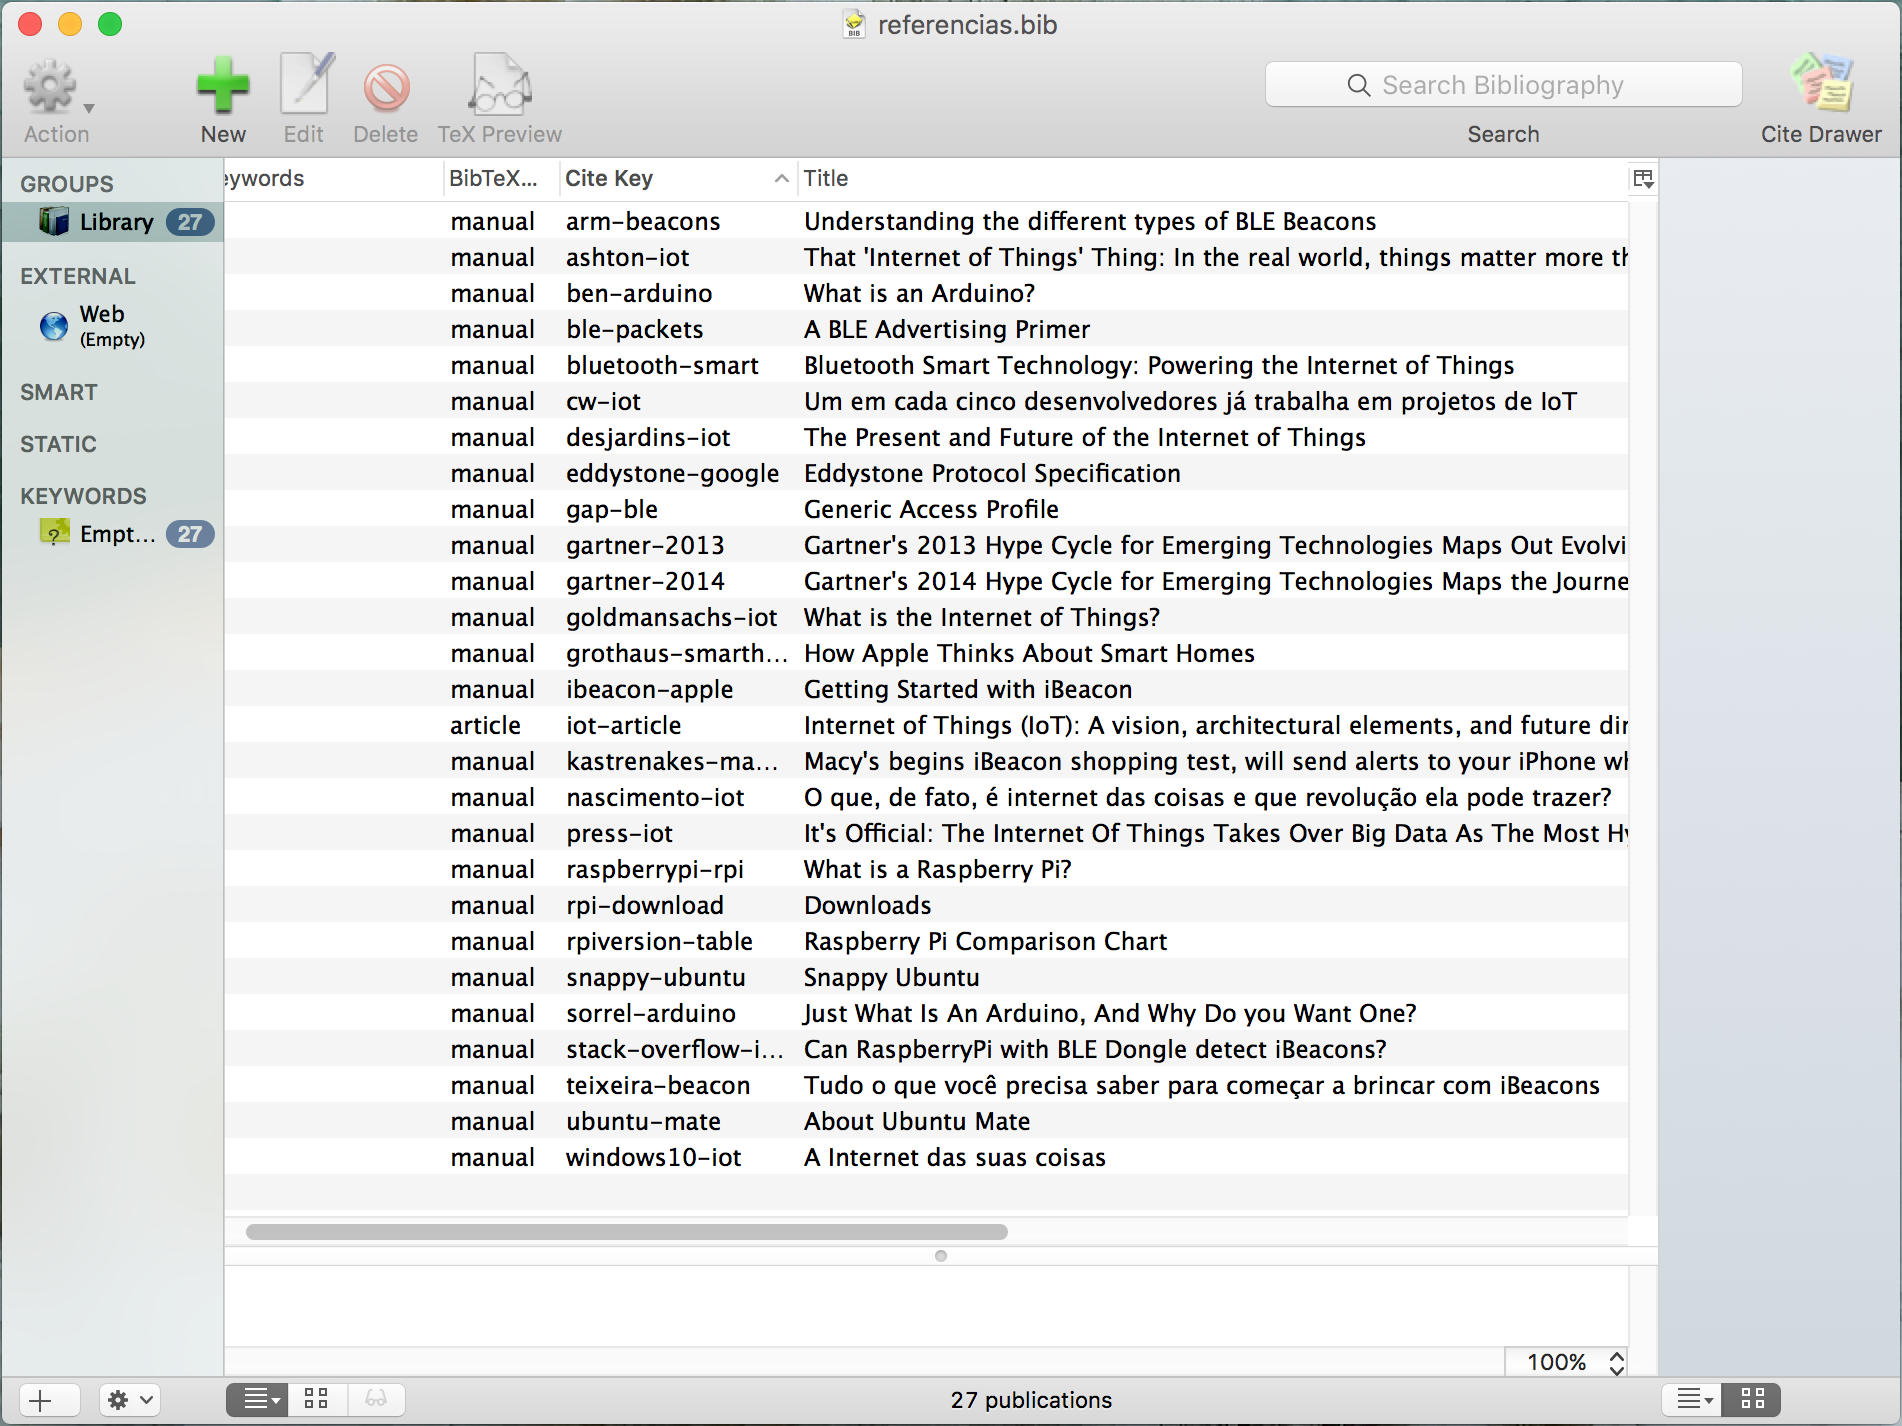
\includegraphics[width=0.8\textwidth]{img/bibdesk.png}
	\end{center}
	\legend{Fonte: elaborado pelo autor}
\end{figure}

Além de formatar o documento, \abnTeX\ também disponibiliza macros para criação de conteúdo citados na ABNT. Por exemplo, tabelas que seguem o formato do IBGE\footnote{Instituto Brasileiro de Geografia e Estatística} podem ser facilmente criadas com macros disponíveis, como exemplo da \autoref{table:ble-physical2}.

\begin{table}[htb]
     \IBGEtab{
          \caption{Exemplo de tabela gerada com o \LaTeX}
          \label{table:ble-physical2}
     }{
          \begin{tabular}{ccc}
               \toprule
                    & BLE & Classic \\
               \midrule \midrule
                    Modulação & GFSK 0.45 a 0.55 & GFSK 0.28 a 0.35 \\
               \midrule
                    Velocidade de Transferência & 1 Mbit/s & 1 Mbit/s \\
               \midrule 
                    Canais & 40 & 79 \\
               \midrule 
                    Espaçamento & 2 MHz & 1 MHz \\
               \bottomrule
          \end{tabular}
     }{
          \fonte{\cite{ble-packets}}
     }
\end{table}

O código para geração da \autoref{table:ble-physical2}, conforme a documentação da \abnTeX\, é:
\\ % para pular mais uma linha
\begin{verbatim}
\begin{table}[htb]
     \IBGEtab{
          \caption{\textit{BLE Physical Layer}}
          \label{table:ble-physical}
     }{
          \begin{tabular}{ccc}
               \toprule
                    & BLE & Classic \\
               \midrule \midrule
                    Modulação & GFSK 0.45 a 0.55 & GFSK 0.28 a 0.35 \\
               \midrule
                    Velocidade de Transferência & 1 Mbit/s & 1 Mbit/s \\
               \midrule 
                    Canais & 40 & 79 \\
               \midrule 
                    Espaçamento & 2 MHz & 1 MHz \\
               \bottomrule
          \end{tabular}
     }{
          \fonte{\cite{ble-packets}}
     }
\end{table}
\end{verbatim}

Diversas razões podem ser elencadas a favor do uso do \LaTeX\ e \abnTeX\ nessa monografia, entre elas:

\begin{alineas}
	\item Facilidade de criação do conteúdo: não é necessário criar o modelo do documento conforme as normas da ABNT, pois o \abnTeX\ já criará o documento final formatado;
	\item Evitar erros de formatação ao alterar o conteúdo do arquivo: muito comum quando utilizado o Microsoft Word, ao alterar o conteúdo de uma seção, as partes subsequentes facilmente perdem a formatação, sendo necessário uma revisão minunciosa para que esses erros sejam evitados;
	\item Continuação dos outros relatórios: como o autor gostaria de aprender essa tecnologia, utilizou para desenvolver a proposta desse trabalho. Portanto, para facilitar, continuou os outros relatórios utilizando a mesma ferramenta;
\end{alineas}

O código dessa monografia, assim como a versão final em \texttt{.pdf} pode ser acessado pelo repositório no GitHub\footnote{\url{https://github.com/gabrielboliveira/Monografia-Peacon}}. Está disponível para livre consulta, tanto de professores quanto de alunos interessados em saber mais sobre o \LaTeX.

\end{apendicesenv}
% ---

% ----------------------------------------------------------


\end{document}